% ============================================================
% main.tex - master documentation file
%
% Project : Learning Management System (Edvanta) - repository FSJP_LMS
% Purpose : Evidence-based product and technical documentation suite
% Output  : PDF (pdflatex), convertible to DOCX via Pandoc (see documents/README.md)
%
% Build:
%   pdflatex main.tex
%   pdflatex main.tex      (second pass resolves references)
%   (or: latexmk -pdf main.tex)
% ============================================================
\documentclass[11pt,a4paper]{article}

% ============================================================
% preamble.tex - shared style and package configuration
% Target engines: pdflatex (primary), xelatex (compatible)
% Designed for clean conversion workflows (standard constructs only)
% ============================================================

% --- Encoding and fonts ---
\usepackage[utf8]{inputenc}
\usepackage[T1]{fontenc}
\usepackage{lmodern}
\usepackage[english]{babel}
\usepackage{microtype}

% --- Page layout ---
\usepackage[a4paper,margin=2.4cm,top=3.0cm,bottom=2.6cm,headheight=14pt]{geometry}
\usepackage{setspace}
\setstretch{1.08}

% --- Graphics and colour ---
\usepackage{graphicx}
\usepackage{xcolor}
\definecolor{linkblue}{HTML}{1A4B8C}
\definecolor{codedark}{HTML}{1E1E1E}
\definecolor{codebg}{HTML}{F4F4F5}
\definecolor{rulegrey}{HTML}{BFBFBF}
\definecolor{statusgreen}{HTML}{1A7F4B}
\definecolor{statusred}{HTML}{C02626}
\definecolor{statusamber}{HTML}{A34E12}

% --- Tables ---
\usepackage{array}
\usepackage{booktabs}
\usepackage{tabularx}
\usepackage{longtable}
\usepackage{multirow}
\newcolumntype{L}[1]{>{\raggedright\arraybackslash}p{#1}}
\newcolumntype{C}[1]{>{\centering\arraybackslash}p{#1}}
\newcolumntype{R}[1]{>{\raggedleft\arraybackslash}p{#1}}

% --- Floats, captions, cross references ---
\usepackage{float}
\usepackage{caption}
\captionsetup{font=small,labelfont=bf,skip=6pt}
\usepackage{amsmath,amssymb}
\usepackage{xurl}

% --- Lists ---
\usepackage{enumitem}
\setlist{nosep,leftmargin=*}
\usepackage{multicol}

% --- Section formatting ---
\usepackage{titlesec}
\titleformat{\section}
  {\normalfont\Large\bfseries\color{black!85}}{\thesection}{0.8em}{}
\titleformat{\subsection}
  {\normalfont\large\bfseries\color{black!75}}{\thesubsection}{0.7em}{}
\titleformat{\subsubsection}
  {\normalfont\normalsize\bfseries\color{black!65}}{\thesubsubsection}{0.6em}{}
\titlespacing*{\section}{0pt}{18pt}{10pt}
\titlespacing*{\subsection}{0pt}{12pt}{6pt}

% --- Headers and footers ---
\usepackage{fancyhdr}
\pagestyle{fancy}
\fancyhf{}
\fancyhead[L]{\small\textcolor{black!60}{Learning Management System -- Repository Documentation}}
\fancyhead[R]{\small\textcolor{black!60}{v\docversion}}
\fancyfoot[C]{\small\thepage}
\renewcommand{\headrulewidth}{0.4pt}
\renewcommand{\footrulewidth}{0pt}
\providecommand{\sectionmark}[1]{}

% --- Hyperlinks (load late) ---
\usepackage[
  colorlinks=true,
  linkcolor=black!80,
  urlcolor=linkblue,
  citecolor=black!80,
  bookmarks=true,
  pdftitle={Learning Management System -- Repository Documentation},
  pdfauthor={Generated from Repository Analysis}
]{hyperref}

% --- Code listings ---
\usepackage{listings}
\lstset{
  basicstyle=\ttfamily\small,
  keywordstyle=\color{blue!55!black}\bfseries,
  commentstyle=\color{green!35!black}\itshape,
  stringstyle=\color{orange!70!black},
  numberstyle=\tiny\color{black!45},
  identifierstyle=,
  breaklines=true,
  frame=single,
  framerule=0.4pt,
  rulecolor=\color{rulegrey},
  backgroundcolor=\color{codebg},
  columns=fullflexible,
  keepspaces=true,
  showstringspaces=false,
  tabsize=2,
  aboveskip=8pt,
  belowskip=8pt,
  xleftmargin=2pt,
  xrightmargin=2pt
}

\lstdefinelanguage{yaml}{
  morekeywords={true,false,null,ON,OFF},
  keywordstyle=\color{blue!55!black}\bfseries,
  identifierstyle=,
  stringstyle=\color{orange!70!black},
  sensitive=false,
  morecomment=[l]{\#},
  commentstyle=\color{green!35!black}\itshape,
  basicstyle=\ttfamily\small,
  breaklines=true
}

\lstdefinelanguage{json}{
  morekeywords={true,false,null},
  keywordstyle=\color{blue!55!black}\bfseries,
  identifierstyle=,
  stringstyle=\color{orange!70!black},
  sensitive=false,
  basicstyle=\ttfamily\small,
  breaklines=true
}

\lstdefinelanguage{http}{
  morekeywords={GET,POST,PUT,PATCH,DELETE,HTTP,Authorization,Content-Type,Bearer},
  keywordstyle=\color{blue!55!black}\bfseries,
  identifierstyle=,
  stringstyle=\color{orange!70!black},
  sensitive=false,
  basicstyle=\ttfamily\small,
  breaklines=true
}

% --- Convenience commands (kept deliberately minimal) ---
% \detokenize makes file paths with underscores printable without manual escaping
\newcommand{\status}[1]{\textbf{Status:} #1}
\newcommand{\code}[1]{\texttt{\detokenize{#1}}}
\newcommand{\pathref}[1]{\texttt{\detokenize{#1}}}
\newcommand{\sevfootnote}[1]{\textcolor{statusred}{\textbf{#1}}}

% ============================================================
% metadata.tex - document identity and cover-page data
% All values derived from the repository; no invented authorship.
% ============================================================

\newcommand{\projectname}{Learning Management System}
\newcommand{\productname}{Edvanta}
\newcommand{\projectsubtitle}{Full-Stack Learning Management Platform (Repository \code{FSJP_LMS})}
\newcommand{\doctitle}{Complete Repository Documentation}
\newcommand{\docsubtitle}{Product, Business, Technical, Architecture and Quality Documentation Suite}
\newcommand{\docversion}{1.0}
\newcommand{\docdate}{October 7, 2026}
\newcommand{\docauthor}{Generated from Repository Analysis}
\newcommand{\docstatus}{Final -- Evidence-Based Release}
\newcommand{\repositoryroot}{FSJP\_LMS/}
\newcommand{\techstackline}{React 18 / Vite 6 / Ant Design 5 / Tailwind CSS 3 -- Spring Boot 3.3.4 / Java 21 / Spring Security + JWT / Spring Data JPA -- MySQL 8 -- Maven / Vitest}
\newcommand{\confidentiality}{This document was produced by automated analysis of the repository source. It describes only functionality present in the codebase. Internal engineering and product use.}


\begin{document}

% ------------------------------------------------------------
% Cover page
% ------------------------------------------------------------
\begin{titlepage}
\centering
\vspace*{2cm}

{\Large\textcolor{black!75}{\textbf{\docstatus}}}\\[0.4cm]
\rule{\textwidth}{1pt}\\[1.2cm]

{\Huge\bfseries \projectname}\\[0.5cm]
{\Large\itshape \projectsubtitle}\\[2.2cm]

{\LARGE\bfseries \doctitle}\\[0.4cm]
{\large \docsubtitle}\\[2.5cm]

\begin{tabular}{@{}l@{\hspace{1em}}l@{}}
\textbf{Product name (UI brand)} & \productname \\
\textbf{Version} & \docversion \\
\textbf{Date} & \docdate \\
\textbf{Author / Generator} & \docauthor \\
\textbf{Repository root} & \repositoryroot \\
\textbf{Document status} & \docstatus \\
\end{tabular}

\vspace{1.8cm}
{\small\begin{minipage}{0.85\textwidth}
\textbf{Technology stack}\\
\techstackline
\end{minipage}}

\vspace{1.5cm}
{\footnotesize\begin{minipage}{0.8\textwidth}
\textit{Confidentiality notice:} \confidentiality
\end{minipage}}

\vfill
{\small\textcolor{black!60}{Generated from Repository Analysis -- no author names, metrics, customers or features were invented for this document.}}
\end{titlepage}

\thispagestyle{empty}
\clearpage

% ------------------------------------------------------------
% Front matter
% ------------------------------------------------------------
\pagenumbering{roman}
\tableofcontents
\clearpage
\listoffigures
\clearpage
\listoftables
\clearpage

\section*{Document Conventions}
\addcontentsline{toc}{section}{Document Conventions}
\label{sec:conventions}

Every significant claim in this documentation suite carries a status classification:

\begin{table}[H]
\centering
\caption{Status classification scheme used throughout this document}
\label{tab:classification-scheme}
\begin{tabular}{@{}L{3.2cm}L{11.5cm}@{}}
\toprule
\textbf{Classification} & \textbf{Meaning} \\
\midrule
IMPLEMENTED & Behaviour verified in repository source code; a file path or symbol is cited as evidence. \\
INFERRED & A conclusion drawn from code structure or configuration, not stated explicitly anywhere. \\
RECOMMENDED & A suggestion for improvement; it is \emph{not} implemented and must not be read as a feature. \\
UNKNOWN & Information that cannot be determined from the repository (for example: runtime metrics, business KPIs). \\
NOT APPLICABLE & The concern does not exist in this repository (for example: no payment system, no CI/CD pipeline). \\
\bottomrule
\end{tabular}
\end{table}

\noindent Evidence is cited using exact repository paths such as \pathref{backend/src/main/java/com/example/lms/service/CourseService.java} or \pathref{frontend/src/api/client.js}. Business, product and roadmap statements are separated from engineering facts, and recommendations are never presented as shipped functionality.

\clearpage
\pagenumbering{arabic}

% ------------------------------------------------------------
% Body sections (modular includes)
% ------------------------------------------------------------
\section{Project Overview}
\label{sec:project-overview}

\subsection{What this repository contains}
\status{IMPLEMENTED}

The repository \pathref{FSJP_LMS} is a full-stack \textbf{Learning Management System (LMS)} -- a web platform that connects learners, instructors and administrators through a centralised online-learning environment. The product UI is branded \textbf{Edvanta} (page title ``Edvanta -- Learn Your Way'' and footer ``\copyright{} 2026 Edvanta'' in \pathref{frontend/index.html} and \pathref{frontend/src/components/Footer.jsx}).

The repository implements the complete core learning lifecycle: registration and login, course discovery, enrollment, lesson consumption, progress tracking, quizzes with server-side scoring, discussions, course feedback, and verifiable course-completion certificates. \status{IMPLEMENTED}

\subsection{Repository layout}
\status{IMPLEMENTED}

\begin{table}[H]
\centering
\caption{Top-level repository structure}
\label{tab:repo-layout}
\begin{tabular}{@{}L{3.6cm}L{10.6cm}@{}}
\toprule
\textbf{Path} & \textbf{Contents} \\
\midrule
\pathref{backend/} & Spring Boot 3.3.4 REST API (Java 21), Maven build, Dockerfile, tests \\
\pathref{frontend/} & React 18 SPA (Vite 6), Ant Design 5, Tailwind CSS 3, Vitest tests \\
\pathref{database/} & \pathref{schema.sql} (13 tables), \pathref{seed.sql}, \pathref{dummy.sql} sample data \\
\pathref{README.md} & Project overview, setup instructions, roadmap, authorization matrix \\
\pathref{CONTRACT.md} & Two-workstream engineering contract (ownership, API, DoD) \\
\pathref{.env.example} & Documented backend and frontend environment variables \\
\pathref{.gitignore} & Ignores build output, dependencies, \pathref{.env*} files \\
\pathref{audit-dropped.cjs} & Node utility script comparing UI strings against a git baseline \\
\pathref{.vscode/} & Editor launch/settings configuration \\
\bottomrule
\end{tabular}
\end{table}

\noindent Absent from the repository (verified by directory listing): \pathref{.github/} (no CI/CD workflows), \pathref{docker-compose.yml}, a root \pathref{LICENSE} file, and any frontend \pathref{Dockerfile}. \status{IMPLEMENTED (absence verified)}

\subsection{Technology stack}
\status{IMPLEMENTED}

Versions are taken from \pathref{backend/pom.xml} and \pathref{frontend/package.json}.

\begin{table}[H]
\centering
\caption{Technology stack as declared in package manifests}
\label{tab:tech-stack}
\begin{tabular}{@{}L{3.2cm}L{4.6cm}L{6.4cm}@{}}
\toprule
\textbf{Layer} & \textbf{Technology} & \textbf{Evidence / Purpose} \\
\midrule
Frontend framework & React 18.3.1 & \pathref{frontend/package.json} -- SPA UI \\
Build tool & Vite 6.0.1 & \pathref{frontend/vite.config.js} -- dev server on port 3000 \\
UI component library & Ant Design 5.22.2 & Tables, modals, forms, tabs, message toasts \\
Styling & Tailwind CSS 3.4.16 & \pathref{frontend/tailwind.config.js} -- design tokens \\
Routing & React Router 6.28.0 & \pathref{frontend/src/routes/AppRoutes.jsx} -- 17 routes \\
HTTP client & Axios 1.7.9 & \pathref{frontend/src/api/client.js} -- interceptors, JWT header \\
Backend framework & Spring Boot 3.3.4 & \pathref{backend/pom.xml} parent version \\
Language & Java 21 & \pathref{backend/pom.xml} \code{<java.version>} and Dockerfile \\
Security & Spring Security + JJWT 0.12.6 & Stateless JWT authentication, BCrypt \\
Persistence & Spring Data JPA / Hibernate & 13 repositories, \code{ddl-auto: update} \\
Database & MySQL 8 (runtime), H2 (tests) & \pathref{database/schema.sql}, \pathref{backend/pom.xml} \\
API documentation & springdoc-openapi 2.6.0 & \code{/v3/api-docs}, \code{/swagger-ui.html} \\
Testing & Spring Test, Vitest 2.1.8 & \pathref{backend/src/test}, \pathref{frontend/src/test} \\
Containerisation & Docker (backend only) & \pathref{backend/Dockerfile} multi-stage build \\
\bottomrule
\end{tabular}
\end{table}

\subsection{Workstreams and contributors}
\status{IMPLEMENTED}

\pathref{CONTRACT.md} defines a two-workstream split of ownership:

\begin{table}[H]
\centering
\caption{Workstream ownership declared in CONTRACT.md}
\label{tab:workstreams}
\begin{tabular}{@{}L{3.4cm}L{3.6cm}L{3.6cm}L{4.0cm}@{}}
\toprule
\textbf{Workstream} & \textbf{Primary} & \textbf{Backup} & \textbf{Owns} \\
\midrule
A -- Frontend & Jay & Ali & \pathref{frontend/**} (UI, routing, state, tests) \\
B -- Backend & Ali & Jay & \pathref{backend/**}, \pathref{database/**} (API, auth, schema, tests) \\
Shared & Jay + Ali & -- & \pathref{README.md}, \pathref{CONTRACT.md}, \pathref{.env.example}, API contract, integration \\
\bottomrule
\end{tabular}
\end{table}

\noindent The names \emph{Jay} and \emph{Ali} appear only as workstream labels taken verbatim from \pathref{CONTRACT.md} and the OpenAPI contact block in \pathref{backend/src/main/java/com/example/lms/config/OpenApiConfig.java}; no other authorship information exists in the repository.

\subsection{Version control state}
\status{IMPLEMENTED}

At the time of analysis the repository had \textbf{15 commits} on the checked-out branch \pathref{frontend/practice-module}. Local branches: \pathref{main}, \pathref{frontend/foundation-implementation}, \pathref{frontend/practice-module}. Remote branches across three remotes (\pathref{origin}, \pathref{lms-frontend}, \pathref{upstream}) follow the pattern \pathref{backend/foundation-implementation}, \pathref{frontend/foundation-implementation}, \pathref{frontend/practice-module}. Commit messages follow the conventional style mandated by the contract (for example \code{feat(frontend): add coding practice pages and routes}). \status{IMPLEMENTED}

\subsection{Current maturity}
\status{INFERRED}

Evidence supporting the maturity assessment:

\begin{itemize}
    \item A full vertical slice of the learning lifecycle exists and is covered by an end-to-end backend test (\pathref{backend/src/test/java/com/example/lms/integration/LmsIntegrationTest.java} -- register, course, lessons, quiz, enroll, progress, certificate, discussion, feedback).
    \item The frontend integrates the real API through \pathref{frontend/src/api/} (no mock API layer except the explicitly isolated practice dataset).
    \item 22 backend test methods (10 classes) and 39 frontend test methods (8 files) exist.
    \item There is no CI/CD pipeline, no deployment configuration beyond a single backend Dockerfile, no licence file, and no production environment documentation.
\end{itemize}

\noindent Overall maturity: \textbf{feature-complete core MVP in active development; not production-hardened}. This is an assessment, not a repository claim.

\subsection{Scope of this documentation suite}
\status{IMPLEMENTED}

This document was produced by reading the repository source, configuration, SQL, tests and git history. Sections are modular files under \pathref{documents/latex/sections/}. Where the repository contains no evidence for a topic (business metrics, service-level objectives, CI/CD, payments), the section records that absence rather than inventing content.

\section{Project Description}
\label{sec:project-description}

This section is written for product managers, designers, developers, marketing teams and AI-assisted landing-page generators. Every product claim is grounded in the repository; anything inferred is labelled as such.

\subsection{Product identity}
\status{IMPLEMENTED}

\begin{table}[H]
\centering
\caption{Product identity attributes extracted from the repository}
\label{tab:product-identity}
\begin{tabular}{@{}L{4.2cm}L{10.0cm}@{}}
\toprule
\textbf{Attribute} & \textbf{Value (evidence)} \\
\midrule
Working title & Learning Management System (\pathref{README.md}, \pathref{CONTRACT.md}) \\
UI brand name & Edvanta (\pathref{frontend/index.html} title, \pathref{frontend/src/components/Footer.jsx}) \\
Tagline (literal) & ``Learn Your Way'' (\pathref{frontend/index.html} \code{<title>}) \\
Hero headline & ``Empower your future with structured learning and verified credentials.'' (\pathref{frontend/src/pages/HomePage.jsx}) \\
Meta description & ``LMS Portal -- structured courses, rigorous assessments and verified certificates.'' (\pathref{frontend/index.html}) \\
Product category & B2C/B2B Education Technology -- Learning Management System \\
Delivery model & Single-page web application (responsive, browser-based) \\
Licence claim & ``MIT License'' stated in \pathref{README.md}; \textbf{no LICENSE file exists} \\
\bottomrule
\end{tabular}
\end{table}

\subsection{Problem statement}
\status{INFERRED}

Derived from the solution implemented in code: online learning content, assessments, progress records and credentials are typically scattered across tools, making it difficult to run a complete learn$\rightarrow$assess$\rightarrow$certify cycle in one place. The repository exists to provide one platform where that full lifecycle is executed end-to-end (the lifecycle diagram is part of \pathref{README.md} and \pathref{CONTRACT.md}).

\subsection{Solution}
\status{IMPLEMENTED}

A role-based web platform where:

\begin{itemize}
    \item \textbf{Learners} discover courses, enrol, watch/read lessons, track progress, take quizzes, discuss, review, and earn printable certificates.
    \item \textbf{Instructors} author courses, order lessons, create quizzes with questions and answer keys, publish content, and review learner submissions.
    \item \textbf{Administrators} manage users, course categories and the course catalogue, and monitor platform data.
\end{itemize}

\noindent All authority (scoring, eligibility, ownership) is enforced server-side in the Spring Boot backend -- see Section~\ref{sec:authorization}.

\subsection{Target audience and personas}
\status{IMPLEMENTED (roles) / INFERRED (personas)}

The three user roles are implemented in code (\code{User.Role} enum in \pathref{backend/src/main/java/com/example/lms/entity/User.java}: \code{LEARNER}, \code{INSTRUCTOR}, \code{ADMIN}). Persona narratives below are \emph{inferred} from the seeded demo accounts in \pathref{backend/src/main/java/com/example/lms/config/DataInitializer.java} and \pathref{database/seed.sql}; no real customer research exists in the repository.

\begin{table}[H]
\centering
\caption{Personas inferred from seeded accounts and role capabilities}
\label{tab:personas}
\begin{tabular}{@{}L{2.6cm}L{3.6cm}L{8.0cm}@{}}
\toprule
\textbf{Persona} & \textbf{Seeded account} & \textbf{Goals supported by implemented features} \\
\midrule
Learner (Alex Learner) & \code{learner@example.com}, role LEARNER & Browse/enrol, complete lessons, pass quizzes, track progress, hold certificates, join discussions, review courses \\
Instructor (Sarah Instructor) & \code{instructor@example.com}, role INSTRUCT\-OR & Create and publish courses, manage lessons, author quizzes/questions, view learner submissions and scores \\
Administrator (Admin User) & \code{admin@example.com}, role ADMIN & Manage users and categories, delete any course, view all quiz attempts, administer the platform \\
\bottomrule
\end{tabular}
\end{table}

\subsection{Value proposition}
\status{IMPLEMENTED}

\begin{enumerate}
    \item \textbf{Complete lifecycle in one system} -- from registration to a downloadable certificate, verified by the end-to-end integration test.
    \item \textbf{Authoritative assessment} -- quiz scores are computed by the backend against stored answer keys; the client never determines pass/fail (\pathref{backend/src/main/java/com/example/lms/service/QuizService.java}).
    \item \textbf{Verifiable credentials} -- each certificate carries a unique code (\code{LMS-XXXXXXXX-NNNN}) and is only issued when 100\% of lessons are complete and every quiz is passed (\pathref{backend/src/main/java/com/example/lms/service/CertificateService.java}).
    \item \textbf{Instructor self-service authoring} -- courses, ordered lessons, quizzes and question banks are managed through the Instructor Studio UI without developer involvement.
    \item \textbf{Built-in coding practice} -- course-attached coding problems with an embedded OneCompiler editor (Section~\ref{sec:integrations}).
\end{enumerate}

\subsection{Core feature inventory}
\status{IMPLEMENTED}

\begin{table}[H]
\centering
\caption{Feature inventory with primary implementation evidence}
\label{tab:feature-inventory}
\begin{tabular}{@{}L{4.4cm}L{7.4cm}L{2.4cm}@{}}
\toprule
\textbf{Feature} & \textbf{Primary evidence} & \textbf{Status} \\
\midrule
Registration / login / logout (JWT) & \pathref{backend/src/main/java/com/example/lms/controller/AuthController.java}, \pathref{frontend/src/context/AuthContext.jsx} & IMPLEMENTED \\
Role-based dashboards & \pathref{frontend/src/components/} Learner, Instructor and Admin dashboards & IMPLEMENTED \\
Course catalogue, search, category filter & \pathref{backend/src/main/java/com/example/lms/controller/CourseController.java}, \pathref{frontend/src/pages/CourseCatalogPage.jsx} & IMPLEMENTED \\
Course CRUD + publish states & \pathref{backend/src/main/java/com/example/lms/service/CourseService.java}, InstructorDashboard & IMPLEMENTED \\
Lesson management + player & \pathref{backend/src/main/java/com/example/lms/controller/LessonController.java}, \pathref{frontend/src/components/LessonPlayer.jsx} & IMPLEMENTED \\
Enrollment / unenrolment (soft drop) & \pathref{backend/src/main/java/com/example/lms/service/EnrollmentService.java} & IMPLEMENTED \\
Progress tracking per lesson and course & \pathref{backend/src/main/java/com/example/lms/service/ProgressService.java} & IMPLEMENTED \\
Quizzes, question banks, timed attempts & \pathref{backend/src/main/java/com/example/lms/service/QuizService.java}, \pathref{frontend/src/components/QuizPage.jsx} & IMPLEMENTED \\
Discussions with threaded replies & \pathref{backend/src/main/java/com/example/lms/service/DiscussionService.java}, DiscussionList/DiscussionItem & IMPLEMENTED \\
Course feedback (1--5 rating, one per user) & \pathref{backend/src/main/java/com/example/lms/service/FeedbackService.java}, FeedbackForm & IMPLEMENTED \\
Certificates with eligibility rules & \pathref{backend/src/main/java/com/example/lms/service/CertificateService.java}, CertificateCard & IMPLEMENTED \\
Coding practice workspace (OneCompiler) & \pathref{frontend/src/components/practice/} & IMPLEMENTED (local dataset) \\
Category administration & \pathref{backend/src/main/java/com/example/lms/controller/CategoryController.java}, AdminDashboard & IMPLEMENTED \\
OpenAPI/Swagger documentation & \pathref{backend/src/main/java/com/example/lms/config/OpenApiConfig.java} & IMPLEMENTED \\
\bottomrule
\end{tabular}
\end{table}

\subsection{Product workflow}
\status{IMPLEMENTED}

\begin{figure}[H]
    \centering
    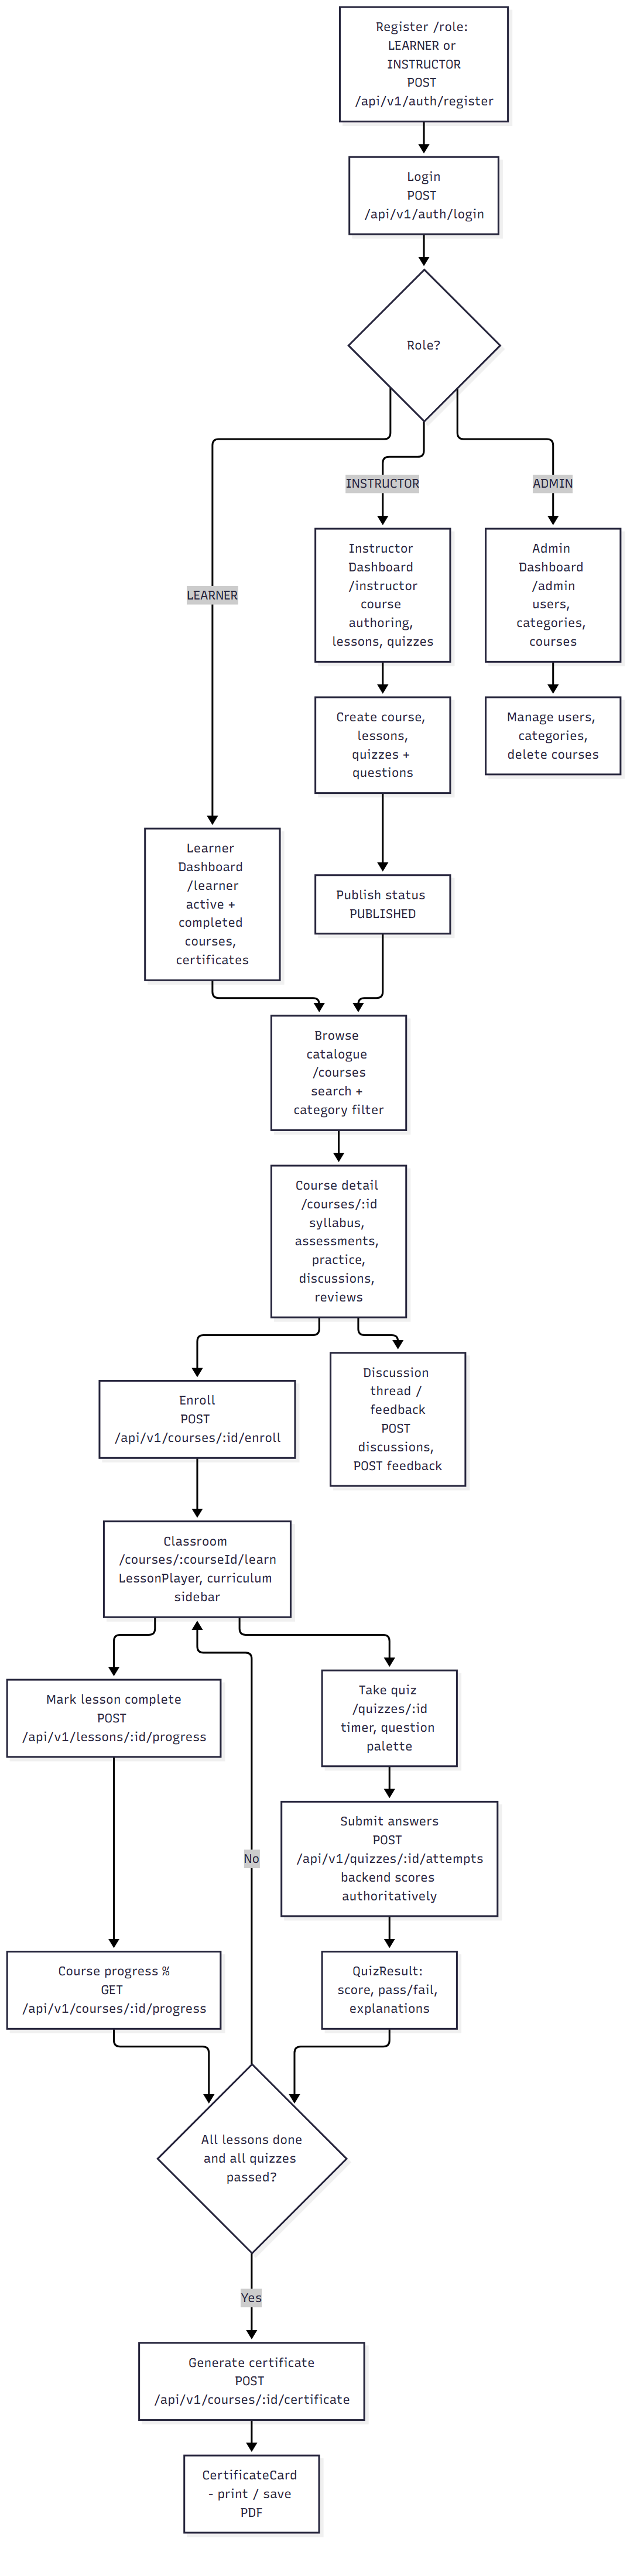
\includegraphics[width=0.86\textwidth]{diagrams/learning-lifecycle.png}
    \caption{Implemented product workflow -- learning lifecycle across the three roles}
    \label{fig:learning-lifecycle}
\end{figure}

\subsection{Use cases}
\status{IMPLEMENTED}

\begin{enumerate}
    \item \textbf{Self-paced learner}: registers, browses the catalogue, enrols, completes lessons in order, passes a timed quiz, and prints a certificate from the dashboard.
    \item \textbf{Instructor content author}: creates a course in draft, adds ordered lessons with video links or reading text, authors a quiz with answer keys, publishes, then reviews learner submissions and scores.
    \item \textbf{Platform administrator}: seeds and curates categories, reviews the user directory, removes courses, and audits all quiz attempts.
    \item \textbf{Practice learner}: opens \code{/practice} or a course's practice tab and solves coding problems inside the embedded OneCompiler editor against a static problem set.
\end{enumerate}

\subsection{Differentiators (repository evidence only)}
\status{IMPLEMENTED}

\begin{itemize}
    \item \textbf{Enforced certificate eligibility}: all lessons completed \emph{and} every quiz passed -- implemented server-side, tested in \pathref{CertificateServiceTest.java}.
    \item \textbf{Course-scoped coding practice}: static, versioned practice problems attached to real course IDs, with starter-code injection via \code{postMessage} into the OneCompiler iframe.
    \item \textbf{Engineering contract as product governance}: \pathref{CONTRACT.md} fixes ownership, API change control, and a Definition of Done -- unusual discipline for a project of this size.
\end{itemize}

\noindent \textbf{Not differentiators, honestly stated:} there is no recommendation engine, no payments, no mobile app, no video hosting, and no analytics -- all explicitly excluded in \pathref{CONTRACT.md} section 5.2.

\subsection{Calls to action present in the UI}
\status{IMPLEMENTED}

Home page (\pathref{frontend/src/pages/HomePage.jsx}): ``Browse all courses'' (primary), ``Join for free'' (logged-out) or ``Go to dashboard'' (logged-in), closing dark CTA band. Auth pages: ``Log in to Edvanta'', ``Create Your Account''. Course pages: ``Enroll Now'' / ``Continue Learning'' (\pathref{frontend/src/components/EnrollmentButton.jsx}). Additional CTA ideas are \status{RECOMMENDED} and intentionally not listed as product copy.

\subsection{Visual identity}
\status{IMPLEMENTED}

Brand gradient \texttt{linear-gradient(90deg, \#fc4c02 0\%, \#ef2cc1 52\%, \#bdbbff 100\%)} rendered by \pathref{frontend/src/components/ui/GradientRibbon.jsx}; black-first UI (\texttt{colorPrimary: \#000000}), mint accent \texttt{\#c8f6f9}, dark canvas \texttt{\#010120}. Full token tables are in Section~\ref{sec:design-system}.

\subsection{SEO keywords and AEO/GEO pointers}
\status{INFERRED (keywords) / IMPLEMENTED (metadata)}

Literal metadata supports the keywords ``LMS'', ``structured courses'', ``assessments'', ``certificates'', ``learn''. \status{RECOMMENDED} additional keyword families (``online learning platform'', ``course management system'') are \emph{not} present in the repository and must be added deliberately -- see Sections~\ref{sec:seo}, \ref{sec:aeo} and \ref{sec:geo} for the gap analysis.

\section{Executive Summary}
\label{sec:executive-summary}

This summary is written for non-technical stakeholders. All statements are traceable to the repository.

\subsection{What the product is}
\status{IMPLEMENTED}

\textbf{Edvanta (Learning Management System)} is a browser-based platform for delivering online courses with assessments, progress tracking and completion certificates. It serves three roles -- learners, instructors and administrators -- through a single responsive web application backed by a secure REST API.

\subsection{The problem it solves}
\status{INFERRED}

Running a complete learning programme requires stitching together content delivery, testing, progress records and credential issuance. This product implements that entire cycle in one system, from account registration through to a printable, uniquely coded certificate.

\subsection{The solution in one paragraph}
\status{IMPLEMENTED}

Learners enrol in courses and work through ordered lessons; the platform records lesson-level progress and derives course completion percentages. Instructors author courses, lessons and multiple-choice quizzes; when a learner submits a quiz the \emph{server} scores it against stored answer keys and persists the attempt. When a learner has completed every lesson of a course and passed every quiz in it, the backend issues a certificate carrying a unique code, the learner's name, the course title and an issue date. Administrators curate categories, review the user directory and moderate the catalogue.

\subsection{Core functionality}
\status{IMPLEMENTED}

\begin{multicols}{2}
\begin{itemize}
    \item JWT authentication with BCrypt password hashing
    \item Role-based access control (learner / instructor / admin)
    \item Course catalogue with search and category filters
    \item Course, lesson and quiz authoring (instructor)
    \item Enrollment with duplicate protection
    \item Lesson player with video/embed and text content
    \item Per-lesson and per-course progress tracking
    \item Timed quizzes, server-side scoring, answer explanations
    \item Threaded course discussions
    \item Course feedback with 1--5 star ratings
    \item Certificate generation with eligibility enforcement
    \item Coding-practice workspace with embedded OneCompiler editor
    \item Admin console for users, categories and courses
    \item Live OpenAPI/Swagger API documentation
\end{itemize}
\end{multicols}

\subsection{Target users}
\status{IMPLEMENTED}

Three account roles are implemented in the database schema (\code{role} column, default \code{LEARNER}; \pathref{database/schema.sql}) and enforced by Spring Security annotations (Section~\ref{sec:authorization}). Typical users: self-paced learners, content-creating instructors, and platform administrators.

\subsection{Technology and architecture}
\status{IMPLEMENTED}

\begin{table}[H]
\centering
\caption{Architecture summary for stakeholders}
\label{tab:exec-arch}
\begin{tabular}{@{}L{3.4cm}L{10.8cm}@{}}
\toprule
\textbf{Concern} & \textbf{Choice} \\
\midrule
Client & React 18 single-page application built with Vite; Ant Design components with Tailwind styling \\
Server & Spring Boot 3.3.4 (Java 21) layered REST API: controller $\rightarrow$ service $\rightarrow$ repository \\
Data store & MySQL 8 with 13 related tables managed through JPA/Hibernate \\
Security & Stateless JSON Web Tokens (24-hour expiry), BCrypt hashing, method-level role checks \\
API style & Versioned JSON REST (\code{/api/v1/...}) wrapped in a consistent \texttt{\{success, message, data\}} envelope \\
Quality tooling & 22 backend tests (JUnit/Mockito/MockMvc), 39 frontend tests (Vitest + Testing Library) \\
\bottomrule
\end{tabular}
\end{table}

\begin{figure}[H]
    \centering
    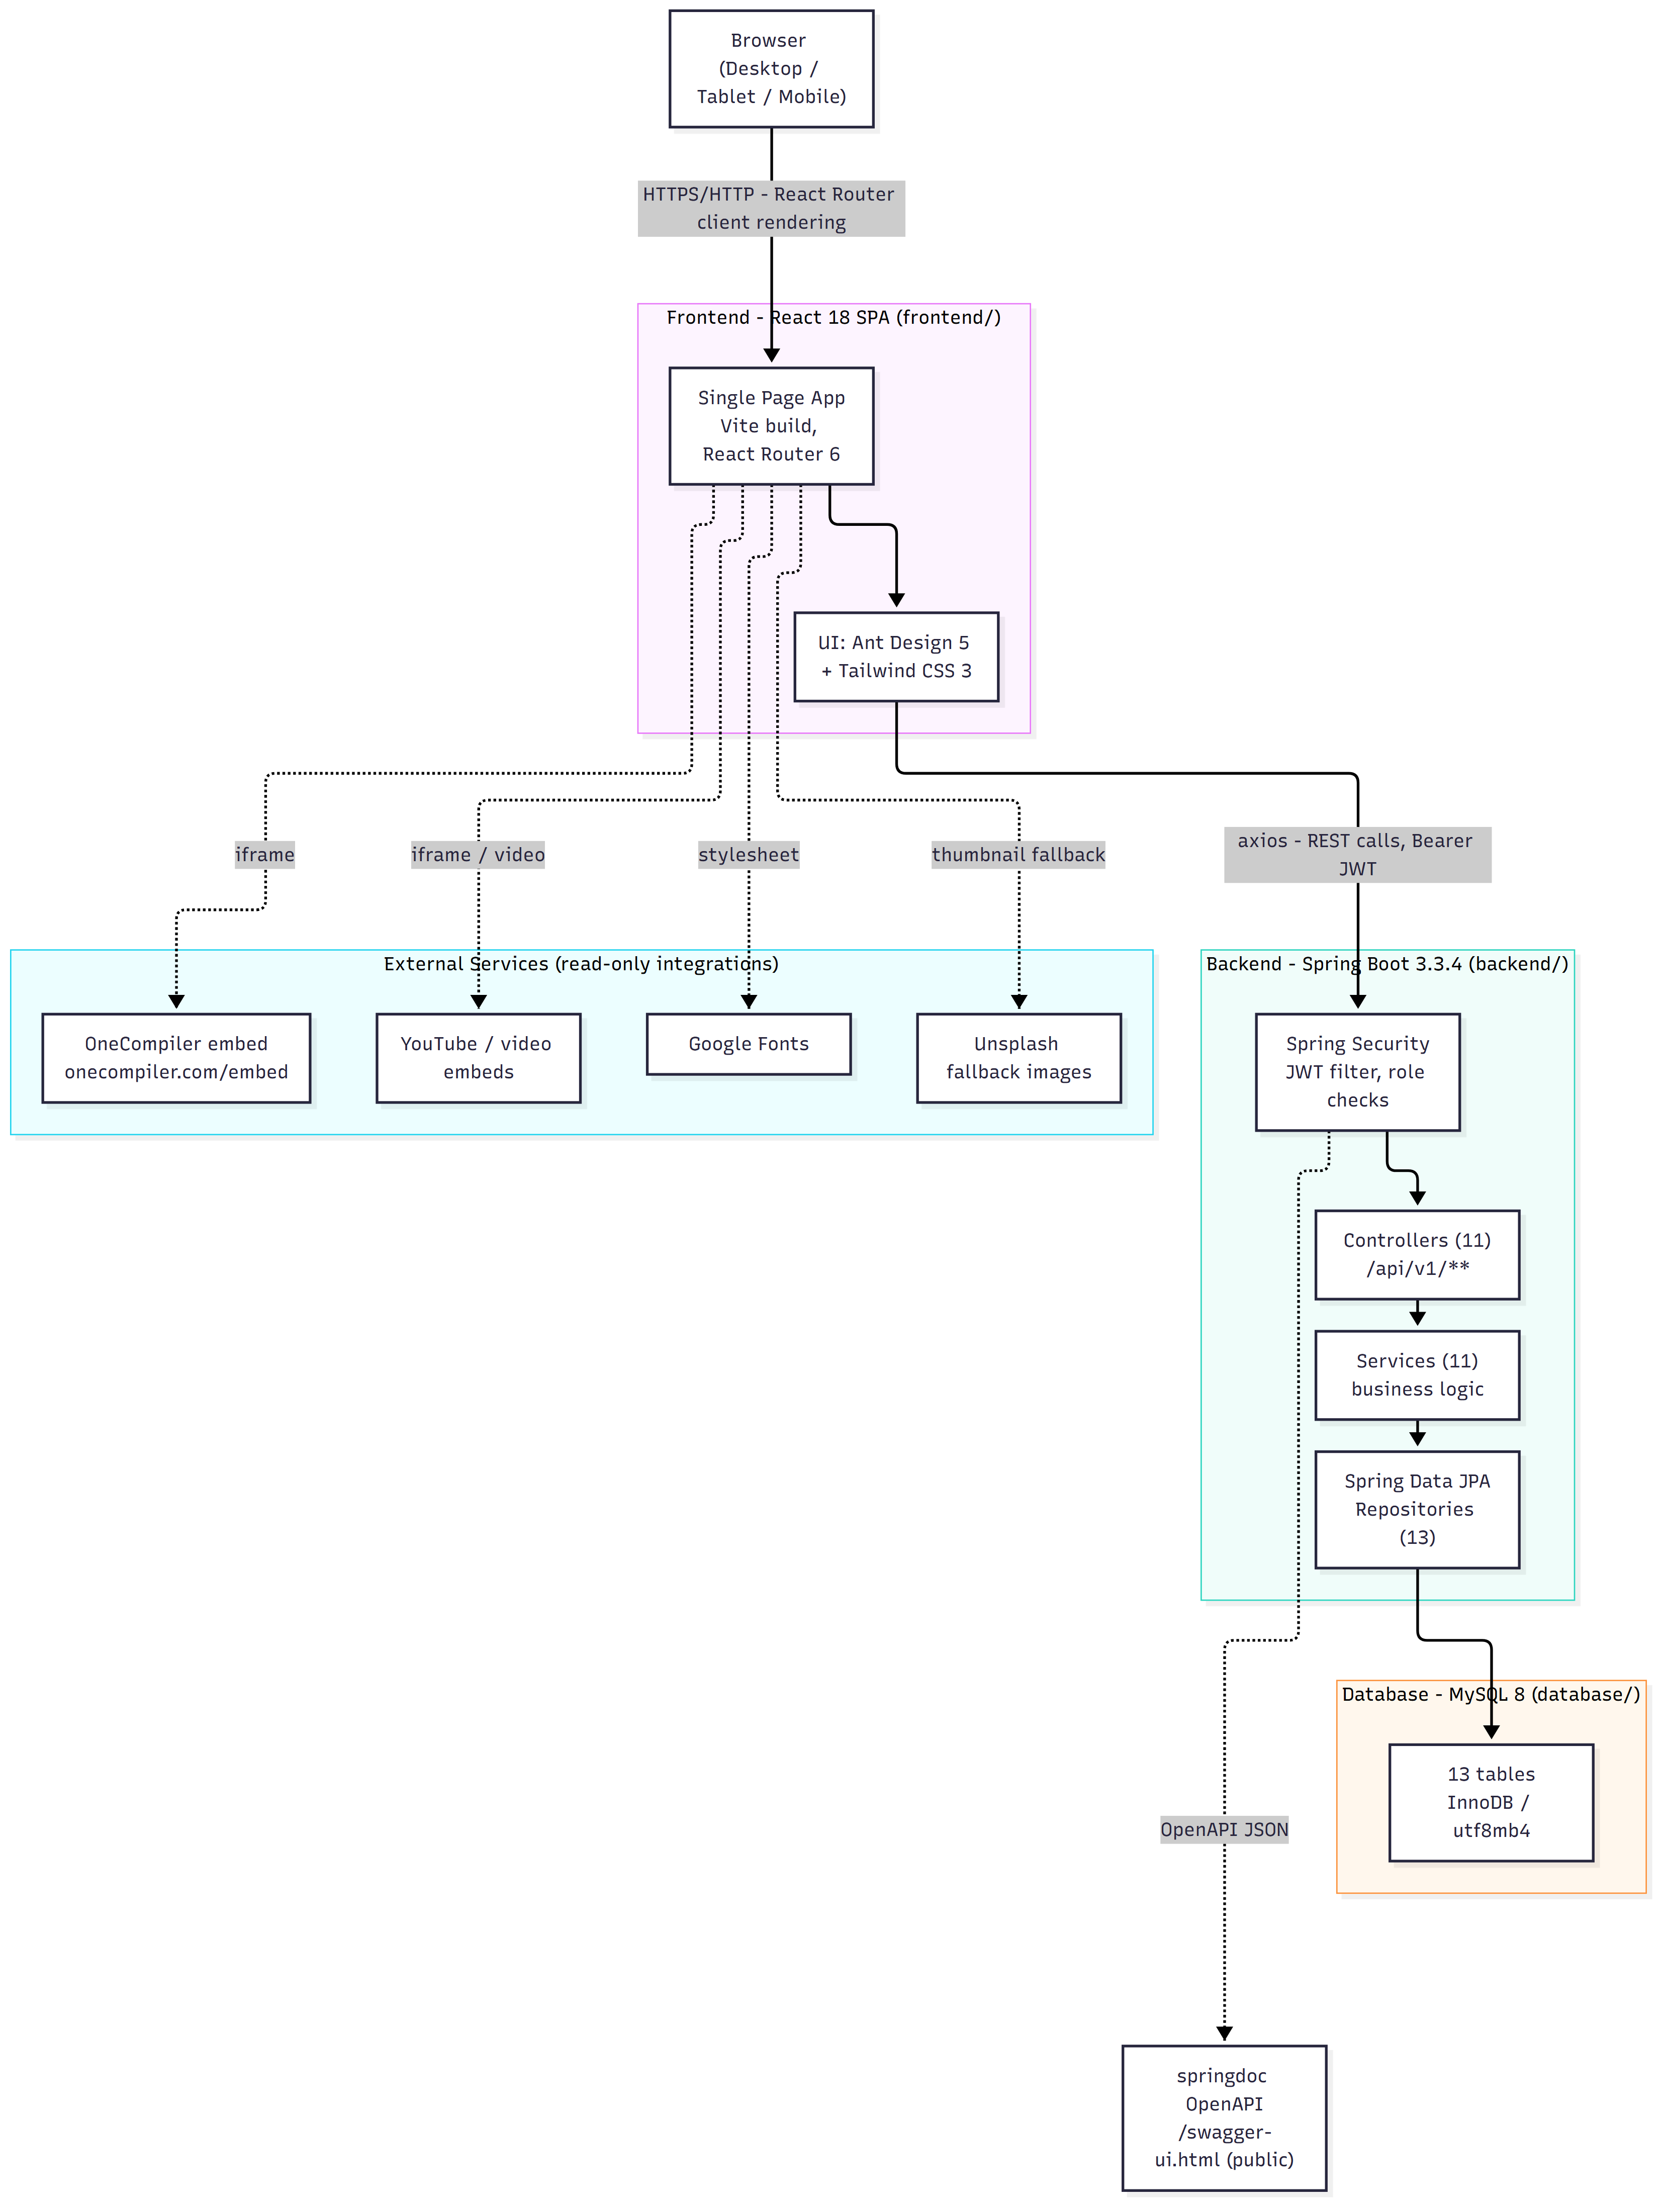
\includegraphics[width=0.72\textwidth]{diagrams/system-architecture.png}
    \caption{System architecture at a glance}
    \label{fig:system-architecture}
\end{figure}

\subsection{Current maturity}
\status{INFERRED}

\begin{itemize}
    \item \textbf{Working:} the end-to-end learning lifecycle passes an automated integration test; the frontend consumes the real API (no mock server); 61 automated tests exist across both tiers.
    \item \textbf{Not yet in place:} CI/CD, production deployment configuration, database migration tooling, licence file, rate limiting, monitoring/alerting, accessibility audit, SEO infrastructure (sitemap/structured data).
    \item \textbf{Repository signals:} 15 commits, active feature branches, contract-driven two-person workflow.
\end{itemize}

\subsection{Key limitations and risks (headline items)}
\status{IMPLEMENTED (verified findings)}

\begin{table}[H]
\centering
\caption{Headline limitations for leadership attention (full detail in Section~\ref{sec:security} and Section~\ref{sec:known-issues})}
\label{tab:exec-risks}
\begin{tabular}{@{}C{2.0cm}L{11.6cm}@{}}
\toprule
\textbf{Severity} & \textbf{Finding (evidence)} \\
\midrule
Critical & Open registration honours a caller-supplied \code{role} field -- an anonymous request can create an ADMIN account (\pathref{backend/src/main/java/com/example/lms/service/AuthService.java}) \\
Critical & Default admin credentials seeded on every fresh database (\code{admin@example.com}/\code{admin123}; \pathref{backend/src/main/java/com/example/lms/config/DataInitializer.java}) \\
High & Default JWT signing secret is committed to source; tokens are forgeable if the environment variable is unset \\
High & CORS allows any origin together with credentials (\pathref{SecurityConfig.java}) \\
Medium & Logout is client-side only -- the token stays valid for 24 hours \\
Medium & No pagination on any list endpoint; dashboard performs sequential per-enrolment requests \\
Medium & Several UI defects: footer links to non-existent routes, dashboard deep links do not switch tabs \\
Low & No CI/CD, no lint configuration, unused dependency (\code{canvas-confetti}) \\
\bottomrule
\end{tabular}
\end{table}

\subsection{Bottom line}
\status{INFERRED}

The repository delivers a credible, tested MVP of the full learn--assess--certify cycle with clear engineering governance (\pathref{CONTRACT.md}). Before any production exposure, the critical and high security findings above must be remediated and a deployment/CI pipeline must be established. These are recommendations, not current capabilities.

\section{Business Requirements Document (BRD)}
\label{sec:brd}

\subsection{Document purpose}
This BRD records the business-level requirements that can be derived from the repository: \pathref{README.md} (objectives, roles), \pathref{CONTRACT.md} (scope, exclusions, Definition of Done) and the implemented behaviour of the code. No revenue model, customer list, market data or KPI targets exist anywhere in the repository; such items are marked \status{UNKNOWN}.

\subsection{Business problem}
\status{INFERRED (from README objectives and implemented scope)}

Educational content delivery, learner assessment, progress record-keeping and credential issuance are fragmented across tools. The repository exists to provide a single platform covering the complete cycle:

\begin{center}
\texttt{Registration $\rightarrow$ Discovery $\rightarrow$ Enrollment $\rightarrow$ Learning $\rightarrow$ Assessment $\rightarrow$ Evaluation $\rightarrow$ Completion $\rightarrow$ Certificate}
\end{center}

\noindent This lifecycle is stated verbatim in \pathref{README.md} and \pathref{CONTRACT.md} section~1 and implemented in code.

\subsection{Business objectives}
\status{IMPLEMENTED (objectives as declared in README.md; implementation status verified below)}

\begin{table}[H]
\centering
\caption{Declared objectives versus implementation status}
\label{tab:brd-objectives}
\begin{tabular}{@{}L{7.6cm}C{3.0cm}L{3.0cm}@{}}
\toprule
\textbf{Objective (README)} & \textbf{Status} & \textbf{Evidence} \\
\midrule
Centralised platform for online learning & IMPLEMENTED & Single SPA + API + database \\
User registration and enrolment & IMPLEMENTED & AuthController, EnrollmentService \\
Structured course content and materials & IMPLEMENTED & Lesson entity (URL + rich text) \\
Learner progress tracking & IMPLEMENTED & ProgressService, progress table \\
Online assessments and quizzes & IMPLEMENTED & QuizService, quiz tables \\
Performance recording and display & IMPLEMENTED & QuizAttempt, QuizResult UI \\
Communication around courses & IMPLEMENTED & DiscussionService, DiscussionList \\
Instructor content management tools & IMPLEMENTED & InstructorDashboard \\
Centralised system administration & IMPLEMENTED & AdminDashboard, UserController \\
Certificates after completion & IMPLEMENTED & CertificateService (eligibility enforced) \\
Secure authentication and RBAC & IMPLEMENTED & Spring Security + \code{@PreAuthorize} \\
\bottomrule
\end{tabular}
\end{table}

\subsection{Stakeholders}
\status{IMPLEMENTED (roles) / INFERRED (interest)}

\begin{table}[H]
\centering
\caption{Stakeholder map}
\label{tab:stakeholders}
\begin{tabular}{@{}L{3.6cm}L{4.4cm}L{5.6cm}@{}}
\toprule
\textbf{Stakeholder} & \textbf{Role in project} & \textbf{Interest} \\
\midrule
Learner (end user) & Platform user & Complete courses, pass assessments, hold certificates \\
Instructor (content owner) & Platform user & Author and publish content, monitor submissions \\
Administrator & Platform operator & Curate catalogue, manage users, enforce policy \\
Frontend workstream (Jay) & Code owner per \pathref{CONTRACT.md} & UI/UX quality, frontend tests, integration \\
Backend workstream (Ali) & Code owner per \pathref{CONTRACT.md} & API contract, security, schema, backend tests \\
AI coding agents & Assisted contributors & Must obey \pathref{CONTRACT.md} section 26 rules \\
\bottomrule
\end{tabular}
\end{table}

\subsection{User groups}
\status{IMPLEMENTED}

The three user groups map directly to the \code{users.role} column (\pathref{database/schema.sql}) and to route-level restrictions in \pathref{frontend/src/routes/AppRoutes.jsx} plus server-side rules in \pathref{backend/src/main/java/com/example/lms/config/SecurityConfig.java}. Their permissions are tabulated in Section~\ref{sec:authorization}.

\subsection{Business processes}
\status{IMPLEMENTED}

\begin{enumerate}
    \item \textbf{Learner acquisition:} register $\rightarrow$ verify email-uniqueness $\rightarrow$ receive JWT $\rightarrow$ browse $\rightarrow$ enrol.
    \item \textbf{Content publishing:} instructor creates course (DRAFT) $\rightarrow$ adds ordered lessons $\rightarrow$ authors quiz + questions $\rightarrow$ sets status PUBLISHED $\rightarrow$ course becomes discoverable.
    \item \textbf{Learning delivery:} enrol $\rightarrow$ open classroom $\rightarrow$ consume lesson (video/embed/text) $\rightarrow$ mark complete $\rightarrow$ progress recomputed.
    \item \textbf{Assessment:} open quiz $\rightarrow$ answer under time limit $\rightarrow$ submit $\rightarrow$ server scores $\rightarrow$ result persisted and displayed with explanations.
    \item \textbf{Credentialing:} all lessons complete + all quizzes passed $\rightarrow$ backend issues certificate $\rightarrow$ learner prints/saves from dashboard.
    \item \textbf{Quality loop:} enrolled learners post discussions and one feedback rating per course; instructors view attempt results.
\end{enumerate}

\subsection{Business requirements}
\status{IMPLEMENTED unless stated otherwise}

\begin{table}[H]
\centering
\caption{Business requirements register}
\label{tab:brd-requirements}
\begin{tabular}{@{}C{1.4cm}L{9.0cm}C{3.6cm}@{}}
\toprule
\textbf{ID} & \textbf{Requirement} & \textbf{Status} \\
\midrule
BR-01 & The platform must serve learner, instructor and administrator roles in one system & IMPLEMENTED \\
BR-02 & Learners must be able to self-register and immediately receive an authenticated session & IMPLEMENTED \\
BR-03 & Only authorised users may create or modify courses and lessons & IMPLEMENTED \\
BR-04 & Assessment results must be computed by the server, never trusted from the client & IMPLEMENTED \\
BR-05 & Certificates must only be issued when completion requirements are met & IMPLEMENTED \\
BR-06 & The system must prevent duplicate active enrolments and duplicate feedback & IMPLEMENTED \\
BR-07 & The platform must be usable on desktop, tablet and mobile browsers & IMPLEMENTED (responsive classes; no formal audit) \\
BR-08 & The product must be documented for engineering hand-over & IMPLEMENTED (this document) \\
BR-09 & Payment, subscriptions and live classes are out of scope for v1.0 & IMPLEMENTED (excluded in \pathref{CONTRACT.md} 5.2) \\
BR-10 & Business revenue, market-share or growth targets & UNKNOWN (not present in repository) \\
\bottomrule
\end{tabular}
\end{table}

\subsection{Expected outcomes}
\status{IMPLEMENTED (product outcomes) / UNKNOWN (business outcomes)}

\begin{itemize}
    \item A learner can go from registration to a printable certificate without human intervention -- proven by \pathref{backend/src/test/java/com/example/lms/integration/LmsIntegrationTest.java}.
    \item An instructor can publish a course with lessons and a quiz entirely through the UI.
    \item An administrator can curate categories and review platform users and courses.
    \item \textbf{Business} outcomes (enrolment volume, completion rates, revenue) are \status{UNKNOWN} -- the repository contains no analytics, telemetry or reporting pipeline.
\end{itemize}

\subsection{Success metrics}
\status{UNKNOWN}

No instrumentation for business metrics exists in the repository (no analytics package in \pathref{frontend/package.json}, no metrics/actuator dependency in \pathref{backend/pom.xml}, no reporting tables in \pathref{database/schema.sql}). The only measurable quality signals available today are:

\begin{table}[H]
\centering
\caption{Available (engineering) success signals}
\label{tab:brd-metrics}
\begin{tabular}{@{}L{7.4cm}L{4.0cm}L{2.4cm}@{}}
\toprule
\textbf{Signal} & \textbf{Value} & \textbf{Status} \\
\midrule
Backend automated tests & 22 test methods across 10 classes & IMPLEMENTED \\
Frontend automated tests & 39 test methods across 8 files & IMPLEMENTED \\
End-to-end lifecycle test & 1 full-stack integration scenario & IMPLEMENTED \\
Coverage measurement & none configured (no JaCoCo, no coverage script) & NOT PRESENT \\
\bottomrule
\end{tabular}
\end{table}

\subsection{Constraints}
\status{IMPLEMENTED (declared in repository documents)}

\begin{itemize}
    \item Two-person workstream ownership with strict directory boundaries (\pathref{CONTRACT.md} sections 3 and 27).
    \item Fixed technology baseline; major replacements require both contributors' agreement (\pathref{CONTRACT.md} section 2).
    \item Feature work must not alter APIs or schema without coordinated change management (sections 29--30).
    \item Frontend route guards are explicitly \emph{not} security boundaries -- enforcement is a backend duty (section 13).
    \item No licence file exists despite an MIT claim in \pathref{README.md} (legal constraint gap).
\end{itemize}

\subsection{Assumptions}
\status{INFERRED}

\begin{enumerate}
    \item MySQL is available to developers at \code{localhost:3306} with credentials supplied via environment (per \pathref{.env.example}).
    \item The application is single-tenant (no multi-tenant requirement appears anywhere).
    \item English is the only locale (no i18n files exist).
    \item HTTPS termination, if any, is handled outside the repository (no TLS configuration exists).
\end{enumerate}

\subsection{Risks}
\status{IMPLEMENTED (verified conditions)}

\begin{table}[H]
\centering
\caption{Business-facing risks with repository evidence}
\label{tab:brd-risks}
\begin{tabular}{@{}C{1.6cm}L{12.2cm}@{}}
\toprule
\textbf{Severity} & \textbf{Risk} \\
\midrule
Critical & Self-registration can mint ADMIN accounts (\code{role} honoured in \pathref{backend/src/main/java/com/example/lms/service/AuthService.java}) -- undermines the entire role model \\
Critical & Default admin/instructor/learner credentials are seeded on empty databases in any environment \\
High & Committed default JWT secret allows token forgery when \code{JWT_SECRET} is unset \\
High & Wildcard CORS with credentials exposes authenticated APIs to any origin \\
Medium & No CI/CD means regressions are only caught by developers remembering to run tests \\
Medium & No analytics means business success cannot be measured \\
Low & MIT licence claimed but LICENSE file missing -- redistribution terms unclear \\
\bottomrule
\end{tabular}
\end{table}

\section{Product Requirements Document (PRD)}
\label{sec:prd}

\subsection{Product vision}
\status{INFERRED (synthesised from README.md and CONTRACT.md)}

Give every learner, instructor and administrator one secure, self-service platform where the full learning lifecycle -- discover, enrol, learn, prove, certify -- works end-to-end without operational overhead.

\subsection{Problem statement}
\status{INFERRED}

Learners need a trustworthy path from course discovery to a verifiable credential; instructors need authoring and monitoring tools; administrators need catalogue and user control. Today these are separate activities. The product solves them as one integrated flow.

\subsection{Goals and objectives}
\status{IMPLEMENTED (goals declared in repository) / INFERRED (framing)}

\begin{table}[H]
\centering
\caption{PRD goals mapped to implemented capability}
\label{tab:prd-goals}
\begin{tabular}{@{}C{1.4cm}L{8.4cm}L{4.4cm}@{}}
\toprule
\textbf{ID} & \textbf{Goal} & \textbf{Implementation evidence} \\
\midrule
G1 & Secure, role-aware access for three personas & \pathref{backend/src/main/java/com/example/lms/config/SecurityConfig.java} + ProtectedRoute \\
G2 & Full course catalogue with search/filter & CourseController + CourseCatalogPage \\
G3 & Structured learning with progress visibility & LessonPlayer, ProgressBar, ProgressService \\
G4 & Authoritative assessment & QuizService scoring, QuizResult review UI \\
G5 & Evidence of completion & CertificateService eligibility + CertificateCard \\
G6 & Engagement: discussion and feedback & DiscussionService, FeedbackService \\
G7 & Self-service authoring for instructors & InstructorDashboard (course/lesson/quiz modals) \\
G8 & Extensible practice layer & \pathref{frontend/src/components/practice/} + local dataset \\
G9 & Contract-driven, tested delivery & \pathref{CONTRACT.md}, 61 automated tests \\
\bottomrule
\end{tabular}
\end{table}

\subsection{Personas}
Covered in Section~\ref{sec:project-description} (personas inferred from seeded accounts; \status{INFERRED}).

\subsection{User stories}
\status{IMPLEMENTED (stories exercised by existing code and tests)}

\begin{table}[H]
\centering
\caption{Primary user stories}
\label{tab:user-stories}
\begin{tabular}{@{}C{1.3cm}L{9.2cm}L{3.6cm}@{}}
\toprule
\textbf{ID} & \textbf{Story} & \textbf{Covered by} \\
\midrule
US-01 & As a visitor I can register and log in so that I can use the platform & AuthControllerTest \\
US-02 & As a learner I can browse and search the catalogue without logging in & public GET \code{/api/v1/courses} \\
US-03 & As a learner I can enrol in a course exactly once & EnrollmentServiceTest \\
US-04 & As a learner I can mark lessons complete and see course progress & ProgressServiceTest \\
US-05 & As a learner I can take a quiz under a time limit and see my score & QuizServiceTest, quiz.test.jsx \\
US-06 & As a learner I can generate a certificate when I complete a course & CertificateServiceTest \\
US-07 & As a learner I can discuss a course and leave one rating/feedback & social\_cert.test.jsx \\
US-08 & As an instructor I can create, edit, publish and delete my courses & CourseServiceTest, InstructorDashboard \\
US-09 & As an instructor I can author quizzes with questions and answer keys & InstructorDashboard quiz modal \\
US-10 & As an instructor I can view learner submissions for my quizzes & QuizService results scoping \\
US-11 & As an admin I can manage categories and view all users & CategoryController, UserController \\
US-12 & As any user I can update my profile (name, bio, avatar) & ProfilePage + UserService \\
\bottomrule
\end{tabular}
\end{table}

\subsection{Use cases}
Covered in Section~\ref{sec:project-description} (use cases UC-1 to UC-4).

\subsection{Features and functional requirements}
\status{IMPLEMENTED}

The authoritative feature list with acceptance-relevant detail is maintained in Section~\ref{sec:functional-requirements}. Feature inventory for product readers is in Section~\ref{sec:project-description}.

\subsection{Acceptance criteria}
\status{IMPLEMENTED (Definition of Done as written in CONTRACT.md section 32)}

The repository's own acceptance gate is the Definition of Done. Summarised (full checklist in \pathref{CONTRACT.md}):

\begin{itemize}
    \item \textbf{Authentication:} register/login/logout work; passwords hashed; JWT works; protected routes and role authorisation work; invalid authentication handled.
    \item \textbf{Courses:} CRUD works; ownership/permissions enforced.
    \item \textbf{Enrollment:} learner can enrol; duplicates prevented; unauthorised actions rejected.
    \item \textbf{Learning:} lessons load; completion recorded; progress persisted and reflected in the UI.
    \item \textbf{Assessments:} quiz loads; answers submitted; \emph{backend} calculates authoritative score; results persisted and visible.
    \item \textbf{Discussions/Feedback:} creation, retrieval, replies, validation and unauthorised-modification rejection work.
    \item \textbf{Certificates:} requirements validated; correct learner/course data; downloadable.
    \item \textbf{Frontend:} all pages implemented; loading/empty/error states exist; forms validate; responsive layout; tests pass; production build succeeds.
    \item \textbf{Integration:} frontend connects to the real backend; no required feature depends on temporary mock data.
\end{itemize}

\noindent \textbf{Gap versus gate:} the practice module ships with static data by explicit design (\pathref{frontend/src/data/practiceData.js} header comment), and \pathref{CONTRACT.md} allows mocks only during isolated frontend development. \status{KNOWN DEVIATION}

\subsection{Success metrics}
\status{UNKNOWN}

No product analytics exist (see Section~\ref{sec:brd}). \status{RECOMMENDED} metrics to instrument before launch: registration$\rightarrow$enrolment conversion, course completion rate, quiz pass rate, certificate issue rate -- none of these can currently be measured.

\subsection{Constraints}
\status{IMPLEMENTED}

\begin{itemize}
    \item v1.0 scope boundaries (excluded: payments, streaming, mobile apps, AI features, SSO, multi-tenancy) -- \pathref{CONTRACT.md} section 5.2.
    \item Two-workstream ownership; cross-boundary changes require coordination (sections 27, 29--31).
    \item Single language (English), single database, single deployment target implied by configuration.
\end{itemize}

\subsection{Dependencies}
\status{IMPLEMENTED}

\begin{table}[H]
\centering
\caption{External and internal dependencies}
\label{tab:prd-dependencies}
\begin{tabular}{@{}L{5.0cm}L{7.6cm}C{2.2cm}@{}}
\toprule
\textbf{Dependency} & \textbf{Use} & \textbf{Status} \\
\midrule
MySQL 8 & Primary data store & Required at runtime \\
Node.js + npm & Frontend build/test & Required at build time \\
Java 21 + Maven & Backend build (Maven wrapper 3.9.9 included) & Required at build time \\
Google Fonts (Inter, JetBrains Mono) & Typography (\pathref{frontend/index.html}) & Runtime CDN call \\
OneCompiler embed & Coding-practice editor iframe & Runtime third-party \\
YouTube embed URLs & Lesson video players & Content-supplied \\
Unsplash images & Fallback thumbnails (hardcoded URLs) & Runtime third-party \\
\bottomrule
\end{tabular}
\end{table}

\subsection{Risks}
Covered in Section~\ref{sec:brd} (risks) and Section~\ref{sec:known-issues} (defects).

\subsection{Future scope}
\status{IMPLEMENTED (as declared) / NOT IMPLEMENTED (as content)}

\pathref{README.md} publishes a four-phase roadmap: Phase 1 (core LMS) is marked complete; Phases 2--4 (discussions/feedback/notifications/analytics, instructor platform, advanced platform incl. password recovery, CI/CD, monitoring) are unchecked. Note that discussions and feedback \emph{are} already implemented while listed as Phase~2 -- the README roadmap has drifted from the code. The reconciled roadmap is Section~\ref{sec:roadmap}.

\section{Functional Requirements}
\label{sec:functional-requirements}

Each requirement is traceable to implemented code. \status{IMPLEMENTED} means behaviour was verified in source; \status{RECOMMENDED} marks capabilities that do not exist and are suggested, not promised.

\subsection{Authentication and account management (FR-AUTH)}
\begin{table}[H]
\centering
\caption{Functional requirements -- authentication}
\label{tab:fr-auth}
\begin{tabular}{@{}C{1.5cm}L{8.6cm}L{3.9cm}@{}}
\toprule
\textbf{ID} & \textbf{Requirement} & \textbf{Evidence} \\
\midrule
FR-AUTH-01 & The system shall allow self-registration with name, email, password and role & \code{POST /api/v1/auth/register} \\
FR-AUTH-02 & Passwords shall be stored only as BCrypt hashes & \code{BCryptPasswordEncoder} in SecurityConfig \\
FR-AUTH-03 & Email uniqueness must be enforced at registration (409 on duplicate) & AuthService \code{existsByEmail} \\
FR-AUTH-04 & Password policy: minimum 6, maximum 100 characters & \code{@Size} on RegisterRequest \\
FR-AUTH-05 & Successful authentication returns a signed JWT (24 h) plus the user profile & AuthResponse \\
FR-AUTH-06 & Login failures return 401 \code{UNAUTHORIZED} with generic message & AuthService + GlobalExceptionHandler \\
FR-AUTH-07 & Subsequent requests authenticate via \code{Authorization: Bearer} header & JwtAuthenticationFilter \\
FR-AUTH-08 & Profile update (name, bio, avatar URL; optional password) for self or admin & UserService.updateUser \\
FR-AUTH-09 & \emph{Client} logout clears stored token and calls \code{POST /auth/logout} & AuthContext.logout \\
FR-AUTH-10 & Server-side logout must invalidate the token & \status{RECOMMENDED} (not implemented -- endpoint is a no-op) \\
\bottomrule
\end{tabular}
\end{table}

\subsection{Course management (FR-COURSE)}
\begin{table}[H]
\centering
\caption{Functional requirements -- courses}
\label{tab:fr-course}
\begin{tabular}{@{}C{1.5cm}L{8.6cm}L{3.9cm}@{}}
\toprule
\textbf{ID} & \textbf{Requirement} & \textbf{Evidence} \\
\midrule
FR-CRS-01 & List courses with optional \code{search}, \code{categoryId}, \code{status}, \code{instructorId} filters & CourseController GET \\
FR-CRS-02 & Retrieve a single course incl.\ computed \code{totalLessons}, \code{totalEnrolled} & CourseService.mapToCourseResponse \\
FR-CRS-03 & Create a course restricted to INSTRUCTOR/ADMIN (403 otherwise) & \code{@PreAuthorize} on POST \\
FR-CRS-04 & Update/delete restricted to admin or the owning instructor & \code{validateCourseOwnership} \\
FR-CRS-05 & Course status lifecycle: DRAFT, PUBLISHED, ARCHIVED & \code{Course.Status} enum \\
FR-CRS-06 & Course fields: title, description, category, thumbnail URL, instructor & CourseCreateRequest \\
FR-CRS-07 & Category CRUD restricted to ADMIN; duplicate names rejected (409) & CategoryController/Service \\
FR-CRS-08 & Public (unauthenticated) read access to course list and detail & SecurityConfig permitAll GET \\
\bottomrule
\end{tabular}
\end{table}

\subsection{Lessons and learning delivery (FR-LESSON)}
\begin{table}[H]
\centering
\caption{Functional requirements -- lessons and player}
\label{tab:fr-lesson}
\begin{tabular}{@{}C{1.5cm}L{8.6cm}L{3.9cm}@{}}
\toprule
\textbf{ID} & \textbf{Requirement} & \textbf{Evidence} \\
\midrule
FR-LSN-01 & Lessons belong to a course with explicit \code{orderIndex} and \code{durationMinutes} & Lesson entity \\
FR-LSN-02 & Lesson content: external/video URL, embeddable media, or long-form text & LessonPlayer media detection \\
FR-LSN-03 & Lesson CRUD restricted to instructor-owner/admin & LessonController \code{@PreAuthorize} \\
FR-LSN-04 & New lessons default to the next order index & LessonService.createLesson \\
FR-LSN-05 & Learner can mark a lesson complete (100\%) with watch-time seconds & ProgressController POST/PATCH \\
FR-LSN-06 & Classroom shows curriculum sidebar with completion state and lesson navigation & LearningPage \\
FR-LSN-07 & Video URLs (YouTube/Vimeo/\code{.mp4}) are converted to embeddable players & \code{getEmbedUrl} in LessonPlayer \\
\bottomrule
\end{tabular}
\end{table}

\subsection{Enrollment and progress (FR-ENR)}
\begin{table}[H]
\centering
\caption{Functional requirements -- enrollment and progress}
\label{tab:fr-enroll}
\begin{tabular}{@{}C{1.5cm}L{8.6cm}L{3.9cm}@{}}
\toprule
\textbf{ID} & \textbf{Requirement} & \textbf{Evidence} \\
\midrule
FR-ENR-01 & Learner enrols in a course; duplicate active enrolment returns 409 & EnrollmentService.enroll \\
FR-ENR-02 & Unenrolment is a soft drop (status DROPPED), rows are retained & EnrollmentService.unenroll \\
FR-ENR-03 & Only self or ADMIN may list a user's enrolments (403 otherwise) & EnrollmentService.getUserEnrollments \\
FR-ENR-04 & Instructors are blocked from enrolling as learners in the UI & EnrollmentButton guard \\
FR-PRG-01 & Progress is stored per user+lesson with unique constraint & \code{uk_user_lesson_progress} \\
FR-PRG-02 & Course progress \% is computed as completed/total lessons (2 dp) & ProgressService.getCourseProgress \\
FR-PRG-03 & Completing all lessons auto-marks the enrolment COMPLETED & \code{checkAndUpdateCourseCompletion} \\
FR-PRG-04 & Dashboard distinguishes active vs completed enrolments & LearnerDashboard \\
\bottomrule
\end{tabular}
\end{table}

\subsection{Assessments (FR-QUIZ)}
\begin{table}[H]
\centering
\caption{Functional requirements -- quizzes}
\label{tab:fr-quiz}
\begin{tabular}{@{}C{1.5cm}L{8.6cm}L{3.9cm}@{}}
\toprule
\textbf{ID} & \textbf{Requirement} & \textbf{Evidence} \\
\midrule
FR-QIZ-01 & Quizzes belong to a course with passing score (default 70\%) and time limit (default 30 min) & Quiz entity/service defaults \\
FR-QIZ-02 & Questions have four options, a correct option (A--D), points (default 10) and an explanation & Question entity \\
FR-QIZ-03 & Learners receive questions \emph{without} correct answers; instructors/admins with them & \code{includeAnswers} flag in QuizService \\
FR-QIZ-04 & Quiz authoring (create/update/delete) restricted to instructor-owner/admin & \code{@PreAuthorize} + ownership check \\
FR-QIZ-05 & Submission is scored server-side: \code{earned/possible x 100}, pass if $\geq$ passing score & QuizService.submitQuiz \\
FR-QIZ-06 & Each attempt persists score, total points, passed flag and per-answer correctness & quiz\_attempt tables \\
FR-QIZ-07 & Result view shows per-question explanations and correct answers & QuizResult component \\
FR-QIZ-08 & Instructors see attempts for their own quizzes; admins see all & \code{getQuizResults} scoping \\
FR-QIZ-09 & Empty quizzes cannot be submitted (400) & \code{no questions to evaluate} check \\
FR-QIZ-10 & Scoring denominator shall include unanswered questions & \status{RECOMMENDED} (current code counts only submitted answers) \\
\bottomrule
\end{tabular}
\end{table}

\subsection{Social features (FR-SOC) and certificates (FR-CERT)}
\begin{table}[H]
\centering
\caption{Functional requirements -- discussions, feedback, certificates}
\label{tab:fr-social}
\begin{tabular}{@{}C{1.5cm}L{8.6cm}L{3.9cm}@{}}
\toprule
\textbf{ID} & \textbf{Requirement} & \textbf{Evidence} \\
\midrule
FR-SOC-01 & Threaded course discussions (top-level posts + nested replies, depth-limited in UI) & Discussion entity self-reference \\
FR-SOC-02 & Only the author or ADMIN may delete a discussion (403 otherwise) & DiscussionService.deleteDiscussion \\
FR-SOC-03 & Feedback requires enrolment; one rating (1--5) per user/course; updates allowed & FeedbackService checks \\
FR-SOC-04 & Course review page shows average rating and per-star distribution & FeedbackForm \\
FR-CERT-01 & Certificate generation requires enrolment & CertificateService eligibility check \\
FR-CERT-02 & All lessons of the course must be completed (when lessons exist) & \code{completedLessons < totalLessons} guard \\
FR-CERT-03 & Every quiz in the course must have a passed attempt & \code{existsByQuizIdAndUserIdAndPassedTrue} \\
FR-CERT-04 & Unique certificate code (\code{LMS-XXXXXXXX-NNNN}) + issue date + learner/course data & CertificateService \\
FR-CERT-05 & Generation is idempotent -- existing certificate is returned & \code{orphan} check first \\
FR-CERT-06 & Learner can print/save the certificate as PDF from the browser & CertificateCard \code{window.print()} \\
FR-CERT-07 & Public certificate verification endpoint & \status{RECOMMENDED} (README Phase 4 item; not implemented) \\
\bottomrule
\end{tabular}
\end{table}

\subsection{Administration (FR-ADM) and practice (FR-PRA)}
\begin{table}[H]
\centering
\caption{Functional requirements -- administration and practice module}
\label{tab:fr-admin}
\begin{tabular}{@{}C{1.5cm}L{8.6cm}L{3.9cm}@{}}
\toprule
\textbf{ID} & \textbf{Requirement} & \textbf{Evidence} \\
\midrule
FR-ADM-01 & List all users (ADMIN only, enforced server-side) & \code{GET /api/v1/users} \code{@PreAuthorize} \\
FR-ADM-02 & Admin console with KPI tiles, user directory, category CRUD, course moderation & AdminDashboard \\
FR-ADM-03 & Role changes only performed by ADMIN & UserService.updateUser \\
FR-ADM-04 & Bootstrap data: 4 default categories and 3 demo accounts on empty DB & DataInitializer \\
FR-PRA-01 & Global practice workspace listing 7 problems (3 languages) with difficulty badges & PracticePage + practiceData.js \\
FR-PRA-02 & Course-scoped practice tab for problems attached to a course & CoursePracticeTab \\
FR-PRA-03 & Embedded OneCompiler editor with starter-code injection via \code{postMessage} & OneCompilerEditor \\
FR-PRA-04 & Practice data served from a backend API & \status{RECOMMENDED} (explicitly local today; single-file swap designed in) \\
\bottomrule
\end{tabular}
\end{table}

\subsection{Cross-cutting functional behaviour}
\begin{itemize}
    \item \textbf{Consistent envelopes:} every success body is \texttt{\{success, message, data\}}; every error body is \texttt{\{error: \{code, message, details?\}\}} (\pathref{backend/src/main/java/com/example/lms/dto/response/ApiResponse.java}, \pathref{ErrorResponse.java}).
    \item \textbf{Validation:} Bean Validation (\code{@Valid}) on all request DTOs; field errors aggregated into \code{VALIDATION_ERROR} with per-field details.
    \item \textbf{UI states:} every major page implements loading / success / empty / error / retry states as mandated by \pathref{CONTRACT.md} section 16 (LoadingState, ErrorState, EmptyState components).
    \item \textbf{Public reads:} unauthenticated users can browse courses and categories; everything else requires a token (SecurityConfig).
\end{itemize}

\section{Non-Functional Requirements}
\label{sec:non-functional-requirements}

Non-functional requirements (NFRs) are assessed against the repository. \status{IMPLEMENTED} = satisfied by code; \status{PARTIAL} = partially satisfied with evidence; \status{NOT IMPLEMENTED} = no evidence; \status{UNKNOWN} = cannot be determined from the repository.

\subsection{Security NFRs}
\begin{table}[H]
\centering
\caption{Security non-functional requirements}
\label{tab:nfr-security}
\begin{tabular}{@{}C{1.4cm}L{8.8cm}L{3.8cm}@{}}
\toprule
\textbf{ID} & \textbf{Requirement} & \textbf{Assessment} \\
\midrule
NFR-SEC-01 & Passwords stored hashed (never plaintext) & IMPLEMENTED -- BCrypt \\
NFR-SEC-02 & Authentication via short-lived signed tokens & PARTIAL -- 24 h JWT, no rotation/revocation \\
NFR-SEC-03 & Authorisation enforced server-side on every protected operation & PARTIAL -- method security present; several service-level gaps (Section~\ref{sec:security}) \\
NFR-SEC-04 & Secrets supplied via environment, never committed & NOT IMPLEMENTED -- default JWT secret and seed credentials committed \\
NFR-SEC-05 & Safe CORS configuration & NOT IMPLEMENTED -- wildcard origin + credentials \\
NFR-SEC-06 & SQL injection prevention & IMPLEMENTED -- JPA parameterised queries, no string-concatenated SQL found \\
NFR-SEC-07 & XSS prevention & IMPLEMENTED (client) -- React escapes output; no \code{dangerouslySetInnerHTML} found \\
NFR-SEC-08 & CSRF protection & BY DESIGN N/A -- stateless JWT, CSRF disabled; acceptable only with strict CORS (currently violated) \\
NFR-SEC-09 & Rate limiting / brute-force protection & NOT IMPLEMENTED -- no rate limiter dependency or filter \\
NFR-SEC-10 & Transport security (HTTPS) enforcement & NOT IMPLEMENTED in repository \\
NFR-SEC-11 & Audit logging of privileged actions & NOT IMPLEMENTED -- no audit table/appender \\
\bottomrule
\end{tabular}
\end{table}

\subsection{Performance NFRs}
\begin{table}[H]
\centering
\caption{Performance non-functional requirements}
\label{tab:nfr-performance}
\begin{tabular}{@{}C{1.4cm}L{8.8cm}L{3.8cm}@{}}
\toprule
\textbf{ID} & \textbf{Requirement} & \textbf{Assessment} \\
\midrule
NFR-PERF-01 & API response targets (e.g.\ p95 $<$ 500 ms) & UNKNOWN -- no benchmarks, thresholds or APM exist \\
NFR-PERF-02 & List endpoints shall paginate large datasets & NOT IMPLEMENTED -- all list endpoints return full collections \\
NFR-PERF-03 & HTTP client shall use bounded timeouts & IMPLEMENTED -- axios timeout 15\,000 ms \\
NFR-PERF-04 & Repeated lookups should be cached & NOT IMPLEMENTED -- no cache abstraction; every request hits the DB \\
NFR-PERF-05 & Avoid chatty client patterns & PARTIAL -- known N+1 waterfall in LearnerDashboard; per-keystroke catalogue search \\
NFR-PERF-06 & Database indexes for hot access paths & IMPLEMENTED -- 20 declared indexes in \pathref{database/schema.sql} \\
NFR-PERF-07 & Payload efficiency & PARTIAL -- no field projection; full entity graphs serialised through DTOs \\
\bottomrule
\end{tabular}
\end{table}

\subsection{Scalability NFRs}
\begin{table}[H]
\centering
\caption{Scalability non-functional requirements}
\label{tab:nfr-scalability}
\begin{tabular}{@{}C{1.4cm}L{8.8cm}L{3.8cm}@{}}
\toprule
\textbf{ID} & \textbf{Requirement} & \textbf{Assessment} \\
\midrule
NFR-SCL-01 & Server shall be stateless to allow horizontal scaling & IMPLEMENTED -- \code{SessionCreationPolicy.STATELESS}, JWT in client \\
NFR-SCL-02 & Multiple backend instances shall run behind a load balancer & NOT IMPLEMENTED -- no deployment topology in repository \\
NFR-SCL-03 & Schema evolution shall use versioned migrations & NOT IMPLEMENTED -- \code{ddl-auto: update} only; no Flyway/Liquibase \\
NFR-SCL-04 & Read scalability via replicas/connection pooling & UNKNOWN -- relies on driver defaults; no pool tuning \\
NFR-SCL-05 & Frontend shall serve static assets via CDN & NOT IMPLEMENTED -- plain Vite \code{dist/} output \\
\bottomrule
\end{tabular}
\end{table}

\subsection{Usability, accessibility and compatibility}
\begin{table}[H]
\centering
\caption{Usability and accessibility requirements}
\label{tab:nfr-usability}
\begin{tabular}{@{}C{1.4cm}L{8.8cm}L{3.8cm}@{}}
\toprule
\textbf{ID} & \textbf{Requirement} & \textbf{Assessment} \\
\midrule
NFR-USA-01 & Responsive usability on desktop, tablet, mobile & IMPLEMENTED (contract section 17; responsive Tailwind classes, mobile drawer nav) \\
NFR-USA-02 & Loading, empty, error and retry states on major pages & IMPLEMENTED -- LoadingState/ErrorState/EmptyState + tests \\
NFR-USA-03 & WCAG 2.1 AA conformance & PARTIAL -- \code{role="alert"}, \code{role="status"}, \code{role="progressbar"}, focus-visible styles exist; no audit, no axe tests, missing landmarks/alt text coverage \\
NFR-USA-04 & Consistent form validation messages & IMPLEMENTED -- antd rules + server \code{VALIDATION_ERROR} details \\
NFR-USA-05 & Browser support statement & UNKNOWN -- none declared; Vite default modern-browser targets \\
\bottomrule
\end{tabular}
\end{table}

\subsection{Reliability, maintainability and compliance}
\begin{table}[H]
\centering
\caption{Reliability and maintainability requirements}
\label{tab:nfr-reliability}
\begin{tabular}{@{}C{1.4cm}L{8.8cm}L{3.8cm}@{}}
\toprule
\textbf{ID} & \textbf{Requirement} & \textbf{Assessment} \\
\midrule
NFR-REL-01 & Consistent error handling across the API & IMPLEMENTED -- GlobalExceptionHandler, 6 exception types \\
NFR-REL-02 & Automated regression suite run in CI & PARTIAL -- suites exist (61 tests) but no CI executes them \\
NFR-REL-03 & Structured logging with sensible levels & PARTIAL -- SLF4J levels configured; no JSON/appender/rotation strategy \\
NFR-REL-04 & Health checks / readiness probes & NOT IMPLEMENTED -- no Actuator dependency \\
NFR-REL-05 & Backup and recovery procedure & NOT IMPLEMENTED -- no scripts or docs \\
NFR-MAINT-01 & Layered, documented architecture & IMPLEMENTED -- layered backend, modular frontend, CONTRACT.md \\
NFR-MAINT-02 & Naming conventions enforced & IMPLEMENTED -- canonical naming lists in \pathref{CONTRACT.md} section 15 \\
NFR-MAINT-03 & Linting/static analysis & NOT IMPLEMENTED -- no ESLint/Prettier/SpotBugs configuration \\
NFR-CMP-01 & Personal-data handling (privacy policy, consent) & NOT IMPLEMENTED -- no privacy policy artefacts \\
NFR-CMP-02 & Licence clarity & NOT IMPLEMENTED -- MIT claimed in README; no LICENSE file \\
\bottomrule
\end{tabular}
\end{table}

\section{Technical Requirements}
\label{sec:technical-requirements}

This document records the technical requirements \emph{as realised} in the repository. Where a requirement is conventional for this class of system but absent here, it is recorded as such.

\subsection{Technology baseline}
\status{IMPLEMENTED}

\pathref{CONTRACT.md} section 2 fixes the baseline; \pathref{backend/pom.xml} and \pathref{frontend/package.json} pin the actual versions:

\begin{table}[H]
\centering
\caption{Technical baseline and realised versions}
\label{tab:tech-baseline}
\begin{tabular}{@{}L{3.6cm}L{4.4cm}L{6.2cm}@{}}
\toprule
\textbf{Area} & \textbf{Realised version} & \textbf{Notes} \\
\midrule
Java & 21 & \code{<java.version>21</java.version>}; README prerequisites say ``Java 17+'' (drift) \\
Spring Boot & 3.3.4 & Parent POM; starter-web, data-jpa, security, validation \\
JJWT & 0.12.6 & HMAC-SHA signing, \code{parseSignedClaims} API \\
springdoc-openapi & 2.6.0 & OpenAPI 3 + Swagger UI \\
React & 18.3.1 & Function components, hooks, StrictMode \\
Vite & 6.0.1 & Dev server port 3000, \code{/api} proxy to 8080 \\
Ant Design & 5.22.2 & Custom theme tokens in \pathref{frontend/src/App.jsx} \\
Tailwind CSS & 3.4.16 & Extended token theme in \pathref{frontend/tailwind.config.js} \\
React Router & 6.28.0 & Declarative route tree with guards \\
Axios & 1.7.9 & Instance with request/response interceptors \\
Vitest & 2.1.8 & jsdom environment, Testing Library \\
MySQL & 8.x (schema targets utf8mb4/InnoDB) & H2 2.x in-memory for tests (\code{MODE=MySQL}) \\
Maven & Wrapper 3.9.9 & \pathref{backend/.mvn/wrapper/maven-wrapper.properties} \\
Docker base images & eclipse-temurin 21 (alpine) & Multi-stage backend image \\
\bottomrule
\end{tabular}
\end{table}

\subsection{Runtime and hosting requirements}
\begin{itemize}
    \item \textbf{Backend runtime:} Java 21 JRE, port \code{PORT} (default 8080), JDBC connectivity to MySQL (environment \pathref{.env.example}).
    \item \textbf{Frontend runtime:} static assets served by any HTTP server after \code{npm run build}; during development served by Vite on port 3000.
    \item \textbf{Database:} MySQL 8 with schema from \pathref{database/schema.sql}; Hibernate \code{ddl-auto: update} also manages schema at boot.
    \item \textbf{No orchestration requirements are defined} (no docker-compose, Kubernetes manifests, or process manager configs exist).
\end{itemize}
\status{IMPLEMENTED}

\subsection{API requirements}
\begin{itemize}
    \item All endpoints under \code{/api/v1}; JSON request/response; consistent envelopes (Section~\ref{sec:api-documentation}).
    \item Authentication: Bearer JWT in \code{Authorization} header; token TTL configured by \code{JWT_EXPIRATION} (default 86\,400\,000 ms).
    \item Authorisation: URL-level rules in \code{SecurityConfig} plus method-level \code{@PreAuthorize} plus ownership checks inside services.
    \item Error contract: HTTP status + \texttt{\{error: \{code, message, details?\}\}} body; stack traces never exposed (catch-all returns a generic message).
    \item API documentation: machine-readable \code{/v3/api-docs} and human Swagger UI \code{/swagger-ui.html}, both public.
    \item Open change-management rules for breaking changes (\pathref{CONTRACT.md} section 29).
\end{itemize}
\status{IMPLEMENTED}

\subsection{Data requirements}
\begin{itemize}
    \item 13 entities / tables with foreign keys and unique constraints (Section~\ref{sec:database-design}).
    \item Identifier strategy: database-generated \code{BIGINT} identity columns (not UUIDs).
    \item Timestamps maintained by JPA lifecycle callbacks (\code{@PrePersist}/\code{@PreUpdate}).
    \item Referential integrity via \code{ON DELETE CASCADE} (child rows) and \code{SET NULL} (category on course delete).
    \item Seed/bootstrap data: \pathref{database/seed.sql}, \pathref{database/dummy.sql} (SQL) plus runtime bootstrap in \pathref{DataInitializer.java}.
\end{itemize}
\status{IMPLEMENTED}

\subsection{Authentication and authorisation requirements}
\begin{itemize}
    \item Stateless JWT sessions; BCrypt password hashing; roles \code{LEARNER}, \code{INSTRUCTOR}, \code{ADMIN} persisted as strings.
    \item Frontend guards (\pathref{frontend/src/routes/ProtectedRoute.jsx}) are usability controls only; the backend is the security boundary.
    \item Token payload claims: subject = user id, \code{email}, \code{role}, issued-at, expires-at.
\end{itemize}
\status{IMPLEMENTED (with gaps listed in Section~\ref{sec:security})}

\subsection{Infrastructure requirements}
\status{PARTIAL}

\begin{table}[H]
\centering
\caption{Infrastructure requirement status}
\label{tab:infra-reqs}
\begin{tabular}{@{}L{6.4cm}C{3.2cm}L{3.4cm}@{}}
\toprule
\textbf{Requirement} & \textbf{Status} & \textbf{Evidence} \\
\midrule
Reproducible backend container build & IMPLEMENTED & \pathref{backend/Dockerfile} \\
Full-stack local environment definition & NOT IMPLEMENTED & no docker-compose.yml \\
CI/CD pipeline & NOT IMPLEMENTED & no \pathref{.github/} \\
Secrets management & PARTIAL & env vars documented; defaults committed \\
Static hosting for frontend & NOT IMPLEMENTED & no hosting config \\
Monitoring/alerting & NOT IMPLEMENTED & no Actuator/Prometheus/Alerting \\
Log aggregation & NOT IMPLEMENTED & console logging only \\
Database backup automation & NOT IMPLEMENTED & absent \\
\bottomrule
\end{tabular}
\end{table}

\subsection{Integration requirements}
\begin{itemize}
    \item OneCompiler embedded editor (iframe + \code{postMessage} starter-code injection) -- Section~\ref{sec:integrations}.
    \item Video providers (YouTube/Vimeo/\code{.mp4}) handled client-side by URL rewriting in \pathref{frontend/src/components/LessonPlayer.jsx}.
    \item Google Fonts (Inter, JetBrains Mono) loaded at page level; Unsplash fallback thumbnails referenced by absolute URL.
    \item No payment, email, SMS, OAuth/SSO or webhook integrations exist (excluded by contract).
\end{itemize}
\status{IMPLEMENTED}

\subsection{Testing requirements}
\begin{itemize}
    \item Backend: JUnit 5 + Mockito + MockMvc; test profile \pathref{backend/src/main/resources/application-test.yml} with H2 (\code{create-drop}, 1 h JWT).
    \item Frontend: Vitest + Testing Library with jsdom; setup file \pathref{frontend/src/test/setup.js}; mocks per API module.
    \item Contract requirement: tests are part of feature completion (\pathref{CONTRACT.md} sections 18 and 39).
    \item Missing: coverage reporting, E2E browser tests, performance tests, security tests (all \status{NOT IMPLEMENTED}).
\end{itemize}
\status{IMPLEMENTED (suites) / NOT IMPLEMENTED (tooling gaps)}

\subsection{Monitoring and observability requirements}
\status{NOT IMPLEMENTED}

Logging levels are configured in \pathref{backend/src/main/resources/application.yml} (\code{com.example.lms: DEBUG} in dev). No metrics, tracing, health endpoints, error-tracking (e.g.\ Sentry) or log shipping exist in the repository. \status{RECOMMENDED} before production.

\section{System Architecture}
\label{sec:system-architecture}

\subsection{Architecture style}
\status{IMPLEMENTED}

The system is a classical \textbf{three-tier client--server architecture}:

\begin{enumerate}
    \item \textbf{Presentation tier} -- React single-page application, rendered client-side, communicating exclusively over JSON REST.
    \item \textbf{Application tier} -- Spring Boot stateless REST API implementing authentication, authorisation and business rules.
    \item \textbf{Data tier} -- MySQL relational store accessed through JPA/Hibernate.
\end{enumerate}

\noindent There is no message broker, cache server, search engine, file store or background job runner in the repository: every interaction is a synchronous HTTP request/response cycle.

\begin{figure}[H]
    \centering
    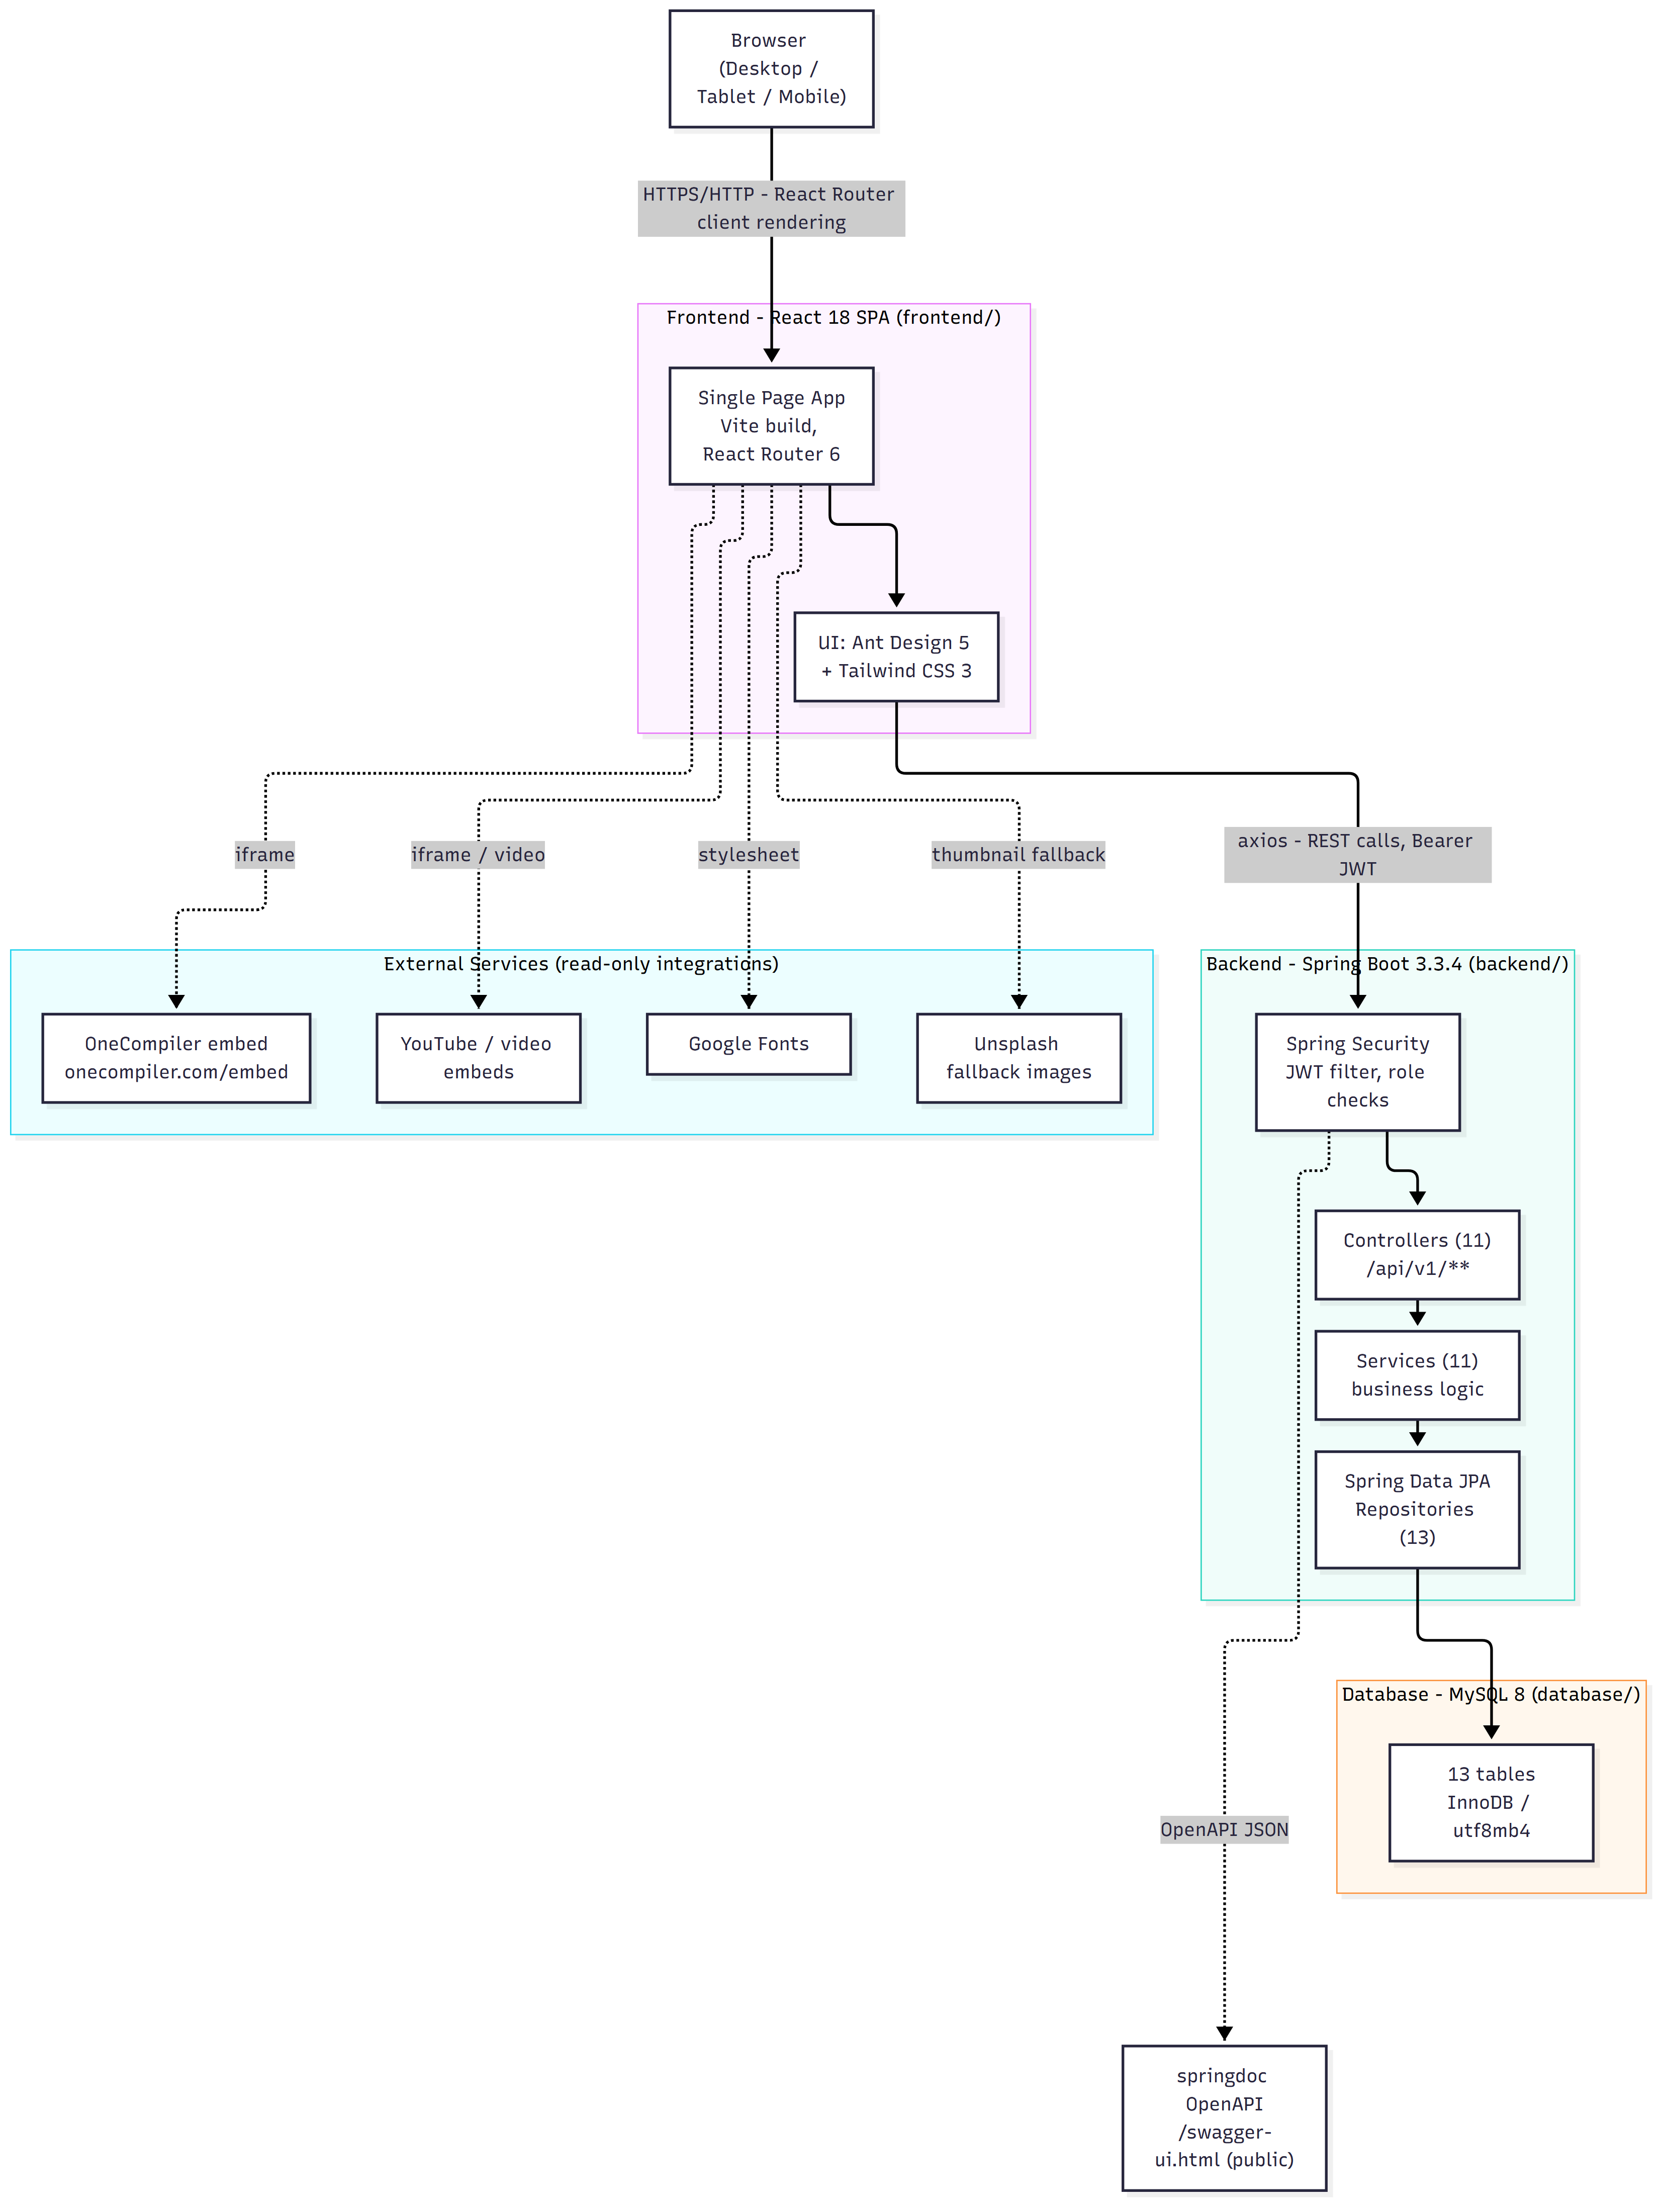
\includegraphics[width=0.9\textwidth]{diagrams/system-architecture.png}
    \caption{System architecture -- runtime components and external dependencies}
    \label{fig:sysarch-full}
\end{figure}

\subsection{Runtime components}
\begin{table}[H]
\centering
\caption{Runtime components and responsibilities}
\label{tab:runtime-components}
\begin{tabular}{@{}L{3.6cm}L{5.4cm}L{5.2cm}@{}}
\toprule
\textbf{Component} & \textbf{Responsibility} & \textbf{Key evidence} \\
\midrule
Browser & Renders SPA, holds session in \code{localStorage} & \pathref{frontend/src/context/AuthContext.jsx} \\
Vite dev server (dev) & Serves module graph on :3000, proxies \code{/api} & \pathref{frontend/vite.config.js} \\
Static host (prod) & Serves built \code{dist/} bundle & \code{npm run build} script \\
Axios client & Adds Bearer token, unwraps envelopes, maps errors & \pathref{frontend/src/api/client.js} \\
Spring Security filter chain & JWT validation, role enforcement, CORS & \pathref{backend/src/main/java/com/example/lms/config/SecurityConfig.java} \\
REST controllers (11) & HTTP binding + validation & \pathref{backend/src/main/java/com/example/lms/controller/} \\
Services (11) & Business rules, transactions & \pathref{backend/src/main/java/com/example/lms/service/} \\
JPA repositories (13) & Persistence & \pathref{backend/src/main/java/com/example/lms/repository/} \\
MySQL & Durable storage, constraints, indexes & \pathref{database/schema.sql} \\
springdoc & OpenAPI JSON + Swagger UI & \pathref{backend/src/main/java/com/example/lms/config/OpenApiConfig.java} \\
\bottomrule
\end{tabular}
\end{table}

\subsection{Trust boundaries}
\status{IMPLEMENTED (design) / PARTIAL (enforcement)}

\begin{enumerate}
    \item \textbf{Browser $\leftrightarrow$ API:} the only trusted client boundary. Tokens are issued and validated here; everything crossing this boundary is untrusted input validated by Bean Validation.
    \item \textbf{API $\leftrightarrow$ Database:} credentials via environment (\code{DB_URL} etc.); application connects as configured datasource user.
    \item \textbf{Client-side state:} \code{localStorage} tokens are convenience state, not a security boundary -- contract section 13 explicitly states frontend guards are not security controls.
    \item \textbf{Third-party origins:} OneCompiler iframe, YouTube, Google Fonts, Unsplash are outside the trust boundary and receive no user secrets.
\end{enumerate}

\subsection{Deployment view}
\status{PARTIAL}

The only artefact is \pathref{backend/Dockerfile} (multi-stage: JDK 21 alpine build with Maven, then JRE 21 alpine runtime, \code{EXPOSE 8080}). The frontend has no Dockerfile; no compose file ties components together; no production topology is defined. The verified development topology is: MySQL on \code{localhost:3306} + \code{./mvnw spring-boot:run} on :8080 + Vite on :3000. See Section~\ref{sec:deployment}.

\subsection{Architecture decisions (observed)}
\status{INFERRED (decisions are implicit in code)}

\begin{itemize}
    \item \textbf{Stateless JWT over server sessions} -- enables stateless scaling but forfeits revocation (see Section~\ref{sec:authentication}).
    \item \textbf{Monolith over microservices} -- one deployable JAR; appropriate for current scale; contract forbids unagreed technology changes.
    \item \textbf{Server-authoritative scoring} -- correctness and certificates decided in the backend; client is display-only.
    \item \textbf{Hibernate \code{ddl-auto: update}} over versioned migrations -- fast iteration, but schema history is not tracked (risk recorded in Section~\ref{sec:technical-debt}).
    \item \textbf{Static practice dataset} -- practice features shipped without backend work by explicit, documented design.
\end{itemize}

\section{Software Architecture}
\label{sec:software-architecture}

\subsection{Module map}
\status{IMPLEMENTED}

\begin{figure}[H]
    \centering
    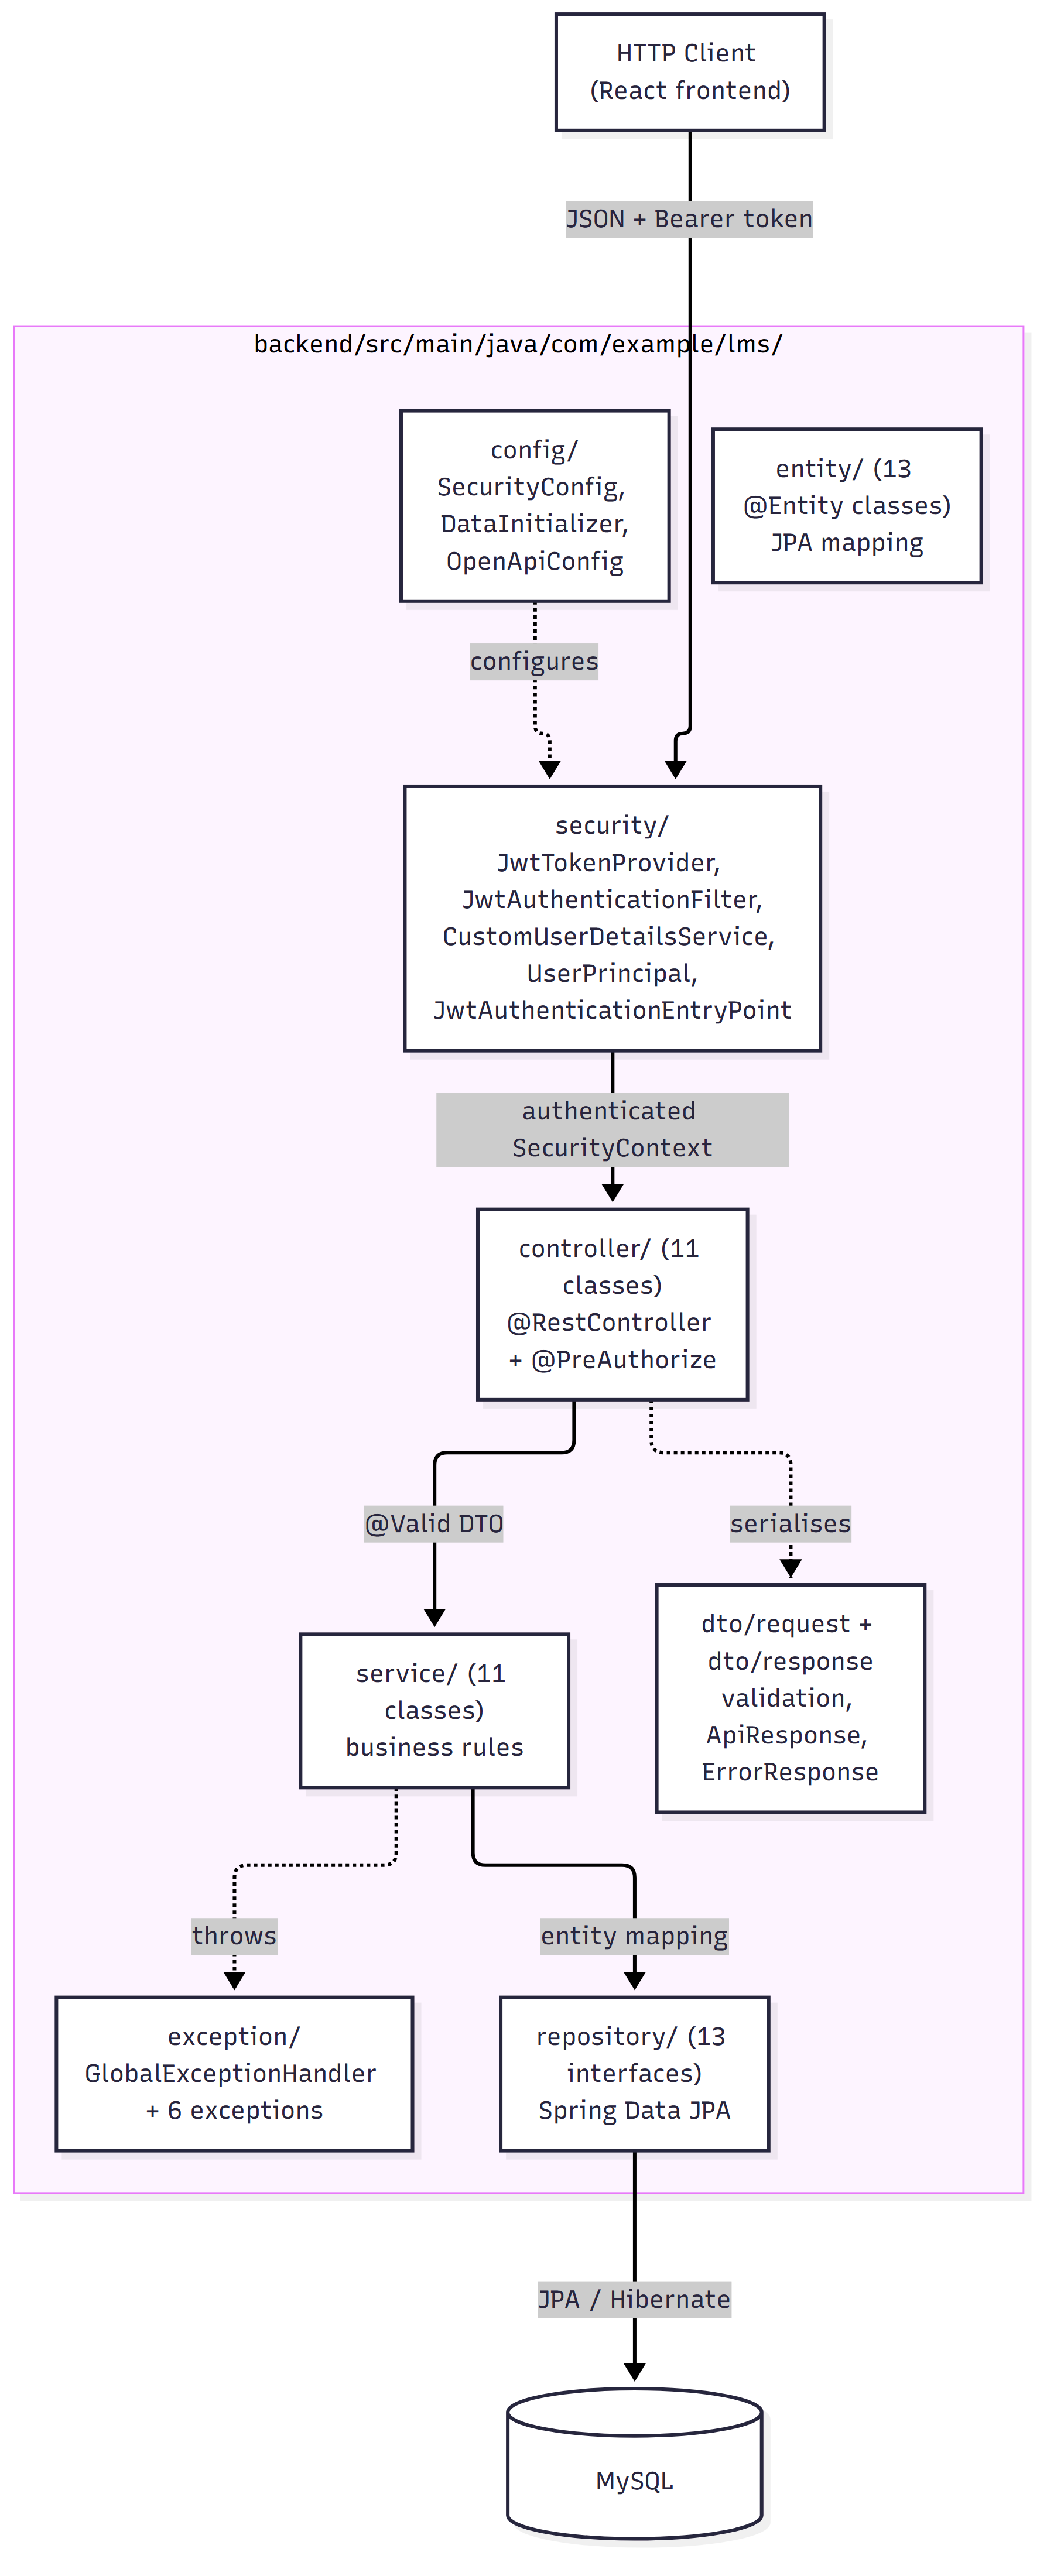
\includegraphics[width=0.92\textwidth]{diagrams/backend-layers.png}
    \caption{Backend software modules and their dependency direction}
    \label{fig:backend-layers}
\end{figure}

\begin{table}[H]
\centering
\caption{Software modules and ownership boundaries}
\label{tab:module-map}
\begin{tabular}{@{}L{4.0cm}L{5.6cm}L{4.6cm}@{}}
\toprule
\textbf{Module} & \textbf{Contents} & \textbf{Boundary rule} \\
\midrule
Frontend application & \pathref{frontend/src/} (api, components, pages, routes, context, hooks, data, utils) & Must not modify \pathref{backend/**} or \pathref{database/**} \\
Backend application & \pathref{backend/src/main/java/com/example/lms/} (8 packages) & Must not modify \pathref{frontend/**} \\
Database & \pathref{database/*.sql} & Owned exclusively by the backend workstream \\
API contract & DTO classes + \pathref{CONTRACT.md} sections 10--12 & Changes require cross-workstream agreement \\
Test suites & \pathref{backend/src/test/}, \pathref{frontend/src/test/} & Feature is incomplete until both suites pass \\
\bottomrule
\end{tabular}
\end{table}

\subsection{Backend packages (software units)}
\status{IMPLEMENTED}

\begin{table}[H]
\centering
\caption{Backend package responsibilities}
\label{tab:backend-packages}
\begin{tabular}{@{}L{2.9cm}L{6.6cm}L{4.7cm}@{}}
\toprule
\textbf{Package} & \textbf{Responsibility} & \textbf{Key classes} \\
\midrule
\code{config} & Framework wiring & SecurityConfig, DataInitializer, OpenApiConfig \\
\code{security} & Authentication pipeline & JwtTokenProvider, JwtAuthenticationFilter, CustomUserDetailsService, UserPrincipal, JwtAuthenticationEntryPoint \\
\code{controller} & HTTP adapters (11) & AuthController, CourseController, QuizController\dots \\
\code{dto} & API contracts (22 classes) & request/* + response/* \\
\code{service} & Business logic (11) & CourseService, QuizService, CertificateService\dots \\
\code{repository} & Persistence (13 interfaces) & Spring Data CRUD + derived queries \\
\code{entity} & Domain model (13) & User, Course, Lesson, Quiz, Certificate\dots \\
\code{exception} & Error taxonomy & GlobalExceptionHandler + 6 exceptions \\
\bottomrule
\end{tabular}
\end{table}

\subsection{Frontend software units}
\status{IMPLEMENTED}

\begin{table}[H]
\centering
\caption{Frontend module responsibilities}
\label{tab:frontend-modules}
\begin{tabular}{@{}L{3.2cm}L{7.0cm}L{4.0cm}@{}}
\toprule
\textbf{Module} & \textbf{Responsibility} & \textbf{Files} \\
\midrule
Entry & Bootstrap, antd theme, providers & \pathref{src/main.jsx}, \pathref{src/App.jsx} \\
Shell & Navbar, role sidebar/drawer, footer & AppShell, Navbar, Sidebar, Footer \\
Routing & Route tree + guards & \pathref{src/routes/} (AppRoutes, ProtectedRoute) \\
Pages & Screen-level composition (11 + 2 practice) & \pathref{src/pages/} \\
Components & Reusable UI (40+) & \pathref{src/components/} incl. practice/ and ui/ \\
API layer & 11 feature modules + shared client & \pathref{src/api/} \\
Auth state & Session context, role derivation & \pathref{src/context/AuthContext.jsx} \\
Practice data & Static problem dataset (swap boundary) & \pathref{src/data/practiceData.js} \\
Utilities & Constants, formatters & \pathref{src/utils/} \\
Tests & Vitest suites (8 files) & \pathref{src/test/} \\
\bottomrule
\end{tabular}
\end{table}

\subsection{Component interaction}
\status{IMPLEMENTED}

\begin{figure}[H]
    \centering
    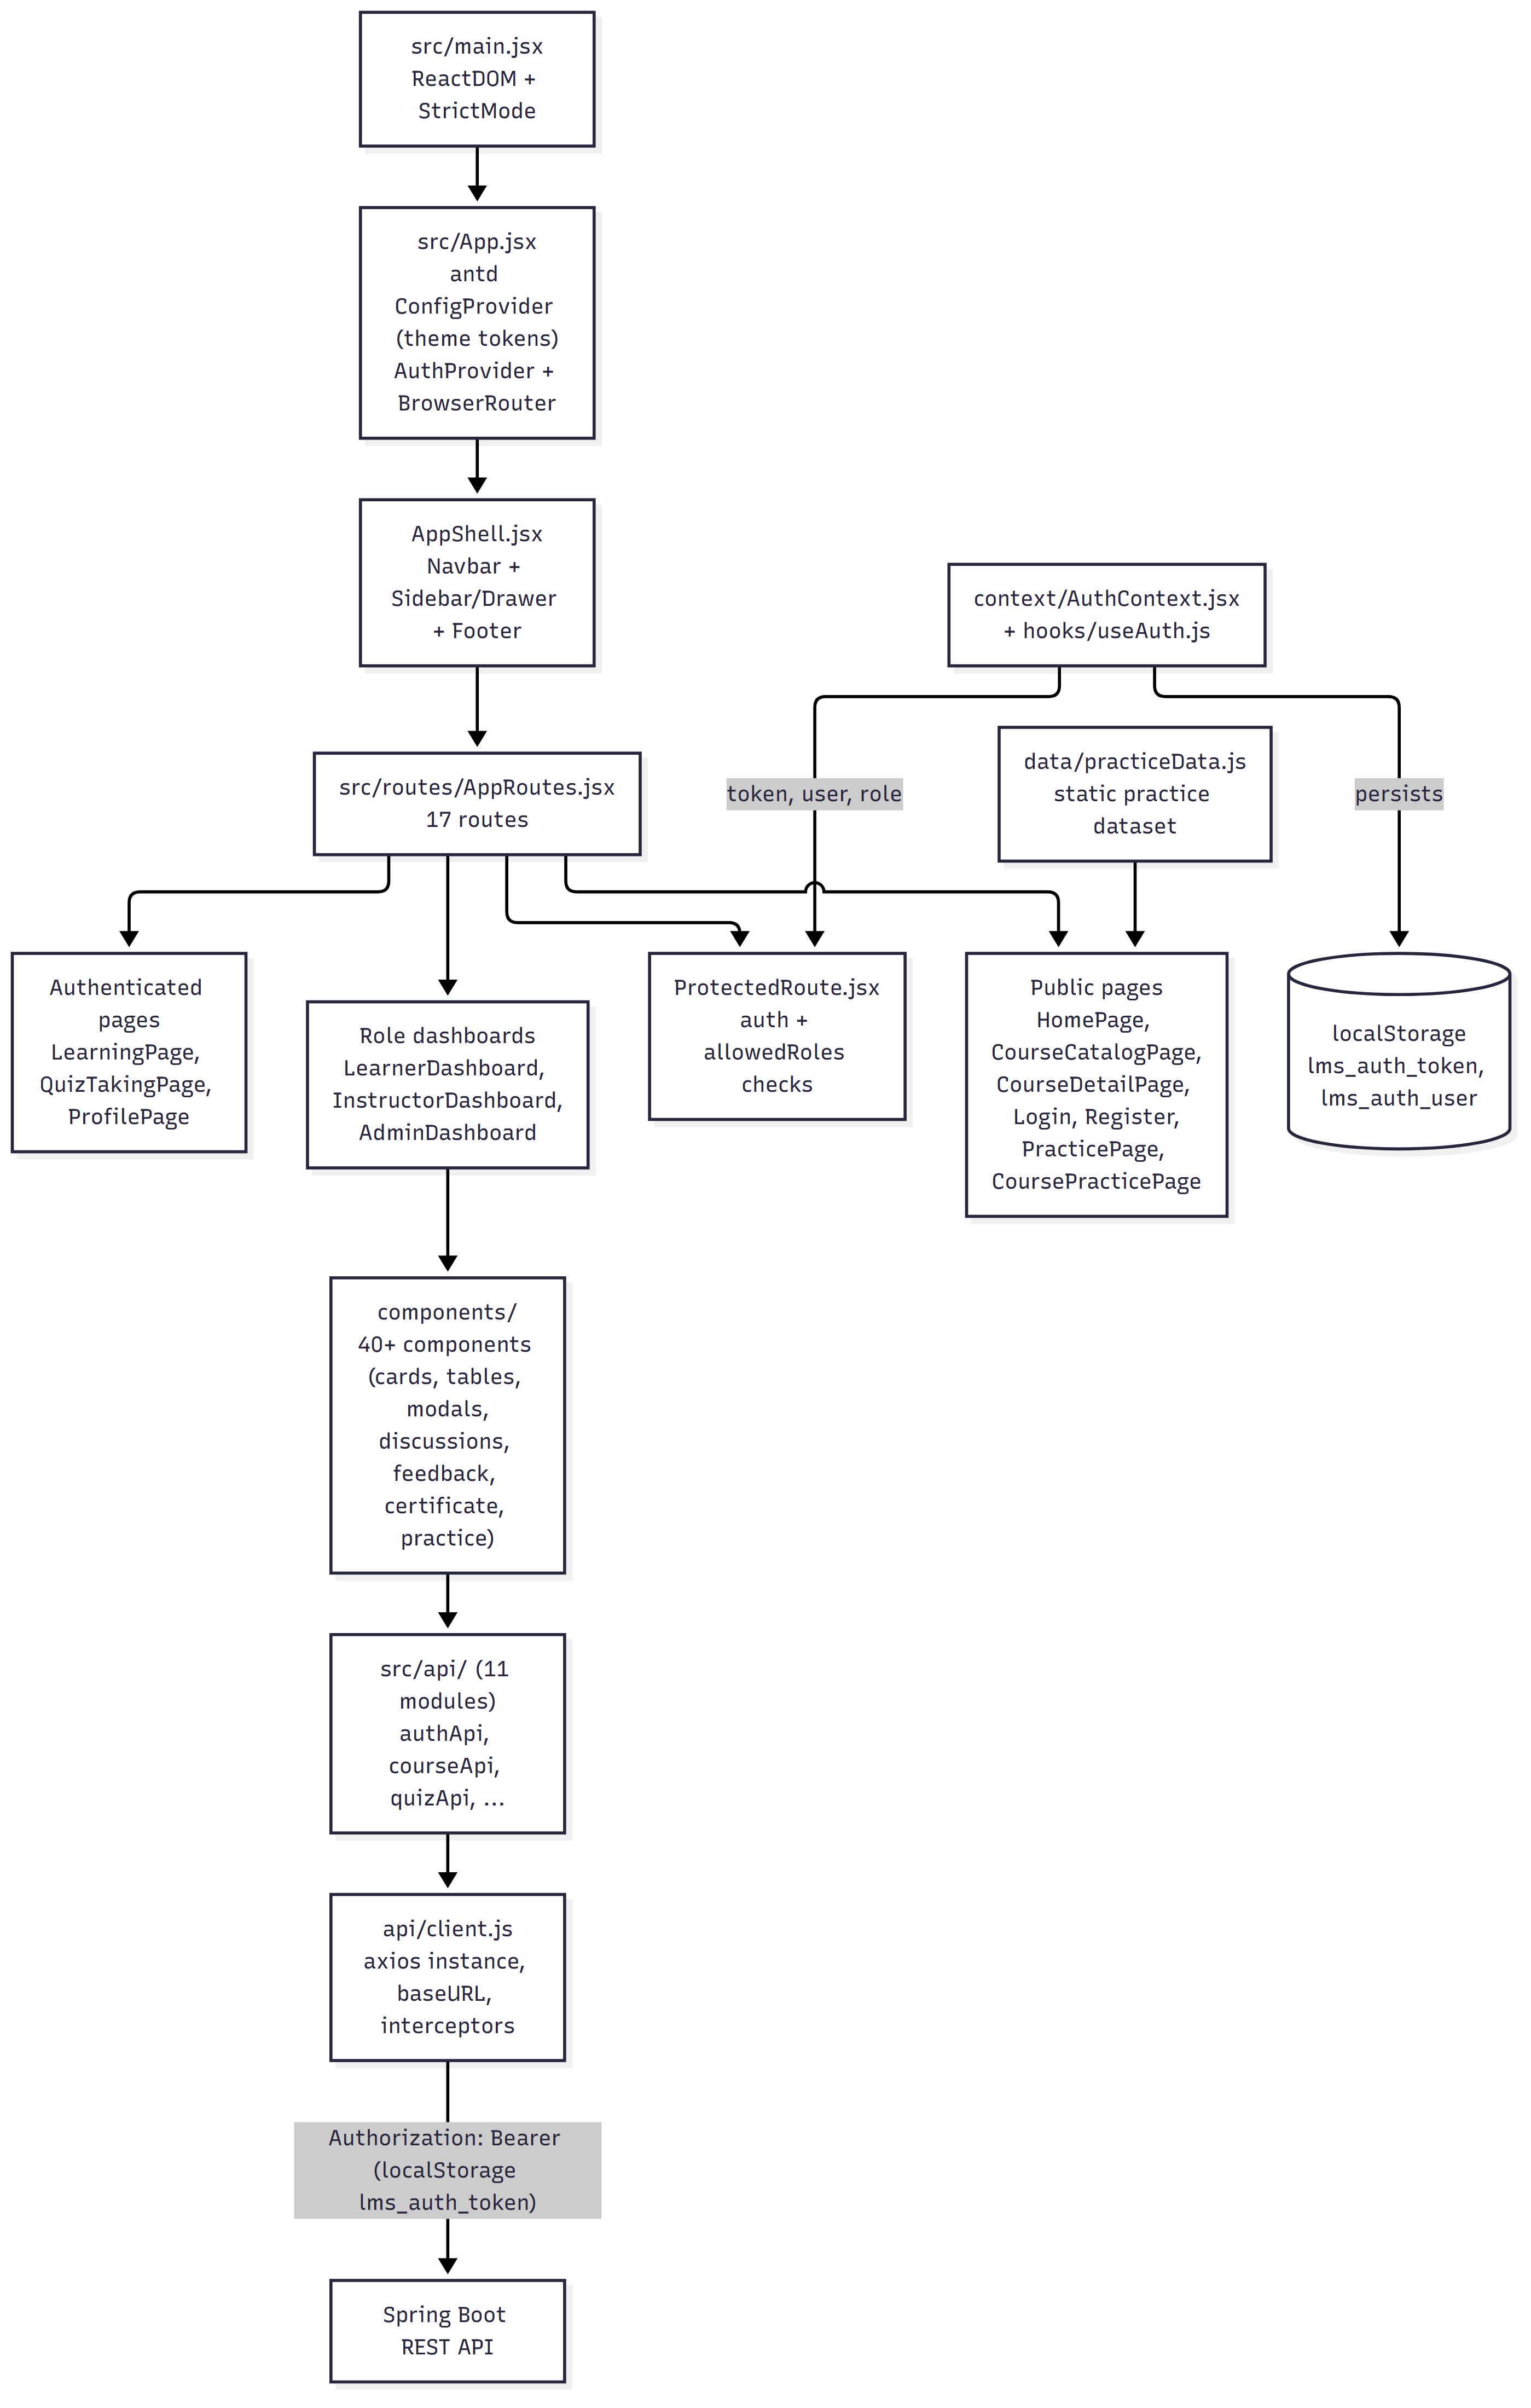
\includegraphics[width=0.95\textwidth]{diagrams/frontend-architecture.png}
    \caption{Frontend component architecture and data flow to the API}
    \label{fig:frontend-arch}
\end{figure}

\subsection{Data ownership and consistency}
\status{IMPLEMENTED}

\begin{itemize}
    \item MySQL is the single source of truth for users, catalogue, enrolments, progress, attempts, discussions, feedback and certificates.
    \item The backend owns all writes; the client may only send intentions (e.g.\ \code{{completed: true}}), never authoritative results (scores, eligibility).
    \item Transactions: service methods are \code{@Transactional} where multi-write (e.g.\ \code{AuthService.register}); each HTTP request is a single logical unit of work.
    \item Optimistic concurrency control (version columns) is \status{NOT IMPLEMENTED} -- concurrent updates last-write-wins.
\end{itemize}

\subsection{Cross-cutting concerns}
\begin{table}[H]
\centering
\caption{Cross-cutting concerns and their implementation points}
\label{tab:crosscutting}
\begin{tabular}{@{}L{3.4cm}L{6.2cm}L{4.6cm}@{}}
\toprule
\textbf{Concern} & \textbf{Mechanism} & \textbf{Location} \\
\midrule
Authentication & JWT filter before \code{UsernamePasswordAuthenticationFilter} & \pathref{security/JwtAuthenticationFilter.java} \\
Authorisation & URL rules + \code{@PreAuthorize} + service ownership checks & SecurityConfig, controllers, services \\
Validation & Bean Validation on DTOs & \code{dto/request/*} \\
Error handling & \code{@RestControllerAdvice} mapping to envelopes & \pathref{exception/GlobalExceptionHandler.java} \\
Logging & SLF4J with package log levels & \code{application.yml} \\
API docs & springdoc annotation-driven OpenAPI & \pathref{config/OpenApiConfig.java} \\
Client errors & Axios interceptor maps backend error codes & \pathref{frontend/src/api/client.js} \\
UI states & Loading/Error/Empty primitives & \pathref{frontend/src/components/common/} \\
\bottomrule
\end{tabular}
\end{table}

\section{High-Level Design}
\label{sec:high-level-design}

\subsection{Design scope}
\status{IMPLEMENTED}

High-level design covers the major runtime services and how they communicate. The system has exactly three internal services (frontend, backend, database) communicating synchronously over HTTP/JDBC -- there is no asynchronous messaging, no event bus and no scheduled processing in the repository.

\subsection{Service inventory and communication}
\begin{table}[H]
\centering
\caption{Major services and communication channels}
\label{tab:hld-services}
\begin{tabular}{@{}L{3.4cm}L{4.4cm}L{6.4cm}@{}}
\toprule
\textbf{Service} & \textbf{Communication} & \textbf{Contract} \\
\midrule
Frontend $\rightarrow$ Backend & HTTPS/HTTP JSON over REST (Axios) & \code{/api/v1/...}, Bearer JWT, \texttt{\{success, message, data\}} envelope \\
Backend $\rightarrow$ Frontend & JSON responses / error envelopes & \texttt{\{error: \{code, message, details?\}\}} \\
Backend $\rightarrow$ Database & JDBC via JPA/Hibernate & 13 tables, FK constraints, indexed lookups \\
Frontend $\rightarrow$ OneCompiler & \code{iframe} + \code{postMessage} & embed URL \code{https://onecompiler.com/embed/...}; message \code{eventType: populateCode} \\
Frontend $\rightarrow$ Media/CDN & \code{iframe}/\code{<video>}/\code{<img>} & YouTube embed URLs, Unsplash images, Google Fonts \\
Client $\rightarrow$ OpenAPI & GET \code{/v3/api-docs}, \code{/swagger-ui.html} & OpenAPI 3 (publicly readable) \\
\bottomrule
\end{tabular}
\end{table}

\subsection{Primary control flows}
\status{IMPLEMENTED}

\begin{figure}[H]
    \centering
    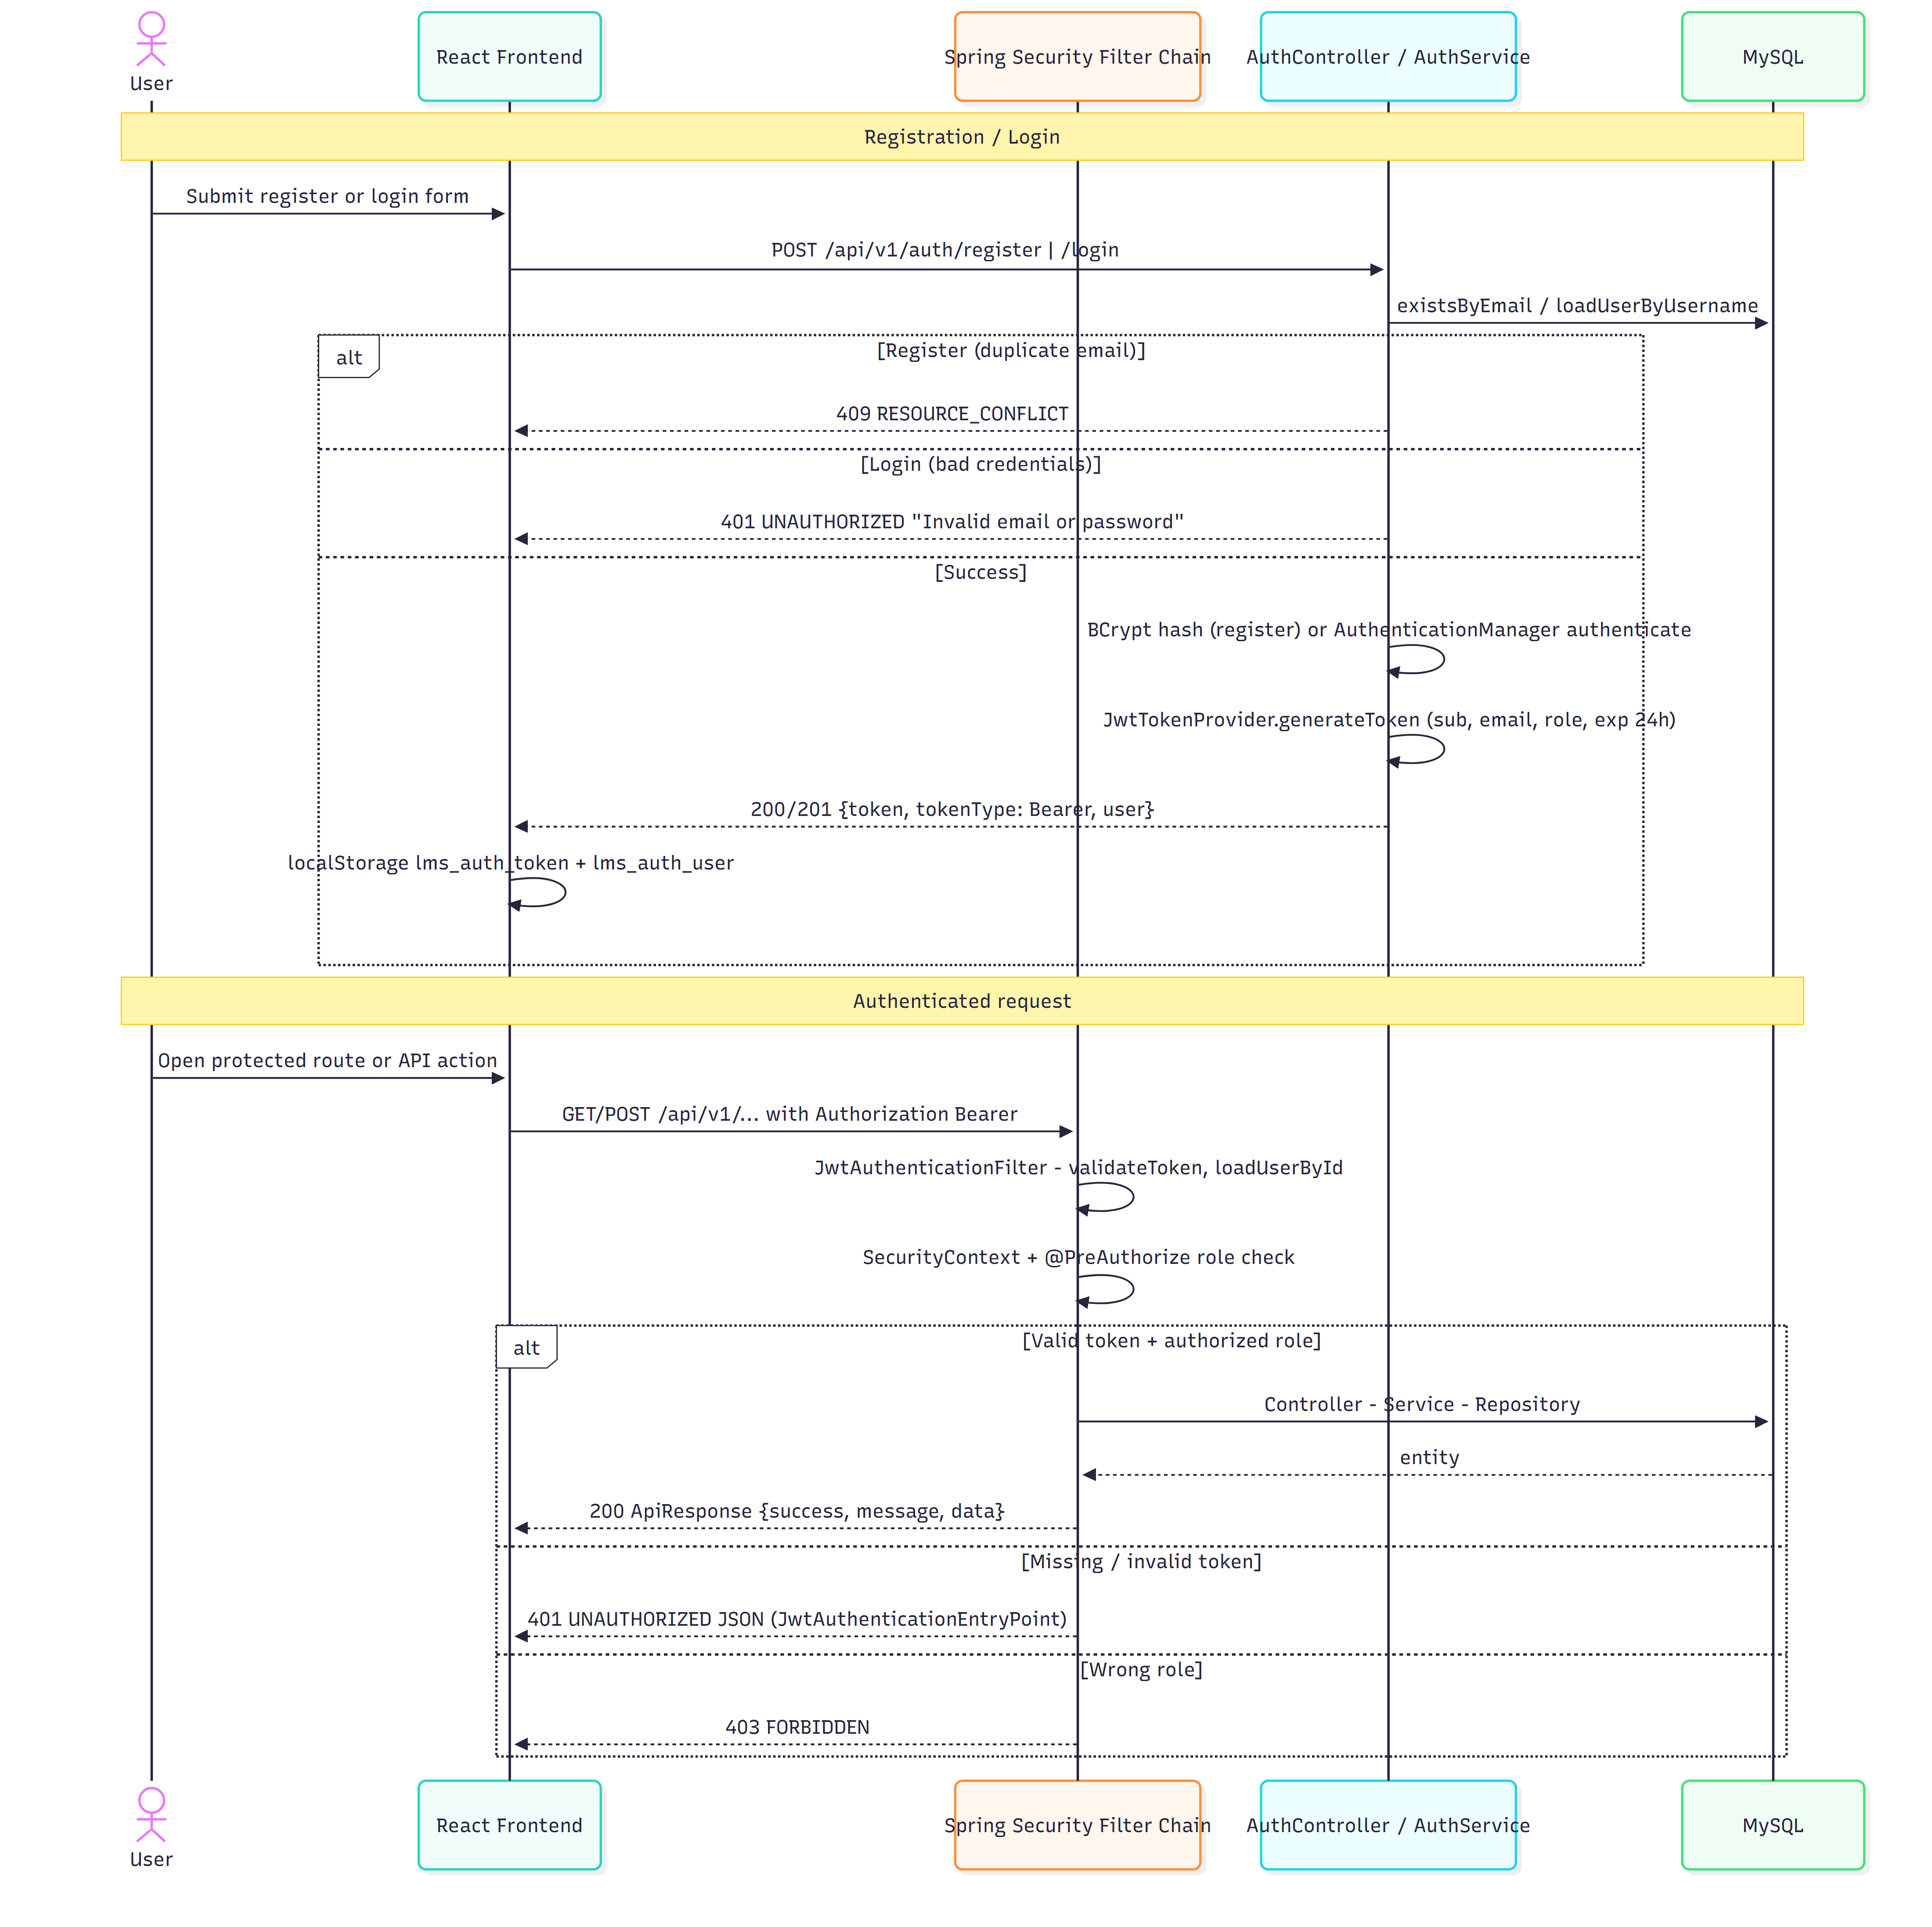
\includegraphics[width=0.95\textwidth]{diagrams/authentication-flow.png}
    \caption{Authentication and authorisation control flow}
    \label{fig:auth-flow}
\end{figure}

\begin{figure}[H]
    \centering
    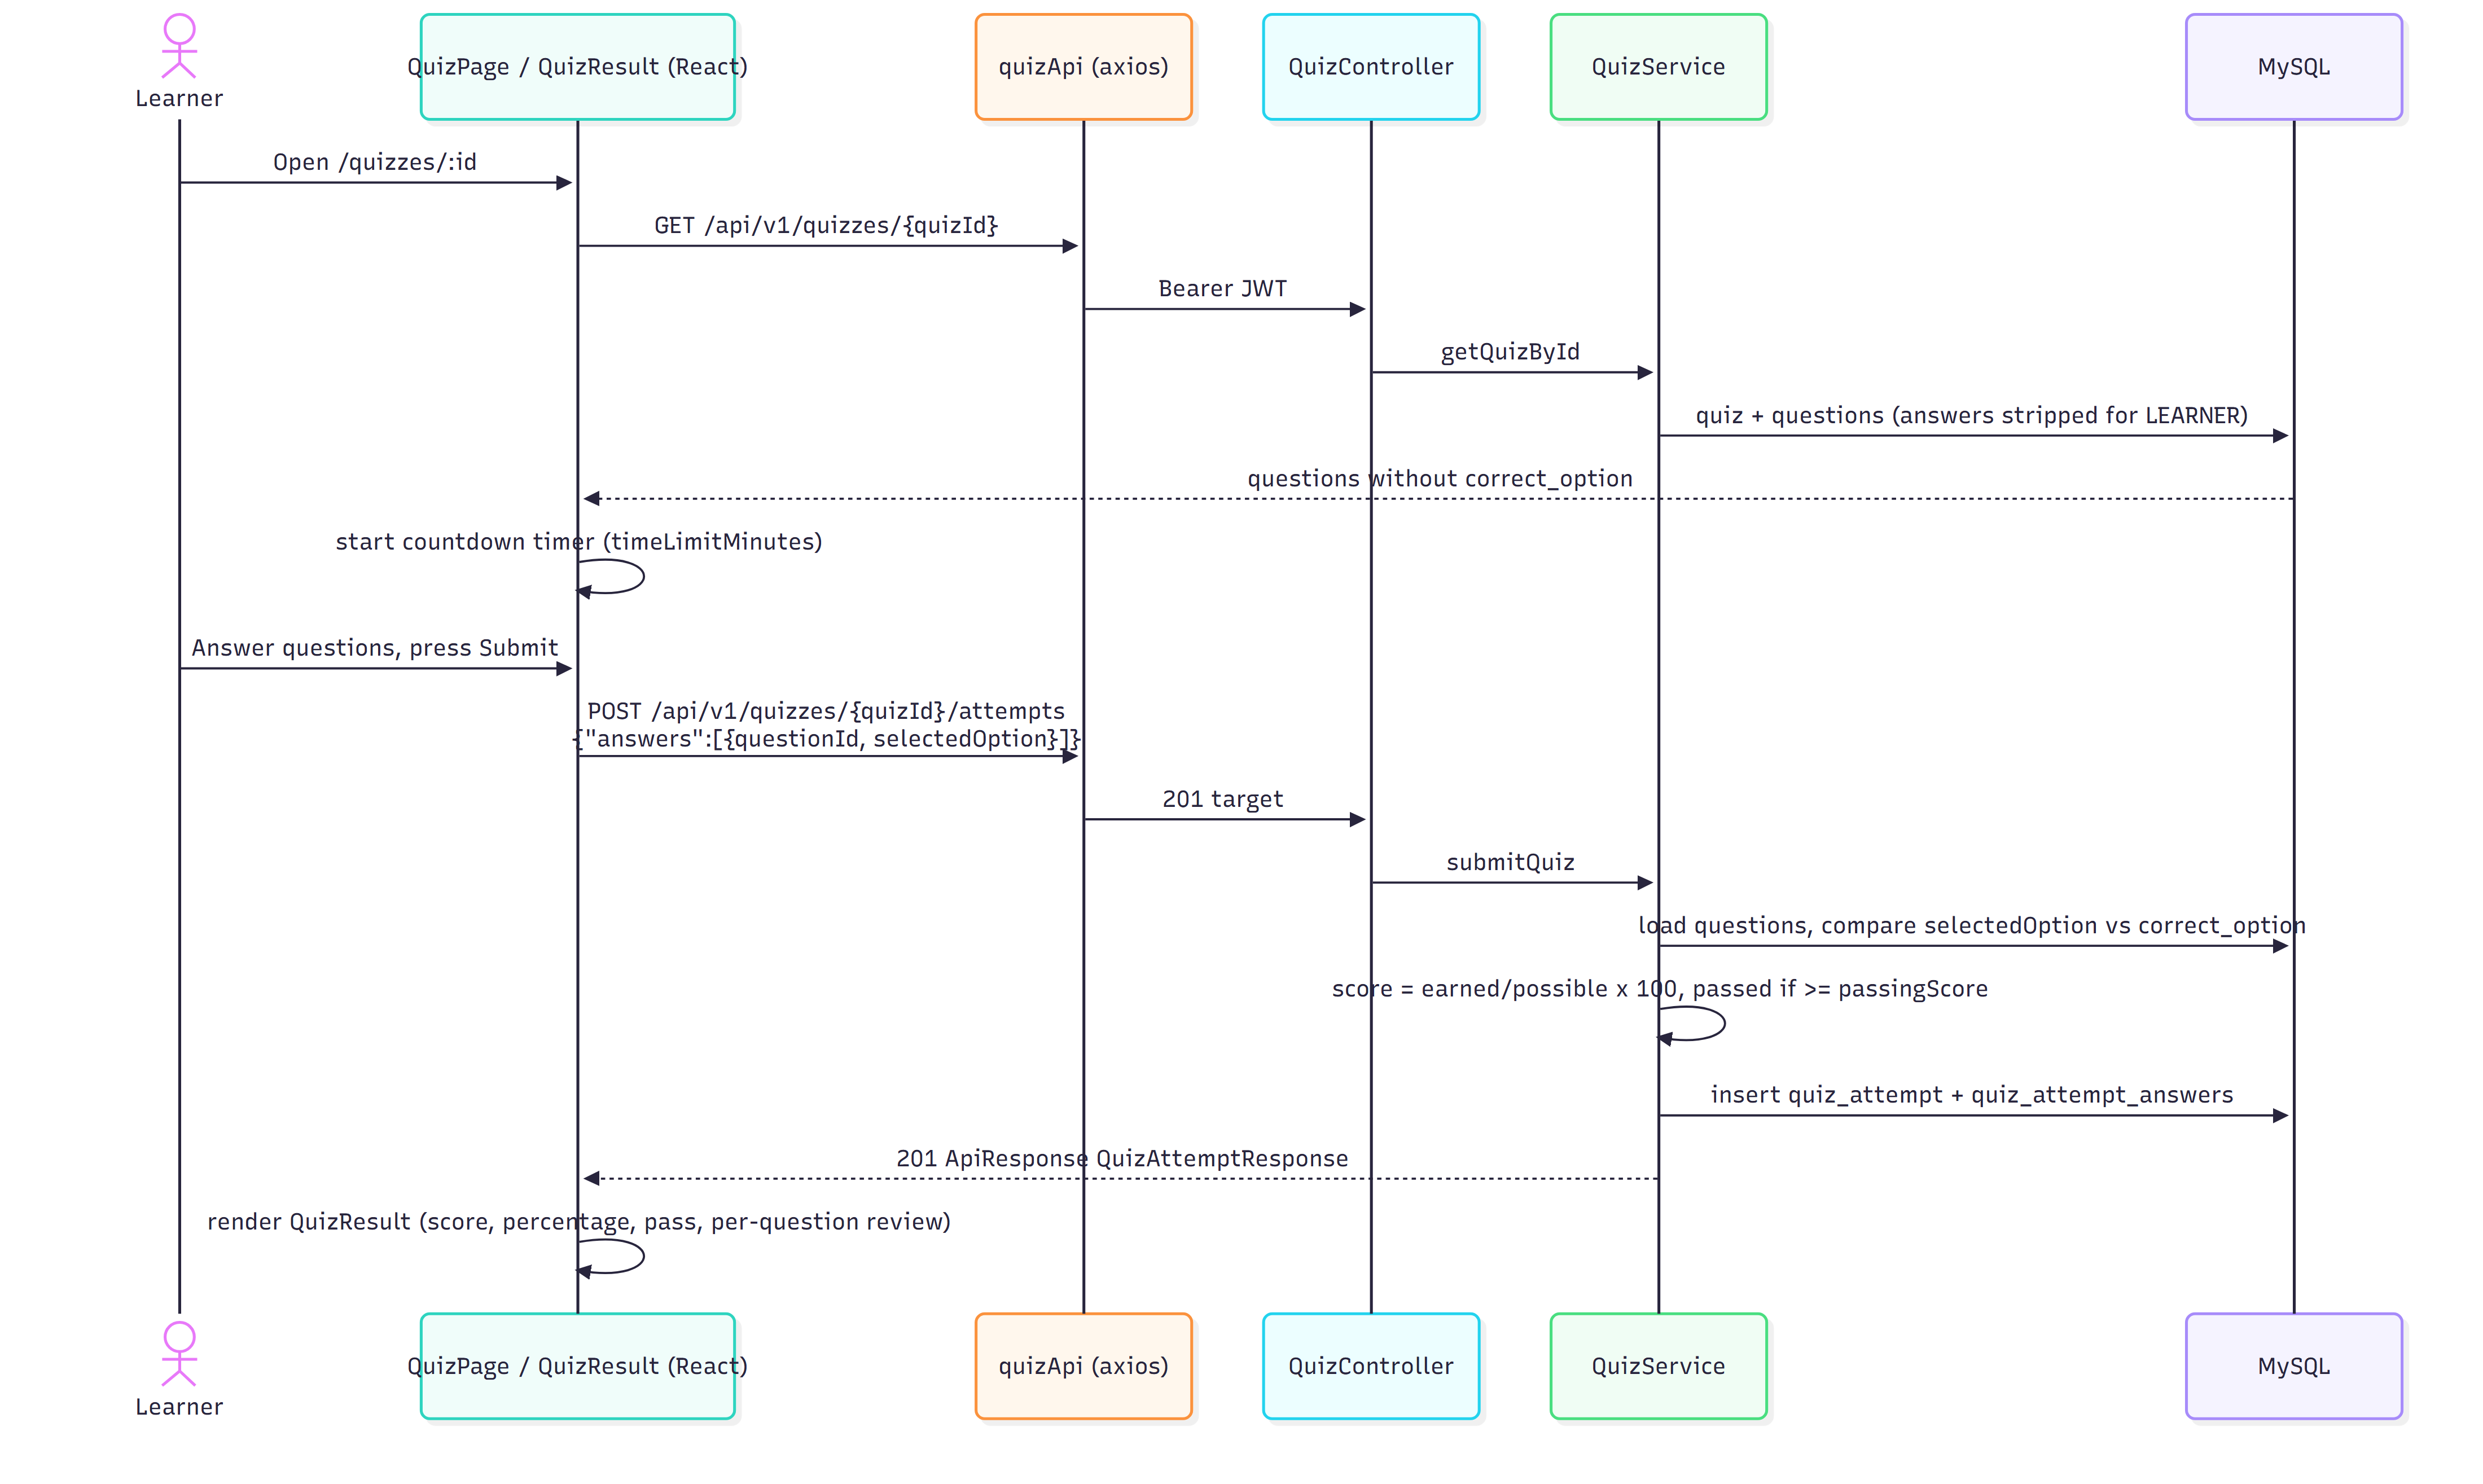
\includegraphics[width=0.95\textwidth]{diagrams/quiz-submission-sequence.png}
    \caption{Quiz submission sequence -- server-side authoritative scoring}
    \label{fig:quiz-sequence}
\end{figure}

\subsection{API surface overview}
\status{IMPLEMENTED}

47 mapped endpoints across 11 controllers (detail in Section~\ref{sec:api-documentation}):

\begin{table}[H]
\centering
\caption{API surface by domain}
\label{tab:api-surface}
\begin{tabular}{@{}L{4.6cm}C{2.0cm}C{2.4cm}L{4.2cm}@{}}
\toprule
\textbf{Domain} & \textbf{Endpoints} & \textbf{Base path} & \textbf{Public access?} \\
\midrule
Authentication & 3 & \code{/api/v1/auth} & Yes (register, login, logout) \\
Users & 3 & \code{/api/v1/users} & No (list is ADMIN-only) \\
Courses & 5 & \code{/api/v1/courses} & GET only \\
Categories & 5 & \code{/api/v1/categories} & GET only; writes ADMIN-only \\
Lessons & 5 & \code{/api/v1} & No \\
Enrollment & 3 & \code{/api/v1} & No \\
Progress & 3 & \code{/api/v1} & No \\
Quizzes \& attempts & 7 & \code{/api/v1} & No \\
Discussions & 4 & \code{/api/v1} & No \\
Feedback & 3 & \code{/api/v1} & No \\
Certificates & 2 & \code{/api/v1} & No \\
\bottomrule
\end{tabular}
\end{table}

\subsection{Data contracts}
\status{IMPLEMENTED}

\begin{lstlisting}[language=json,caption={Standard success and error envelopes (ApiResponse.java, ErrorResponse.java)}]
{"success": true, "message": "Login successful",
 "data": {"token": "eyJhbGciOi...", "tokenType": "Bearer",
          "user": {"id": 1, "email": "learner@example.com", "role": "LEARNER"}}}

{"error": {"code": "VALIDATION_ERROR",
           "message": "Validation failed for one or more fields",
           "details": ["email: must be a well-formed email address"]}}
\end{lstlisting}

\subsection{State management design}
\status{IMPLEMENTED}

\begin{itemize}
    \item \textbf{Server state} lives in MySQL; the client refetches after mutations (no global client cache such as React Query).
    \item \textbf{Session state} is two \code{localStorage} keys (\code{lms_auth_token}, \code{lms_auth_user}) mirrored into React context on mount.
    \item \textbf{URL state} encodes classroom and workspace context (\code{?lesson=}, \code{?problem=}, \code{?redirect=}).
    \item \textbf{Component state} (loading/error/data) is local to pages; no Redux/Zustand store exists.
\end{itemize}

\subsection{Error handling design}
\status{IMPLEMENTED}

\begin{enumerate}
    \item Backend: controller/service throws typed exceptions $\rightarrow$ \code{GlobalExceptionHandler} maps to status + code + message (+ field details for validation).
    \item Transport: Axios response interceptor normalises errors into \code{enhancedError} with \code{code}, \code{status}, \code{details}; network failures map to \code{NETWORK_ERROR}; timeouts use the 15\,000 ms limit.
    \item UI: \code{ErrorState} renders title/message/retry; per-action failures surface as antd \code{message.error} toasts.
\end{enumerate}

\noindent \textbf{Known gap:} HTTP 401 responses do not clear the stored session or redirect to login (\pathref{frontend/src/api/client.js}) -- logged out users with stale tokens see repeated failures until they log out manually. \status{IMPLEMENTED (defect)}

\section{Low-Level Design}
\label{sec:low-level-design}

Low-level design documents the principal classes and components, their responsibilities, state, data access and dependencies. Symbols are cited exactly as they appear in source.

\subsection{Backend -- service layer detail}
\status{IMPLEMENTED}

\begin{table}[H]
\centering
\caption{Service classes, responsibilities and key methods}
\label{tab:lld-services}
\begin{tabular}{@{}L{3.0cm}L{5.4cm}L{5.8cm}@{}}
\toprule
\textbf{Service} & \textbf{Responsibility} & \textbf{Key methods / rules} \\
\midrule
\code{AuthService} & Registration, login & \code{register} (409 on duplicate email, BCrypt, issues JWT, honours requested role); \code{login} (AuthenticationManager, 401 on bad credentials) \\
\code{UserService} & Profile read/update & \code{updateUser} (self or ADMIN; role change only by ADMIN); \code{getUserById} contains a no-op learner guard (defect) \\
\code{CourseService} & Catalogue CRUD & \code{getAllCourses} (Specification: search/category/status/instructor); \code{validateCourseOwnership} (admin or owning instructor); computed \code{totalLessons}, \code{totalEnrolled} \\
\code{CategoryService} & Category CRUD & Duplicate-name conflict check (case-insensitive) \\
\code{LessonService} & Lesson CRUD & Ownership via CourseService; default \code{orderIndex} = count+1; merges per-user completion flag \\
\code{EnrollmentService} & Enrol/drop/list & Duplicate \code{ENROLLED} $\rightarrow$ 409; re-enrol resets COMPLETED/DROPPED; \code{unenroll} sets DROPPED; self-or-ADMIN listing \\
\code{ProgressService} & Progress tracking & Find-or-create per user+lesson; \code{completed} and \code{percentage} kept consistent (100\% $\Leftrightarrow$ completed); auto-completes enrolment at 100\% \\
\code{QuizService} & Quiz authoring \& scoring & \code{includeAnswers} only for INSTRUCTOR/ADMIN; \code{submitQuiz} scores \code{earned/possible}, pass $\geq$ passing score; results scoped by role/ownership \\
\code{DiscussionService} & Threads \& replies & Top-level listing (\code{parentIsNull}); delete restricted to author/ADMIN; no enrolment gate \\
\code{FeedbackService} & Ratings & Enrolment required; one row per user+course (409 otherwise); edit restricted to author/ADMIN \\
\code{CertificateService} & Credential issuance & Eligibility: enrolled + all lessons complete + every quiz passed; idempotent; sets enrolment COMPLETED; code \code{LMS-xxxxxxxx-NNNN}; grade hard-coded DISTINCTION \\
\bottomrule
\end{tabular}
\end{table}

\subsection{Backend -- representative method detail}
\status{IMPLEMENTED}

\begin{lstlisting}[language=Java,caption={Ownership check used by course/lesson/quiz mutations (CourseService.validateCourseOwnership)}]
private void validateCourseOwnership(Course course, UserPrincipal currentUser) {
    if (currentUser.getRole() == User.Role.ADMIN) return;
    boolean owner = currentUser.getRole() == User.Role.INSTRUCTOR
            && course.getInstructor().getId().equals(currentUser.getId());
    if (!owner) throw new ForbiddenException(
            "You do not have permission to modify this course");
}
\end{lstlisting}

\begin{lstlisting}[language=Java,caption={Authoritative quiz scoring rule (QuizService.submitQuiz excerpt)}]
boolean isCorrect = question.getCorrectOption()
        .equalsIgnoreCase(submission.getSelectedOption().trim());
// earnedScore += points when correct; totalPossiblePoints over submitted answers
double scorePercentage = totalPossiblePoints > 0
        ? ((double) earnedScore / totalPossiblePoints) * 100.0 : 0.0;
boolean passed = scorePercentage >= quiz.getPassingScore(); // default 70
\end{lstlisting}

\noindent \textbf{Design note:} because \code{totalPossiblePoints} only accumulates points of questions present in the submission, unanswered questions do not reduce the percentage. \status{IMPLEMENTED (behaviour) -- see Section~\ref{sec:known-issues}}.

\subsection{Backend -- persistence access}
\status{IMPLEMENTED}

\begin{itemize}
    \item All 13 repositories extend \texttt{JpaRepository$<$Entity, Long$>$} with derived query methods (e.g.\ \code{findByEmail}, \code{existsByQuizIdAndUserIdAndPassedTrue}, \code{findByCourseIdAndParentIsNullOrderByCreatedAtDesc}).
    \item No native queries, no \code{JdbcTemplate}, no specification API except \code{CourseRepository.findAll(Specification)}.
    \item Fetch strategy: \code{@ManyToOne} default EAGER for user/course links used in responses, LAZY for lesson/course back-references; collections (\code{Quiz.questions}, \code{QuizAttempt.answers}, \code{Discussion.replies}) are LAZY with cascade ALL + orphanRemoval.
    \item Timestamps set by \code{@PrePersist}/\code{@PreUpdate} callbacks inside entities.
\end{itemize}

\subsection{Backend -- data initialisation logic}
\status{IMPLEMENTED}

\pathref{backend/src/main/java/com/example/lms/config/DataInitializer.java} runs on every startup:
\begin{enumerate}
    \item If \code{categoryRepository.count() == 0}: insert 4 categories (Web Development, Computer Science, Cloud \& DevOps, Data Science \& AI).
    \item If \code{userRepository.count() == 0}: insert 3 users with BCrypt-encoded \emph{hardcoded} passwords: \code{admin@example.com}/\code{admin123} (ADMIN), \code{instructor@example.com}/\code{password123} (INSTRUCTOR), \code{learner@example.com}/\code{password123} (LEARNER).
\end{enumerate}

\noindent There is no profile or property guard; the seed runs on any empty database, including production. \textbf{Finding S-02, Section~\ref{sec:security}}.

\subsection{Frontend -- state and data access detail}
\status{IMPLEMENTED}

\begin{table}[H]
\centering
\caption{Frontend state, storage and data access}
\label{tab:lld-frontend-state}
\begin{tabular}{@{}L{3.4cm}L{5.6cm}L{5.2cm}@{}}
\toprule
\textbf{Concern} & \textbf{Implementation} & \textbf{State/keys} \\
\midrule
Session & \pathref{frontend/src/context/AuthContext.jsx} & \code{lms_auth_token}, \code{lms_auth_user}; \code{isLoading} restore gate \\
Derived auth & \code{role}, \code{isAuthenticated}, \code{isLearner/isInstructor/isAdmin} & Computed on each context value build \\
Route guards & \pathref{frontend/src/routes/ProtectedRoute.jsx} & loading $\rightarrow$ spinner; unauth $\rightarrow$ \code{/login?redirect=}; wrong role $\rightarrow$ 403 card \\
HTTP & \pathref{frontend/src/api/client.js} & base URL \code{VITE_API_BASE_URL} or \code{http://localhost:8080}; 15 s timeout; Bearer injection; envelope unwrapping \\
Page data & Local \code{useState} + \code{useEffect} fetches & loading/error/data triples per page \\
URL query & \code{useSearchParams} & \code{lesson}, \code{problem}, \code{redirect} \\
\bottomrule
\end{tabular}
\end{table}

\subsection{Frontend -- key component behaviours}
\status{IMPLEMENTED}

\begin{table}[H]
\centering
\caption{Representative component logic}
\label{tab:lld-components}
\begin{tabular}{@{}L{3.4cm}L{9.8cm}@{}}
\toprule
\textbf{Component} & \textbf{Behaviour} \\
\midrule
\pathref{frontend/src/components/LessonPlayer.jsx} & Detects media type (YouTube/Vimeo/\code{.mp4} $\rightarrow$ embed; other URL $\rightarrow$ external-resource button; none $\rightarrow$ text lesson); \code{recordLessonProgress} posts \code{{completed: true, completionPercentage: 100, watchTimeSeconds}} \\
\pathref{frontend/src/components/QuizPage.jsx} & One-question-at-a-time with palette; countdown from \code{timeLimitMinutes}; confirmation modal on partial submit; delegates to \code{QuizResult} \\
\pathref{frontend/src/components/practice/OneCompilerEditor.jsx} & Builds embed URL (language slug + \code{listenToEvents}); injects starter code via \code{postMessage} on load, after 400 ms, and on button click \\
\pathref{frontend/src/components/EnrollmentButton.jsx} & Unauth $\rightarrow$ login redirect; instructor $\rightarrow$ blocked; enrolled $\rightarrow$ Continue Learning (+ optional Drop); else enrol via API \\
\pathref{frontend/src/components/CertificateCard.jsx} & Renders code/learner/course/grade/date; \code{window.print()} for PDF saving \\
\pathref{frontend/src/components/InstructorDashboard.jsx} & Client-side course scoping; tabs for Lessons/Assessments; modals for course/lesson/quiz authoring; submissions modal with pass/fail badges \\
\bottomrule
\end{tabular}
\end{table}

\subsection{Dependencies (internal)}
\status{IMPLEMENTED}

\begin{lstlisting}[language=bash,caption={Internal dependency direction (no cycles beyond declared parent-child)}]
Controller --> Service --> Repository --> Entity
Service   --> other Service (CourseService <-- Lesson/Quiz/Certificate/Enrollment)
Service   --> Security (UserPrincipal for identity/role)
Component --> api module --> client (axios) --> backend
Page      --> components --> api modules
Context   --> authApi ; Pages --> useAuth()
\end{lstlisting}

\section{Frontend Architecture}
\label{sec:frontend-architecture}

\subsection{Application entry and providers}
\status{IMPLEMENTED}

\begin{lstlisting}[language=bash,caption={Bootstrap chain (frontend/src/main.jsx, frontend/src/App.jsx)}]
main.jsx
  -> <StrictMode> -> <AuthProvider> -> <BrowserRouter> -> <ConfigProvider antdTheme>
       -> <AppShell> (Navbar + Sidebar/Drawer + main + Footer)
            -> <AppRoutes />
\end{lstlisting}

\noindent The antd theme in \pathref{frontend/src/App.jsx} injects the design tokens (black primary, 4px radius, 40px control height, custom component overrides) described in Section~\ref{sec:design-system}.

\subsection{Routing}
\status{IMPLEMENTED}

\pathref{frontend/src/routes/AppRoutes.jsx} declares 17 routes:

\begin{table}[H]
\centering
\caption{Frontend route table}
\label{tab:frontend-routes}
\begin{tabular}{@{}L{5.0cm}L{4.6cm}L{4.4cm}@{}}
\toprule
\textbf{Path} & \textbf{Component} & \textbf{Guard} \\
\midrule
\code{/} & HomePage & public \\
\code{/login} & LoginPage & public (\code{?redirect=} honoured) \\
\code{/register} & RegisterPage & public \\
\code{/courses} & CourseCatalogPage & public \\
\code{/courses/:id} & CourseDetailPage (CourseDetails) & public \\
\code{/practice} & PracticePage & public \\
\code{/courses/:courseId/practice} & CoursePracticePage & public \\
\code{/courses/:courseId/learn} & LearningPage & authenticated \\
\code{/quizzes/:id} & QuizTakingPage (QuizPage) & authenticated \\
\code{/learner}, \code{/learner/certificates} & LearnerDashboard & LEARNER, ADMIN \\
\code{/instructor}, \code{/instructor/courses/new} & InstructorDashboard & INSTRUCTOR, ADMIN \\
\code{/admin}, \code{/admin/users}, \code{/admin/categories} & AdminDashboard & ADMIN \\
\code{/profile} & ProfilePage & authenticated \\
\code{*} & NotFoundPage & -- \\
\bottomrule
\end{tabular}
\end{table}

\subsection{Guard semantics}
\status{IMPLEMENTED (with known gaps)}

\pathref{frontend/src/routes/ProtectedRoute.jsx}:
\begin{itemize}
    \item \code{isLoading} $\rightarrow$ full-page \code{LoadingState} (``Authenticating\dots'').
    \item Not authenticated $\rightarrow$ redirect to \code{/login?redirect=<path>} (the original query string is dropped -- defect KI-10).
    \item Authenticated but role not in \code{allowedRoles} $\rightarrow$ inline 403 card (``Access Restricted'') with a full-page-home button.
    \item Guards are usability controls only; the backend enforces authorisation (\pathref{CONTRACT.md} section 13).
\end{itemize}

\subsection{Navigation structure}
\status{IMPLEMENTED}

\begin{itemize}
    \item \textbf{Navbar} (sticky): brand images, ``Create Course'' link (INSTRUCTOR only), auth-aware dropdown (Dashboard, Profile, Log Out) with avatar and role badge.
    \item \textbf{Sidebar} (desktop, authenticated): role-specific \code{NavLink} sets -- ADMIN: \code{/admin}, \code{/courses}, \code{/admin/users}, \code{/admin/categories}, \code{/profile}; INSTRUCTOR: \code{/instructor}, \code{/courses}, \code{/instructor/courses/new}, \code{/profile}; LEARNER: \code{/learner}, \code{/courses}, \code{/learner/certificates}, \code{/profile}. Mobile uses an antd Drawer (width 320).
    \item \textbf{Footer}: five columns (brand, Learn, Profile, Account, Practice). Three links point to routes that do not exist (\code{/learner/enrollments}, \code{/learner/progress}, \code{/settings}) -- defect KI-01.
\end{itemize}

\subsection{API layer}
\status{IMPLEMENTED}

\begin{table}[H]
\centering
\caption{Frontend API modules and the endpoints they call}
\label{tab:frontend-api-modules}
\begin{tabular}{@{}L{3.0cm}L{10.4cm}@{}}
\toprule
\textbf{Module} & \textbf{Endpoints invoked} \\
\midrule
\code{authApi} & \code{POST /api/v1/auth/register}, \code{POST /api/v1/auth/login}, \code{POST /api/v1/auth/logout} \\
\code{userApi} & \code{GET /api/v1/users/{id}}, \code{PUT /api/v1/users/{id}}, \code{GET /api/v1/users} \\
\code{categoryApi} & \code{GET/POST/PUT/DELETE /api/v1/categories[...]}, \code{GET /api/v1/categories/{id}} \\
\code{courseApi} & \code{GET /api/v1/courses?search&categoryId&status&instructorId}, \code{GET/PUT/DELETE /api/v1/courses/{id}}, \code{POST /api/v1/courses} \\
\code{enrollmentApi} & \code{POST /api/v1/courses/{id}/enroll}, \code{DELETE .../enroll?userId=}, \code{GET /api/v1/users/{id}/enrollments} \\
\code{lessonApi} & \code{GET/POST /api/v1/courses/{id}/lessons}, \code{GET/PUT/DELETE /api/v1/lessons/{id}} \\
\code{progressApi} & \code{GET /api/v1/courses/{id}/progress}, \code{POST/PATCH /api/v1/lessons/{id}/progress} \\
\code{quizApi} & \code{GET /api/v1/courses/{id}/quizzes}, \code{GET/PUT/DELETE /api/v1/quizzes/{id}}, \code{POST .../attempts}, \code{GET .../results}, \code{POST /api/v1/courses/{id}/quizzes} \\
\code{discussionApi} & \code{GET/POST /api/v1/courses/{id}/discussions}, \code{POST /api/v1/discussions/{id}/replies}, \code{DELETE /api/v1/discussions/{id}} \\
\code{feedbackApi} & \code{GET/POST /api/v1/courses/{id}/feedback}, \code{PUT /api/v1/feedback/{id}} \\
\code{certificateApi} & \code{GET/POST /api/v1/courses/{id}/certificate} \\
\bottomrule
\end{tabular}
\end{table}

\noindent Every path above was cross-checked against the Spring controllers -- there are no phantom frontend calls. The shared \pathref{frontend/src/api/client.js} attaches the Bearer token, unwraps envelopes, and normalises errors (Section~\ref{sec:high-level-design}).

\subsection{Component inventory}
\status{IMPLEMENTED}

\begin{table}[H]
\centering
\caption{Component inventory (selected, with purpose)}
\label{tab:component-inventory}
\begin{tabular}{@{}L{3.6cm}L{9.6cm}@{}}
\toprule
\textbf{Component} & \textbf{Purpose} \\
\midrule
AppShell / Navbar / Sidebar / Footer & Application chrome and role-aware navigation \\
LearnerDashboard & KPI tiles, active/completed tabs, certificates list \\
InstructorDashboard & Course table, content manager tabs (Lessons, Assessments), authoring modals, submissions modal \\
AdminDashboard & KPI tiles, user directory, category CRUD, course moderation \\
CourseCard / CourseList / CourseDetails & Catalogue presentation and detail tabs (Syllabus, Assessments, Practice, Discussions, Reviews) \\
EnrollmentButton / ProgressBar & Enrolment interaction and progress display \\
LessonPlayer / LearningPage & Classroom: media player, curriculum sidebar, certificate modal \\
QuizPage / QuizResult / QuizCard & Timed assessment flow and review \\
DiscussionList / DiscussionItem & Threads with recursive replies (UI depth $\leq$ 2) \\
FeedbackForm & Ratings, average, star distribution, reviews \\
CertificateCard & Printable credential \\
practice/* & Problem list, workspace, statement panel, OneCompiler editor, course practice tab \\
common/* & LoadingState, ErrorState, EmptyState (tested state primitives) \\
ui/* & Card, GradientRibbon, SectionHeader, Badge, StatTile, WordmarkBanner (design-system kit) \\
\bottomrule
\end{tabular}
\end{table}

\subsection{Practice module structure}
\status{IMPLEMENTED}

\pathref{frontend/src/components/practice/} implements a self-contained feature: data access strictly through \code{fetchPracticeProblems} in \pathref{frontend/src/data/practiceData.js} (a local dataset of 7 problems across Python, JavaScript and Java, three of them bound to seeded course ids), rendering problem statements and a OneCompiler iframe. The file header documents the intended swap boundary: replace the local promise with \code{apiClient.get(...)} when a backend practice API exists. \status{IMPLEMENTED (client) / NOT IMPLEMENTED (server)}.

\subsection{Build pipeline}
\status{IMPLEMENTED}

\begin{lstlisting}[language=bash,caption={Verified frontend commands (frontend/package.json)}]
npm install
npm run dev        # vite, port 3000, /api proxy to :8080
npm run build      # vite build -> dist/
npm run preview    # vite preview
npm test           # vitest run (39 tests)
npm run test:watch # vitest watch
\end{lstlisting}

\noindent There is no lint or format script; no ESLint/Prettier configuration exists in the repository. \status{NOT IMPLEMENTED (linting)}

\section{Backend Architecture}
\label{sec:backend-architecture}

\subsection{Layered structure}
\status{IMPLEMENTED}

The backend follows the canonical layering mandated by \pathref{CONTRACT.md} section 7:

\begin{center}
\texttt{Controller $\rightarrow$ Service $\rightarrow$ Repository $\rightarrow$ Database}
\end{center}

\noindent Controllers never touch repositories directly (verified: all persistence calls go through service classes); DTOs isolate the wire format from JPA entities; security components sit \emph{beside} the layers in the servlet filter chain.

\subsection{Component inventory}
\begin{table}[H]
\centering
\caption{Backend component counts}
\label{tab:backend-inventory}
\begin{tabular}{@{}L{5.0cm}C{2.2cm}L{6.4cm}@{}}
\toprule
\textbf{Component type} & \textbf{Count} & \textbf{Location} \\
\midrule
REST controllers & 11 & \pathref{backend/src/main/java/com/example/lms/controller/} \\
Service classes & 11 & \pathref{backend/src/main/java/com/example/lms/service/} \\
JPA repositories & 13 & \pathref{backend/src/main/java/com/example/lms/repository/} \\
Entities & 13 & \pathref{backend/src/main/java/com/example/lms/entity/} \\
Request DTOs & 15 & \pathref{backend/src/main/java/com/example/lms/dto/request/} \\
Response DTOs & 15 & \pathref{backend/src/main/java/com/example/lms/dto/response/} \\
Security components & 5 & \pathref{backend/src/main/java/com/example/lms/security/} \\
Exception types & 7 (1 advice + 6) & \pathref{backend/src/main/java/com/example/lms/exception/} \\
Configuration classes & 3 & \pathref{backend/src/main/java/com/example/lms/config/} \\
\bottomrule
\end{tabular}
\end{table}

\subsection{Request lifecycle}
\status{IMPLEMENTED}

\begin{enumerate}
    \item \textbf{Container} receives HTTP request on port \code{PORT} (8080 default).
    \item \textbf{JwtAuthenticationFilter} (\code{OncePerRequestFilter}) extracts \code{Authorization: Bearer} token, validates signature/expiry, loads the user by id, and populates \code{SecurityContextHolder}. Failures are logged and the request continues unauthenticated.
    \item \textbf{Spring Security authorisation} applies URL matchers (\code{permitAll} / \code{hasRole}) or throws \code{AccessDeniedException}.
    \item \textbf{DispatcherServlet} routes to a controller method; \code{@Valid} triggers Bean Validation.
    \item \textbf{Method security} evaluates \code{@PreAuthorize} expressions (\code{hasRole('ADMIN')}, \code{hasAnyRole('INSTRUCTOR','ADMIN')}).
    \item \textbf{Service} executes business rules (ownership checks, eligibility, scoring) inside a JPA transaction.
    \item \textbf{Repository} persists/queries; entities map to the 13 tables.
    \item \textbf{Response} DTOs are serialised inside the \code{ApiResponse} envelope; exceptions are translated by \code{GlobalExceptionHandler}.
\end{enumerate}

\subsection{Security components in detail}
\begin{table}[H]
\centering
\caption{Security component responsibilities}
\label{tab:security-components}
\begin{tabular}{@{}L{3.8cm}L{9.4cm}@{}}
\toprule
\textbf{Class} & \textbf{Behaviour (verified)} \\
\midrule
\pathref{security/JwtTokenProvider.java} & Builds HMAC key from Base64-decoded \code{app.jwt.secret}; issues claims \code{sub} (user id), \code{email}, \code{role}, \code{iat}, \code{exp}; \code{validateToken} catches \code{JwtException} and returns false \\
\pathref{security/JwtAuthenticationFilter.java} & Reads Bearer token (prefix \code{"Bearer "}), validates, loads \code{UserPrincipal} by id, sets authentication; never blocks the chain on failure \\
\pathref{security/CustomUserDetailsService.java} & Loads users by email or id; wraps as \code{UserPrincipal} \\
\pathref{security/UserPrincipal.java} & Exposes single authority \code{ROLE_LEARNER|INSTRUCTOR|ADMIN}; \code{getUsername()} returns email \\
\pathref{security/JwtAuthenticationEntryPoint.java} & Returns 401 JSON \texttt{\{error: \{code: "UNAUTHORIZED", ...\}\}} for unauthenticated access \\
\bottomrule
\end{tabular}
\end{table}

\subsection{DTO and mapping strategy}
\status{IMPLEMENTED}

\begin{itemize}
    \item Request DTOs carry validation annotations (\code{@NotBlank}, \code{@Email}, \code{@Size}, \code{@Min}/\code{@Max}); example: \pathref{dto/request/RegisterRequest.java} (name 2--100, password 6--100).
    \item Response DTOs are built by explicit static factories (e.g.\ \code{UserResponse.fromEntity}) -- no MapStruct/modelMapper dependency.
    \item Entities are never serialised directly; the envelope adds \code{success}/\code{message}/\code{data}.
    \item Sensitive fields are excluded by construction (\code{password} never appears in \code{UserResponse}); question DTOs strip \code{correctOption} for learners via the \code{includeAnswers} flag.
\end{itemize}

\subsection{Exception taxonomy}
\status{IMPLEMENTED}

\begin{table}[H]
\centering
\caption{Exception types and HTTP mapping (from GlobalExceptionHandler)}
\label{tab:exception-taxonomy}
\begin{tabular}{@{}L{4.6cm}C{2.0cm}L{6.4cm}@{}}
\toprule
\textbf{Exception} & \textbf{HTTP} & \textbf{Error code} \\
\midrule
\code{ResourceNotFoundException} & 404 & \code{RESOURCE_NOT_FOUND} \\
\code{ResourceConflictException} & 409 & \code{RESOURCE_CONFLICT} \\
\code{ForbiddenException} & 403 & \code{FORBIDDEN} \\
\code{UnauthorizedException} & 401 & \code{UNAUTHORIZED} \\
\code{BadRequestException} & 400 & \code{VALIDATION_ERROR} (or custom) \\
\code{MethodArgumentNotValidException} & 400 & \code{VALIDATION_ERROR} + per-field \code{details} \\
\code{AccessDeniedException} (Spring) & 403 & \code{FORBIDDEN} \\
\code{AuthenticationException} & 401 & \code{UNAUTHORIZED} \\
Catch-all \code{Exception} & 500 & \code{INTERNAL_SERVER_ERROR} (generic message, logged) \\
\bottomrule
\end{tabular}
\end{table}

\subsection{Configuration and bootstrap}
\status{IMPLEMENTED}

\begin{itemize}
    \item \pathref{backend/src/main/resources/application.yml} -- port, datasource (\code{DB_URL} with local default), \code{ddl-auto: update}, JWT secret/expiry with committed defaults, springdoc paths, log levels.
    \item \pathref{backend/src/main/resources/application-test.yml} -- H2 in-memory (\code{MODE=MySQL}), \code{create-drop}, 1-hour JWT, quiet logging.
    \item \pathref{config/DataInitializer.java} -- \code{CommandLineRunner} that seeds 4 categories when the category table is empty and 3 demo users (with BCrypt-encoded, \emph{hardcoded} passwords) when the user table is empty. No profile guard applies. \textbf{See Section~\ref{sec:security} for the associated findings.}
    \item \pathref{config/OpenApiConfig.java} -- OpenAPI 3 document \emph{``Learning Management System (LMS) API''} v1.0.0, MIT licence string, bearer security scheme, contact block for the backend workstream.
\end{itemize}

\subsection{Build and packaging}
\status{IMPLEMENTED}

\begin{lstlisting}[language=bash,caption={Verified backend build and run commands (backend/pom.xml, README.md)}]
cd backend
./mvnw spring-boot:run      # development
./mvnw test                 # run backend tests
./mvnw clean package        # build lms-backend-1.0.0.jar
\end{lstlisting}

\noindent The Docker image runs the same artifact (\code{java -jar app.jar}) under \code{eclipse-temurin:21-jre-alpine}. Tests skip during container build (\code{-DskipTests}).

\section{Database Design}
\label{sec:database-design}

\subsection{Technology and conventions}
\status{IMPLEMENTED}

\begin{table}[H]
\centering
\caption{Database technology and design conventions}
\label{tab:db-facts}
\begin{tabular}{@{}L{4.4cm}L{9.8cm}@{}}
\toprule
\textbf{Aspect} & \textbf{Fact (evidence)} \\
\midrule
Engine & MySQL 8, InnoDB, \code{utf8mb4_unicode_ci} (\pathref{database/schema.sql}) \\
Test engine & H2 in-memory, \code{MODE=MySQL}, \code{ddl-auto: create-drop} (\pathref{backend/src/main/resources/application-test.yml}) \\
Schema authority & \pathref{database/schema.sql} (hand-authored) + Hibernate \code{ddl-auto: update} at startup \\
Identifier strategy & \code{BIGINT AUTO_INCREMENT} primary keys (no UUIDs) \\
Timestamps & \code{created_at}/\code{updated_at} defaults, \code{ON UPDATE CURRENT_TIMESTAMP} \\
Soft delete & Enrolments use status \code{DROPPED}; courses/users are hard-deleted \\
Naming & snake\_case tables/columns; JPA maps via naming strategy \\
Table count & 13 tables \\
\bottomrule
\end{tabular}
\end{table}

\subsection{Entity-relationship diagram}
\status{IMPLEMENTED}

\begin{figure}[H]
    \centering
    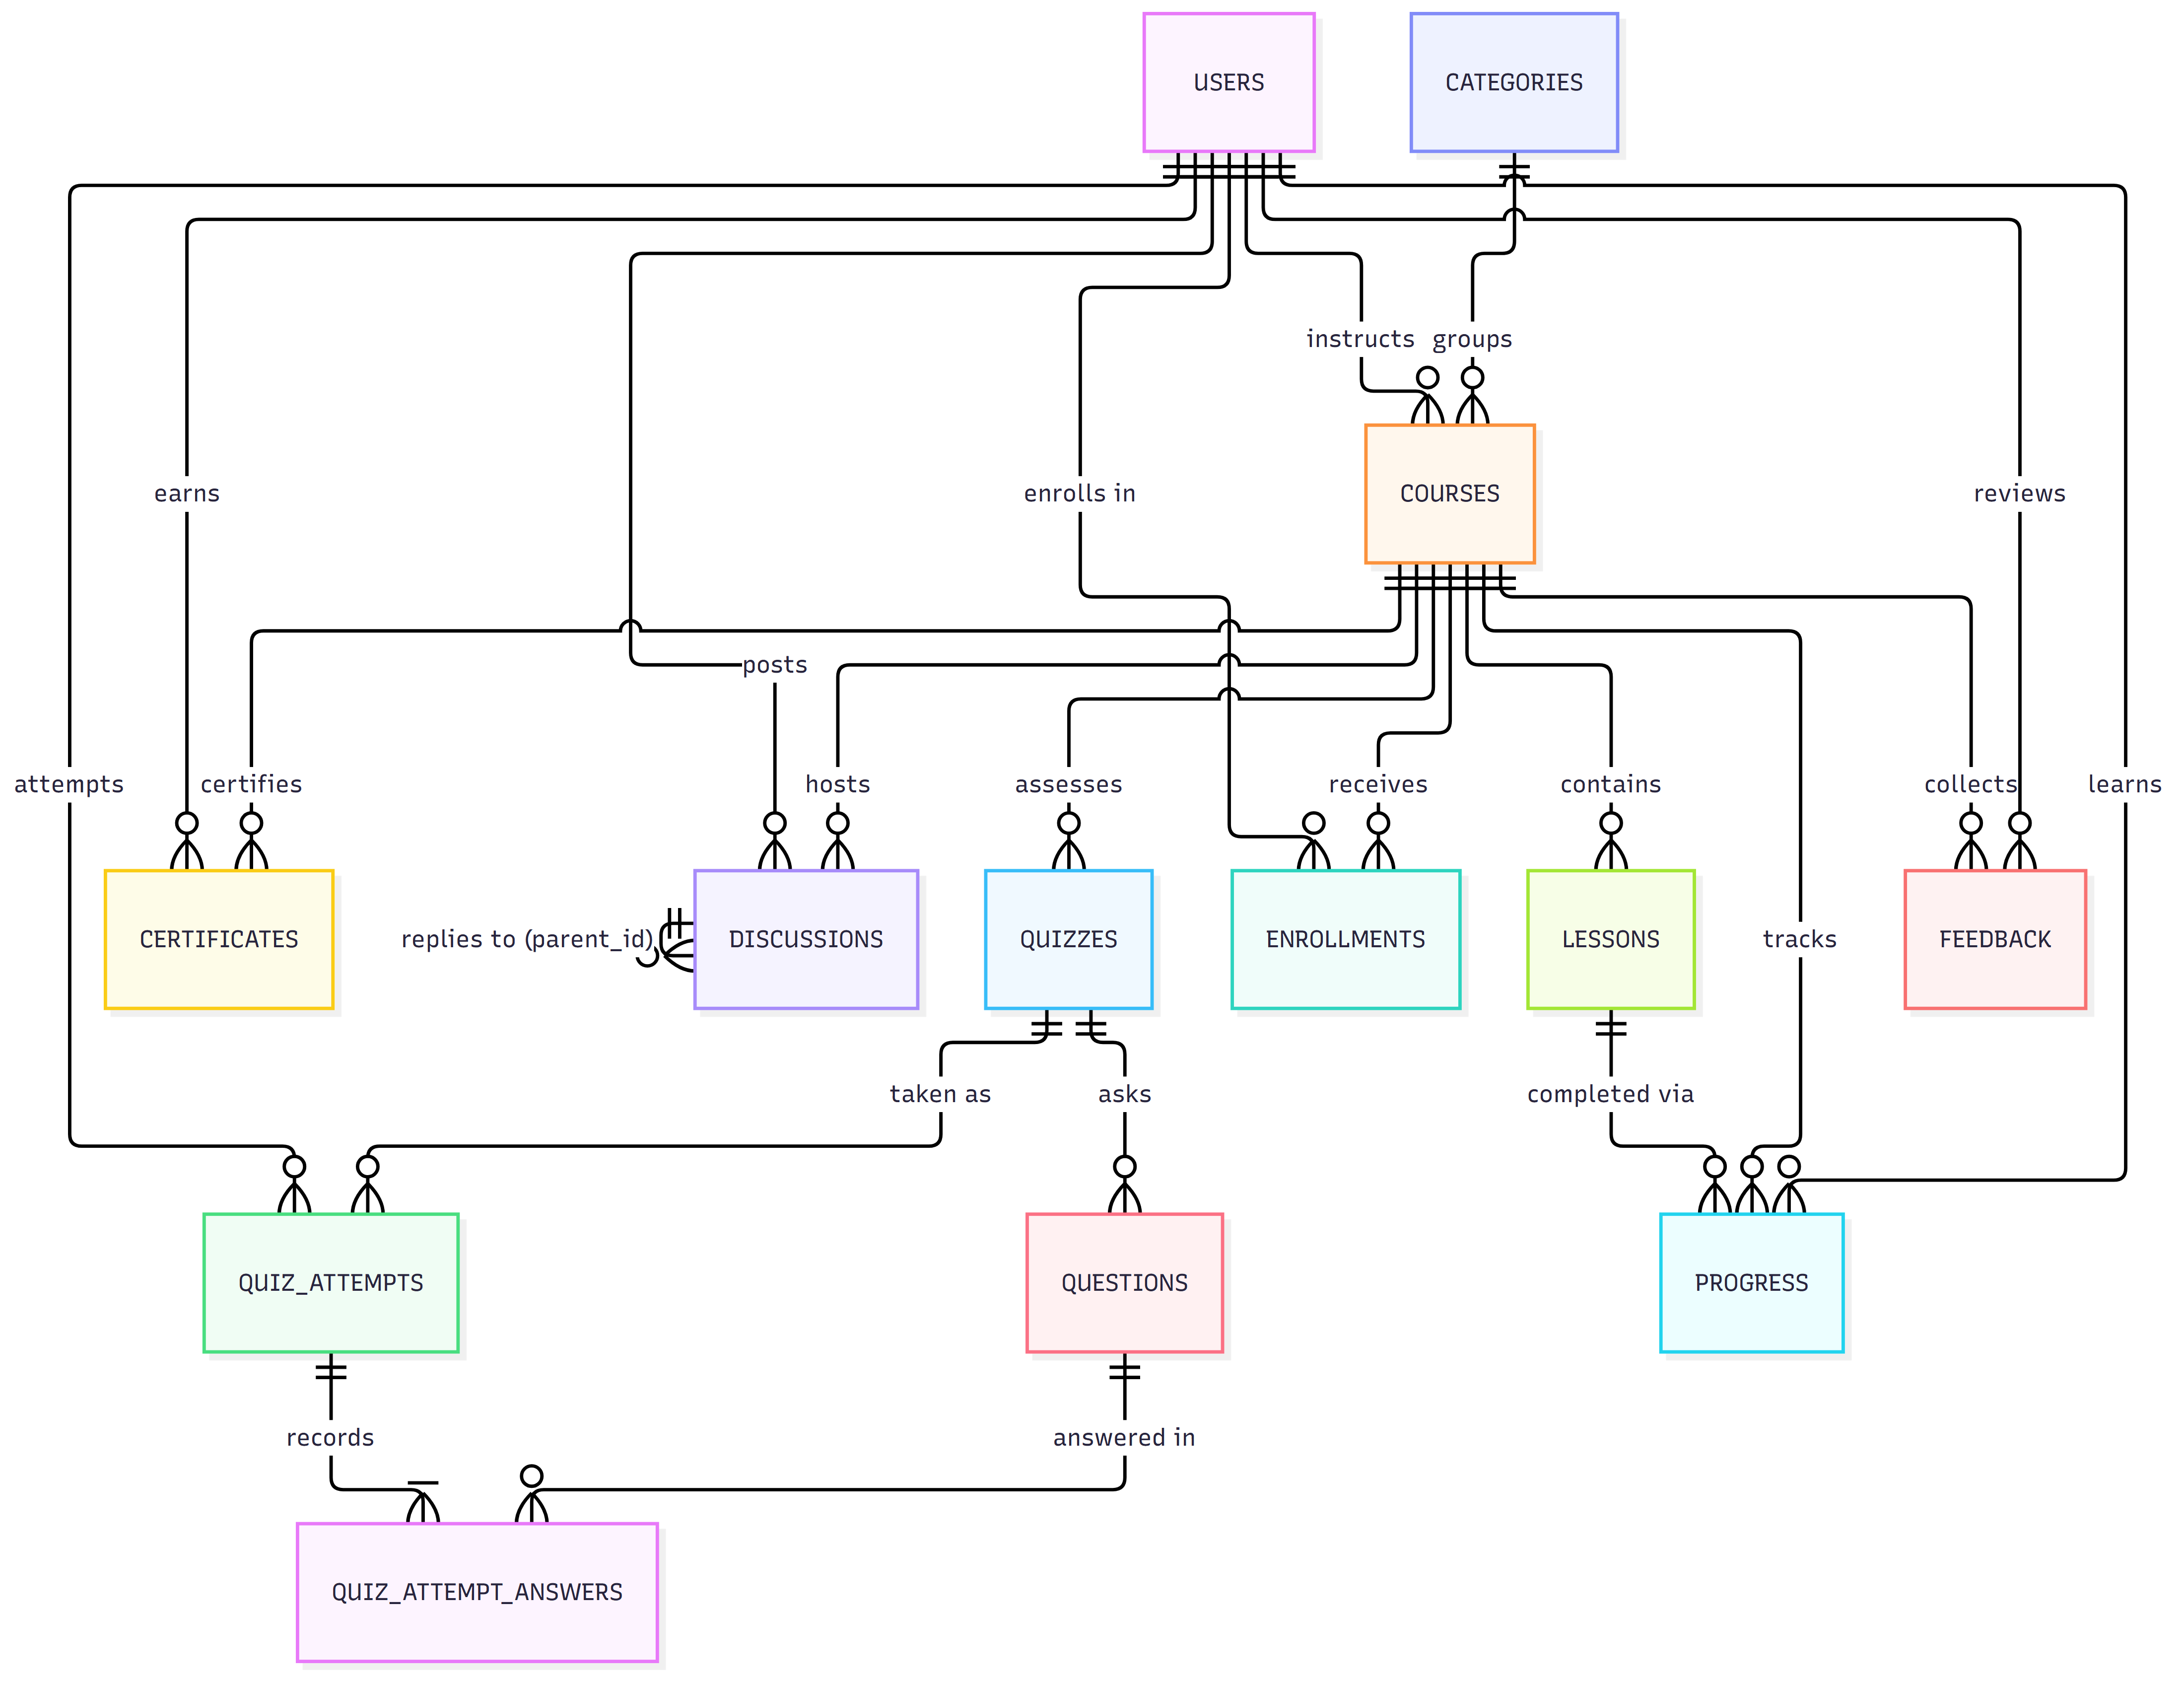
\includegraphics[width=\textwidth]{diagrams/database-er.png}
    \caption{Entity-relationship diagram of the 13 LMS tables}
    \label{fig:database-er}
\end{figure}

\subsection{Tables}
\status{IMPLEMENTED}

\subsubsection{users}
\begin{lstlisting}[language=sql,caption={users table (database/schema.sql)}]
id BIGINT PK AUTO_INCREMENT
name VARCHAR(100) NOT NULL
email VARCHAR(150) NOT NULL UNIQUE          -- idx_users_email
password VARCHAR(255) NOT NULL              -- BCrypt hash
role VARCHAR(30) NOT NULL DEFAULT 'LEARNER' -- idx_users_role
bio TEXT NULL
avatar_url VARCHAR(512) NULL
created_at, updated_at TIMESTAMP NOT NULL DEFAULT CURRENT_TIMESTAMP
\end{lstlisting}

\subsubsection{categories}
\begin{lstlisting}[language=sql]
id BIGINT PK
name VARCHAR(100) NOT NULL UNIQUE
description TEXT NULL
created_at, updated_at TIMESTAMP ...
\end{lstlisting}

\subsubsection{courses}
\begin{lstlisting}[language=sql]
id BIGINT PK
title VARCHAR(255) NOT NULL
description TEXT NULL
category_id BIGINT NULL  -> categories(id) ON DELETE SET NULL   -- fk_courses_category
instructor_id BIGINT NOT NULL -> users(id) ON DELETE CASCADE   -- fk_courses_instructor
status VARCHAR(30) NOT NULL DEFAULT 'DRAFT'                    -- idx_courses_status
thumbnail_url VARCHAR(512) NULL
-- indexes: idx_courses_instructor, idx_courses_category
\end{lstlisting}

\subsubsection{lessons}
\begin{lstlisting}[language=sql]
id BIGINT PK
course_id BIGINT NOT NULL -> courses(id) ON DELETE CASCADE      -- fk_lessons_course
title VARCHAR(255) NOT NULL
description TEXT NULL
content_url VARCHAR(512) NULL        -- video / external resource
content_text LONGTEXT NULL           -- written lesson body
order_index INT NOT NULL DEFAULT 1   -- idx_lessons_order (course_id, order_index)
duration_minutes INT NOT NULL DEFAULT 0
created_at, updated_at TIMESTAMP ...
\end{lstlisting}

\subsubsection{enrollments}
\begin{lstlisting}[language=sql]
id BIGINT PK
user_id BIGINT NOT NULL -> users(id) ON DELETE CASCADE
course_id BIGINT NOT NULL -> courses(id) ON DELETE CASCADE
status VARCHAR(30) NOT NULL DEFAULT 'ENROLLED'  -- ENROLLED|COMPLETED|DROPPED
enrolled_at TIMESTAMP NOT NULL DEFAULT CURRENT_TIMESTAMP
completed_at TIMESTAMP NULL
UNIQUE KEY uk_user_course_enrollment (user_id, course_id)
-- indexes: idx_enrollments_user, idx_enrollments_course, idx_enrollments_status
\end{lstlisting}

\subsubsection{progress}
\begin{lstlisting}[language=sql]
id BIGINT PK
user_id BIGINT NOT NULL -> users(id) ON DELETE CASCADE
course_id BIGINT NOT NULL -> courses(id) ON DELETE CASCADE
lesson_id BIGINT NOT NULL -> lessons(id) ON DELETE CASCADE
completed BOOLEAN NOT NULL DEFAULT FALSE
watch_time_seconds INT NOT NULL DEFAULT 0
completion_percentage DOUBLE NOT NULL DEFAULT 0.0
updated_at TIMESTAMP ...
UNIQUE KEY uk_user_lesson_progress (user_id, lesson_id)
INDEX idx_progress_user_course (user_id, course_id)
\end{lstlisting}

\subsubsection{quizzes}
\begin{lstlisting}[language=sql]
id BIGINT PK
course_id BIGINT NOT NULL -> courses(id) ON DELETE CASCADE
title VARCHAR(255) NOT NULL
description TEXT NULL
passing_score INT NOT NULL DEFAULT 70
time_limit_minutes INT NOT NULL DEFAULT 30
created_at, updated_at TIMESTAMP ...
INDEX idx_quizzes_course (course_id)
\end{lstlisting}

\subsubsection{questions}
\begin{lstlisting}[language=sql]
id BIGINT PK
quiz_id BIGINT NOT NULL -> quizzes(id) ON DELETE CASCADE
question_text TEXT NOT NULL
option_a..option_d VARCHAR(500) NOT NULL      -- four fixed options
correct_option VARCHAR(10) NOT NULL           -- 'A'..'D'
points INT NOT NULL DEFAULT 10
explanation TEXT NULL
created_at, updated_at TIMESTAMP ...
INDEX idx_questions_quiz (quiz_id)
\end{lstlisting}

\subsubsection{quiz\_attempts} and \subsubsection{quiz\_attempt\_answers}
\begin{lstlisting}[language=sql]
quiz_attempts:
  id BIGINT PK
  quiz_id BIGINT NOT NULL -> quizzes(id) ON DELETE CASCADE
  user_id BIGINT NOT NULL -> users(id) ON DELETE CASCADE
  score INT DEFAULT 0, total_points INT DEFAULT 0, passed BOOLEAN DEFAULT FALSE
  started_at TIMESTAMP NOT NULL, submitted_at TIMESTAMP NULL
  indexes: idx_quiz_attempts_user, idx_quiz_attempts_quiz

quiz_attempt_answers:
  id BIGINT PK
  attempt_id BIGINT NOT NULL -> quiz_attempts(id) ON DELETE CASCADE
  question_id BIGINT NOT NULL -> questions(id) ON DELETE CASCADE
  selected_option VARCHAR(10) NOT NULL
  is_correct BOOLEAN DEFAULT FALSE, points_awarded INT DEFAULT 0
  index: idx_attempt_answers_attempt
\end{lstlisting}

\subsubsection{discussions}
\begin{lstlisting}[language=sql]
id BIGINT PK
course_id BIGINT NOT NULL -> courses(id) ON DELETE CASCADE
user_id BIGINT NOT NULL -> users(id) ON DELETE CASCADE
parent_id BIGINT NULL -> discussions(id) ON DELETE CASCADE   -- self reference (threads/replies)
title VARCHAR(255) NULL       -- NULL for replies
content TEXT NOT NULL
created_at, updated_at TIMESTAMP ...
indexes: idx_discussions_course, idx_discussions_parent
\end{lstlisting}

\subsubsection{feedback}
\begin{lstlisting}[language=sql]
id BIGINT PK
course_id BIGINT NOT NULL -> courses(id) ON DELETE CASCADE
user_id BIGINT NOT NULL -> users(id) ON DELETE CASCADE
rating INT NOT NULL CHECK (rating >= 1 AND rating <= 5)
comment TEXT NULL
created_at, updated_at TIMESTAMP ...
UNIQUE KEY uk_user_course_feedback (user_id, course_id)
INDEX idx_feedback_course (course_id)
\end{lstlisting}

\subsubsection{certificates}
\begin{lstlisting}[language=sql]
id BIGINT PK
certificate_code VARCHAR(64) NOT NULL UNIQUE    -- idx_certificates_code
user_id BIGINT NOT NULL -> users(id) ON DELETE CASCADE
course_id BIGINT NOT NULL -> courses(id) ON DELETE CASCADE
issue_date TIMESTAMP NOT NULL DEFAULT CURRENT_TIMESTAMP
grade VARCHAR(50) DEFAULT 'PASS'                -- runtime value is 'DISTINCTION'
certificate_url VARCHAR(512) NULL               -- API path to the certificate
UNIQUE KEY uk_user_course_certificate (user_id, course_id)
\end{lstlisting}

\subsection{Relationship summary}
\status{IMPLEMENTED}

\begin{table}[H]
\centering
\caption{Foreign-key relationships and cardinalities}
\label{tab:relationships}
\begin{tabular}{@{}L{3.6cm}L{3.6cm}C{2.4cm}L{4.0cm}@{}}
\toprule
\textbf{Child} & \textbf{Parent} & \textbf{Cardinality} & \textbf{On delete} \\
\midrule
courses.category\_id & categories & optional many--one & SET NULL \\
courses.instructor\_id & users & many--one (required) & CASCADE \\
lessons.course\_id & courses & many--one & CASCADE \\
enrollments.user\_id / course\_id & users / courses & many--many (associative) & CASCADE \\
progress.user\_id / course\_id / lesson\_id & users / courses / lessons & many--one per dimension & CASCADE \\
quizzes.course\_id & courses & many--one & CASCADE \\
questions.quiz\_id & quizzes & many--one & CASCADE \\
quiz\_attempts.quiz\_id / user\_id & quizzes / users & many--one & CASCADE \\
quiz\_attempt\_answers.attempt\_id / question\_id & quiz\_attempts / questions & many--one & CASCADE \\
discussions.parent\_id & discussions & self (thread/reply) & CASCADE \\
feedback.course\_id / user\_id & courses / users & many--one & CASCADE \\
certificates.user\_id / course\_id & users / courses & many--one & CASCADE \\
\bottomrule
\end{tabular}
\end{table}

\subsection{Indexes and constraints}
\status{IMPLEMENTED}

\begin{itemize}
    \item \textbf{20 secondary indexes} declared in \pathref{database/schema.sql} (email, role, instructor, category, status, course lookups, user/course pairs, attempt/answer lookups, discussion parent, certificate code).
    \item \textbf{4 unique business keys:} \code{uk_user_course_enrollment}, \code{uk_user_lesson_progress}, \code{uk_user_course_feedback}, \code{uk_user_course_certificate} -- these enforce ``one enrolment / one progress row / one review / one certificate'' at the database level.
    \item \textbf{Check constraint:} \code{feedback.rating} between 1 and 5 (schema-level; additionally enforced by \code{@Min(1)}/\code{@Max(5)} on the DTO).
    \item \textbf{Referential deletion:} child rows cascade with their parents; removing a category only detaches courses.
\end{itemize}

\subsection{Views, stored procedures, functions, triggers}
\status{NOT APPLICABLE (verified)}

\pathref{database/schema.sql} contains no \code{VIEW}, \code{PROCEDURE}, \code{FUNCTION} or \code{TRIGGER} statements; all derived values (progress percentages, counts, scores) are computed in the application layer.

\subsection{Row-level security and database access control}
\status{NOT IMPLEMENTED / NOT APPLICABLE}

MySQL has no RLS feature; the repository configures no dedicated database roles or grants (the app connects with credentials from the datasource configuration, defaulting to \code{root}). All row-level enforcement happens in Java services. \status{RECOMMENDED} a least-privilege application DB user for production.

\subsection{Migrations and schema evolution}
\status{PARTIAL}

\begin{itemize}
    \item No Flyway or Liquibase dependency exists in \pathref{backend/pom.xml}; there are no versioned migration files.
    \item Schema is created by \pathref{database/schema.sql} (manual import, documented in \pathref{README.md}) and then kept in sync by Hibernate \code{ddl-auto: update}, which can add tables/columns but never alters or drops them.
    \item \pathref{database/seed.sql} and \pathref{database/dummy.sql} provide \code{INSERT IGNORE} sample data (demo users with BCrypt hash for \code{password123}, 2--3 sample courses, lessons, quizzes, questions).
\end{itemize}
\noindent \textbf{Risk:} schema drift between hand-written SQL and entity definitions is possible and untested in CI (no pipeline). See Section~\ref{sec:technical-debt}.

\subsection{Entity/schema parity notes}
\status{IMPLEMENTED (observations)}

\begin{itemize}
    \item All 13 \code{@Entity} classes map one-to-one to the 13 tables (verified: \code{@Table} names match).
    \item The runtime \code{grade} value written by \code{CertificateService} is \code{DISTINCTION} while the column default is \code{PASS} -- cosmetic inconsistency documented in Section~\ref{sec:known-issues}.
    \item The \code{progress} table has no \code{created_at} (only \code{updated_at}) -- matches the entity.
\end{itemize}

\section{API Documentation}
\label{sec:api-documentation}

\subsection{Base conventions}
\status{IMPLEMENTED}

All REST endpoints are versioned under \code{/api/v1}. JSON request/response bodies use DTOs in \pathref{backend/src/main/java/com/example/lms/dto/}. Success envelopes use \pathref{backend/src/main/java/com/example/lms/dto/response/ApiResponse.java}; errors use \pathref{backend/src/main/java/com/example/lms/dto/response/ErrorResponse.java}. Interactive docs are served by springdoc-openapi 2.6.0 (\pathref{backend/src/main/java/com/example/lms/config/OpenApiConfig.java}): OpenAPI JSON at \code{/v3/api-docs} and Swagger UI at \code{/swagger-ui.html} or \code{/swagger-ui/index.html}.

\subsection{Endpoint inventory (47 mapped endpoints, 11 controllers)}
\status{IMPLEMENTED}

\begin{table}[H]
\centering
\caption{Controller to endpoint-group mapping (verified in controller sources)}
\label{tab:api-inventory}
\begin{tabular}{@{}L{3.8cm}L{9.4cm}@{}}
\toprule
\textbf{Controller} & \textbf{Endpoints} \\
\midrule
\pathref{controller/AuthController.java} & \code{POST /api/v1/auth/register}, \code{POST /api/v1/auth/login}, \code{POST /api/v1/auth/logout} \\
\pathref{controller/UserController.java} & \code{GET /api/v1/users}, \code{GET /api/v1/users/\{id\}}, \code{PUT /api/v1/users/\{id\}} \\
\pathref{controller/CourseController.java} & \code{GET /api/v1/courses}, \code{GET /api/v1/courses/\{id\}}, \code{POST /api/v1/courses}, \code{PUT /api/v1/courses/\{id\}}, \code{DELETE /api/v1/courses/\{id\}} \\
\pathref{controller/EnrollmentController.java} & \code{POST /api/v1/courses/\{courseId\}/enroll}, \code{DELETE /api/v1/courses/\{courseId\}/enroll}, \code{GET /api/v1/users/\{userId\}/enrollments} \\
\pathref{controller/LessonController.java} & \code{GET /api/v1/courses/\{courseId\}/lessons}, \code{GET /api/v1/lessons/\{lessonId\}}, \code{POST /api/v1/courses/\{courseId\}/lessons}, \code{PUT /api/v1/lessons/\{lessonId\}}, \code{DELETE /api/v1/lessons/\{lessonId\}} \\
\pathref{controller/ProgressController.java} & \code{GET /api/v1/courses/\{courseId\}/progress}, \code{POST /api/v1/lessons/\{lessonId\}/progress}, \code{PATCH /api/v1/lessons/\{lessonId\}/progress} \\
\pathref{controller/QuizController.java} & Quiz CRUD plus \code{POST /api/v1/quizzes/\{quizId\}/attempts}, \code{GET /api/v1/quizzes/\{quizId\}/results} \\
\pathref{controller/DiscussionController.java} & \code{GET/POST /api/v1/courses/\{courseId\}/discussions}, replies, delete \\
\pathref{controller/FeedbackController.java} & \code{GET/POST /api/v1/courses/\{courseId\}/feedback}, \code{PUT /api/v1/feedback/\{feedbackId\}} \\
\pathref{controller/CertificateController.java} & \code{GET/POST /api/v1/courses/\{courseId\}/certificate} \\
\pathref{controller/CategoryController.java} & Category CRUD under \code{/api/v1/categories} \\
\bottomrule
\end{tabular}
\end{table}

\subsection{Error model}
\status{IMPLEMENTED}

Canonical codes: \code{VALIDATION_ERROR} (400), \code{UNAUTHORIZED} (401), \code{FORBIDDEN} (403), \code{RESOURCE_NOT_FOUND} (404), \code{RESOURCE_CONFLICT} (409, e.g.\ duplicate enrollment), \code{INVALID_OPERATION} (422), \code{INTERNAL_SERVER_ERROR} (500). Stack traces and credentials are never returned. The frontend normalises these in \pathref{frontend/src/api/client.js}.

\section{Authentication}
\label{sec:authentication}

\subsection{Mechanism}
\status{IMPLEMENTED}

Stateless JWT authentication. Registration and login are handled by \pathref{backend/src/main/java/com/example/lms/controller/AuthController.java} and \pathref{backend/src/main/java/com/example/lms/service/AuthService.java}. Passwords are hashed with BCrypt; on success the backend issues a signed JWT (JJWT 0.12.6, secret \code{JWT_SECRET}, expiry \code{JWT_EXPIRATION=86400000} per \pathref{.env.example}). The frontend stores the token in \code{localStorage} (\pathref{frontend/src/context/AuthContext.jsx}) and attaches \code{Authorization: Bearer <token>} via an Axios interceptor (\pathref{frontend/src/api/client.js}).

\begin{figure}[H]
\centering
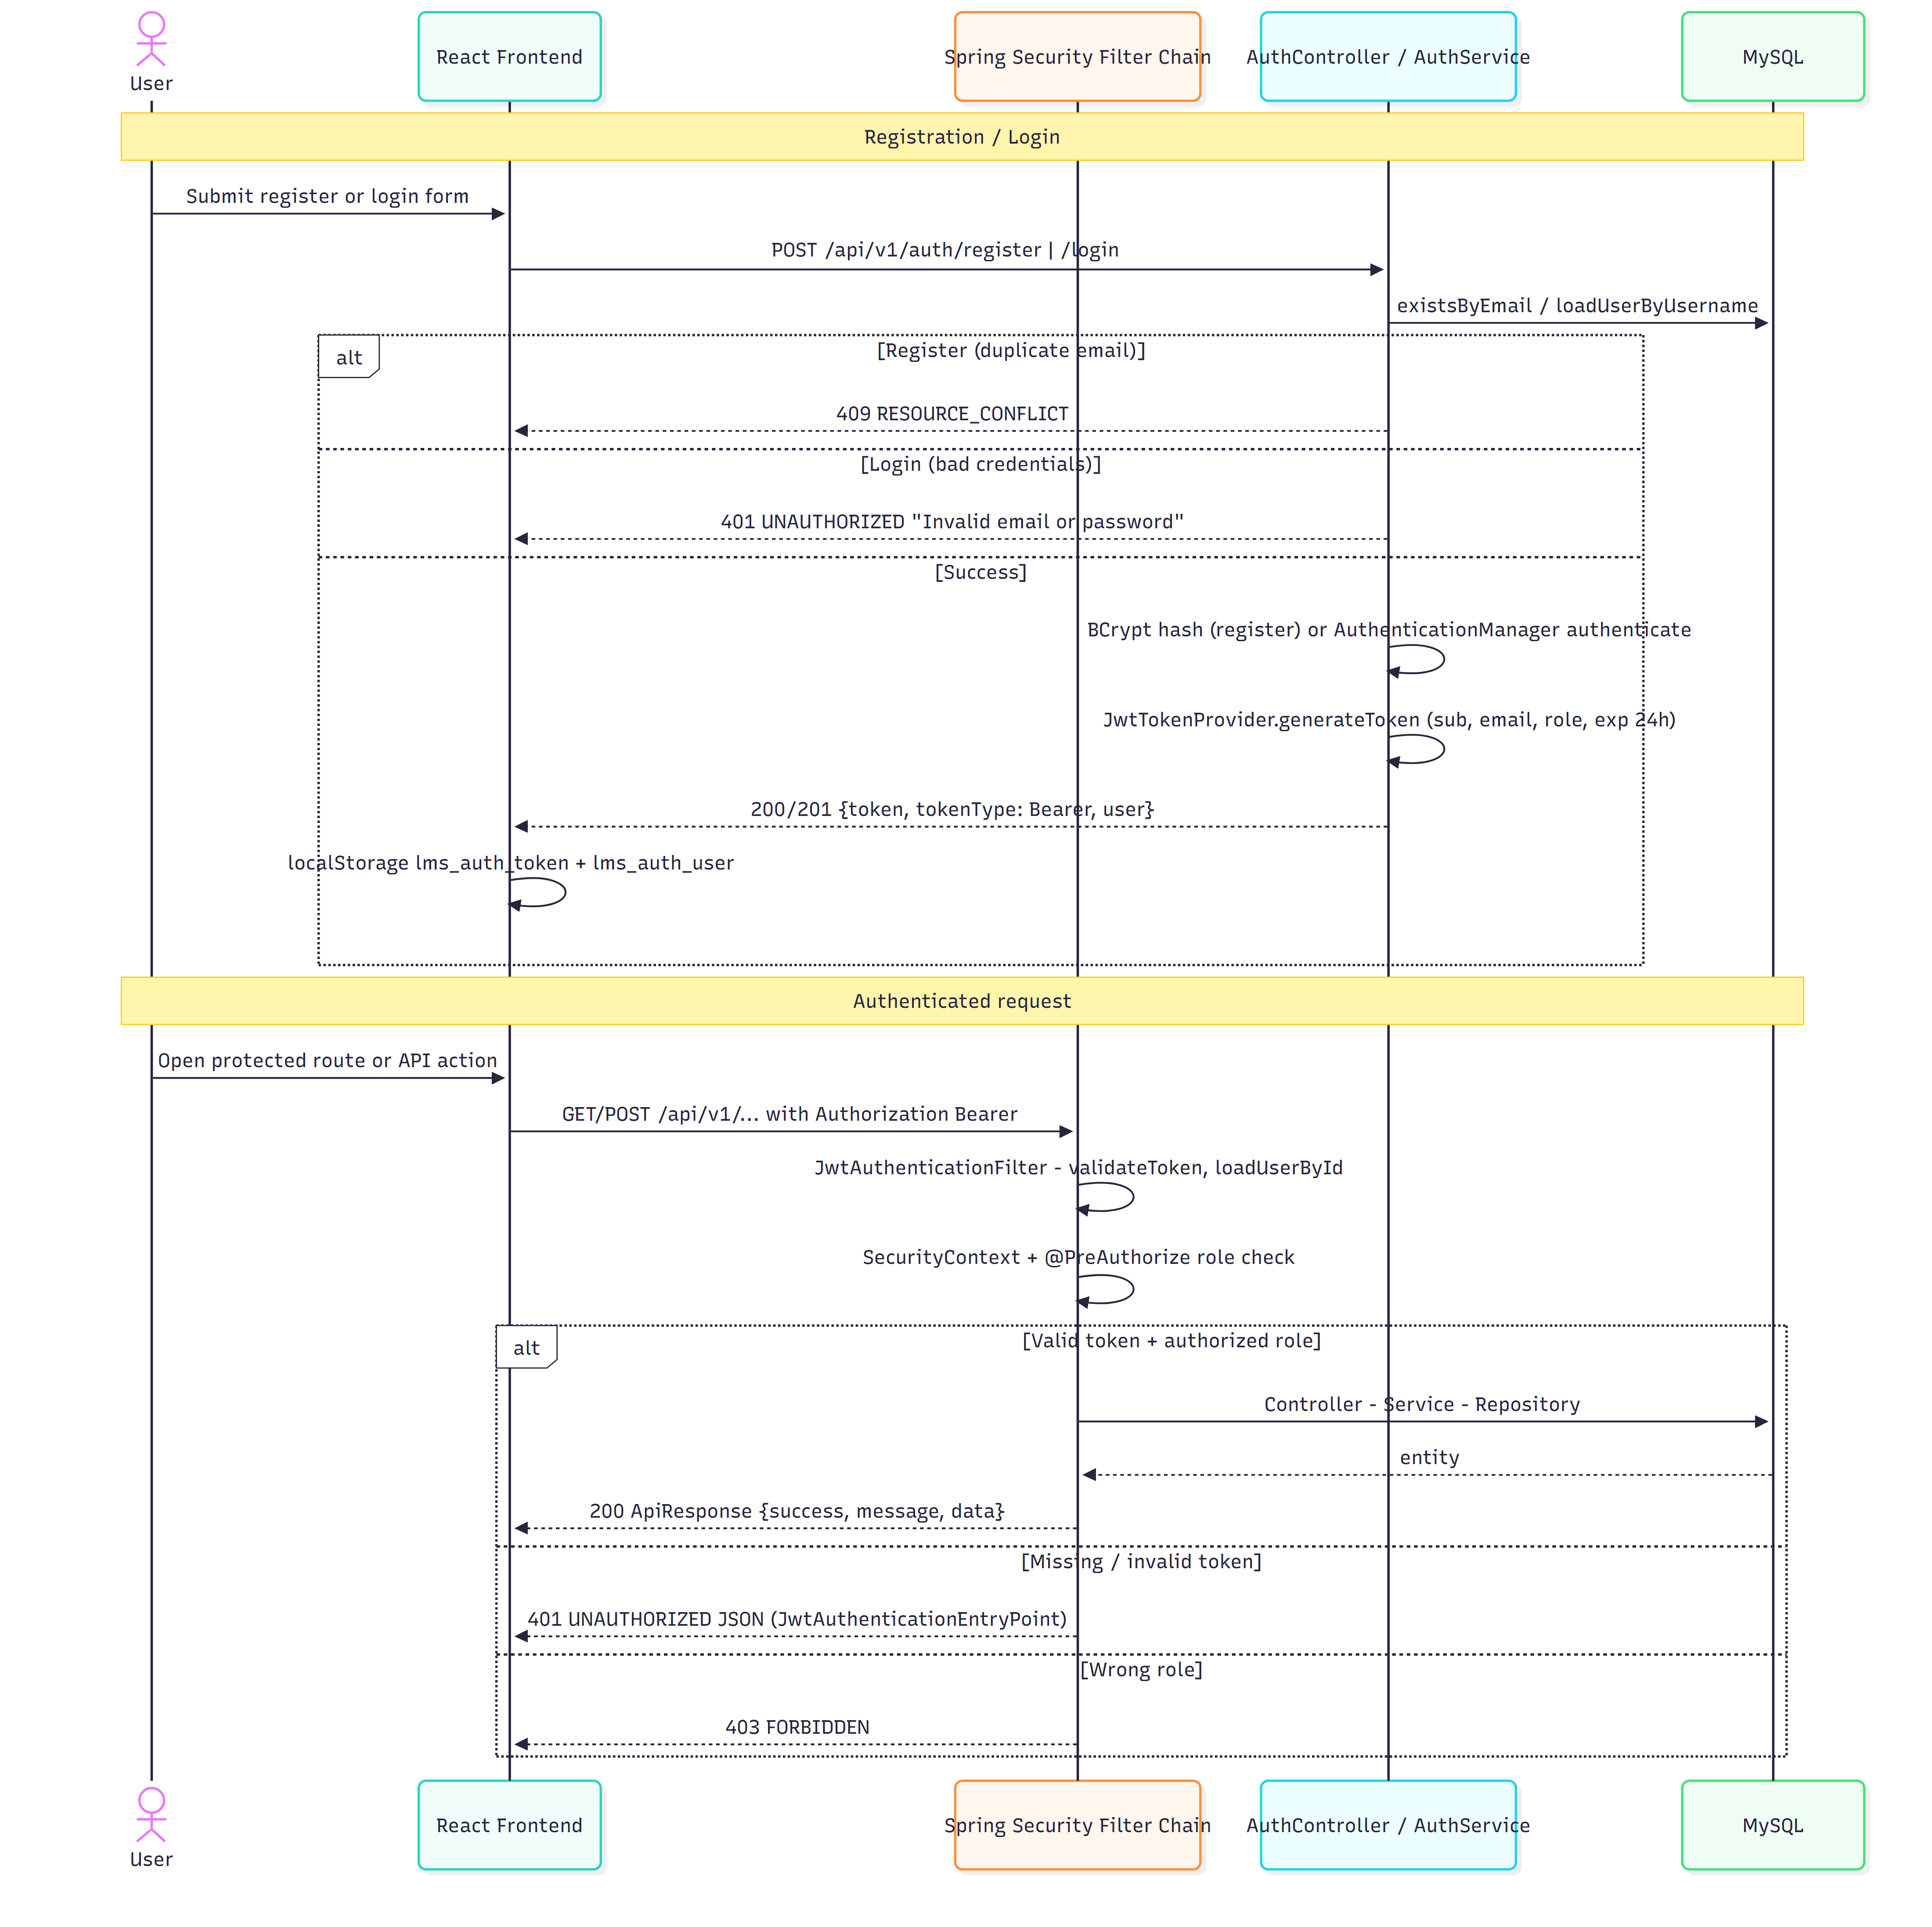
\includegraphics[width=0.95\textwidth]{diagrams/authentication-flow.png}
\caption{Authentication flow -- register, login, JWT issuance, per-request validation}
\label{fig:auth-flow-detail}
\end{figure}

\subsection{Validation chain}
\status{IMPLEMENTED}

Every request passes through the Spring Security filter chain (\pathref{backend/src/main/java/com/example/lms/config/SecurityConfig.java} plus \pathref{backend/src/main/java/com/example/lms/security/}): token signature and expiry are validated, the user principal is loaded, and method-level rules are applied. Invalid or expired tokens yield 401. There is no server-side session store and no token revocation list -- logout is client-side token removal plus a \code{POST /api/v1/auth/logout} acknowledgement.

\subsection{Limitations}
\status{IMPLEMENTED (gaps recorded)}

No password recovery, no email verification, no refresh-token rotation, and no lockout after repeated failures. Seed users created by \pathref{backend/src/main/java/com/example/lms/config/DataInitializer.java} use hardcoded passwords (finding S-02, Section~\ref{sec:security}).

\section{Authorization}
\label{sec:authorization}

\subsection{Model}
\status{IMPLEMENTED}

Role-based access control with three roles stored in \code{users.role} (\pathref{database/schema.sql}, default \code{LEARNER}): \code{LEARNER}, \code{INSTRUCTOR}, \code{ADMIN}. Enforcement is server-side via Spring Security method annotations; the frontend mirrors the same rules for UX only through \pathref{frontend/src/routes/ProtectedRoute.jsx} and \pathref{frontend/src/routes/AppRoutes.jsx} (route guards are not a security boundary -- CONTRACT.md section 13).

\subsection{Authorization matrix}
\status{IMPLEMENTED}

\begin{table}[H]
\centering
\caption{Authorization matrix (backend-enforced; frontend mirrors for UX)}
\label{tab:authz-matrix}
\begin{tabular}{@{}L{5.2cm}C{2.2cm}C{2.2cm}C{2.2cm}@{}}
\toprule
\textbf{Feature} & \textbf{Learner} & \textbf{Instructor} & \textbf{Admin} \\
\midrule
Browse / view courses & Yes & Yes & Yes \\
Enroll in courses & Yes & -- & Yes \\
Access lessons / track own progress & Yes & Yes (own) & Yes \\
Take quiz / view own results & Yes & -- & Yes \\
Create / edit / delete own course & -- & Yes & Yes \\
Manage questions and quizzes & -- & Yes & Yes \\
View learner performance & -- & Yes (own courses) & Yes \\
Participate in discussions & Yes & Yes & Yes \\
Submit feedback & Yes & -- & -- \\
Manage users / instructors / all courses & -- & -- & Yes \\
Access admin dashboard & -- & -- & Yes \\
\bottomrule
\end{tabular}
\end{table}

\noindent Ownership checks (e.g.\ instructor may modify only own courses) are performed in service-layer code. Known service-level gaps are recorded as PARTIAL in Section~\ref{sec:security}.

\section{User Flows}
\label{sec:user-flows}

\subsection{Covered flows}
\status{IMPLEMENTED}

The end-to-end backend test \pathref{backend/src/test/java/com/example/lms/integration/LmsIntegrationTest.java} exercises the canonical flows: register $\rightarrow$ login $\rightarrow$ create course $\rightarrow$ add lessons $\rightarrow$ create quiz $\rightarrow$ enroll $\rightarrow$ update progress $\rightarrow$ submit quiz $\rightarrow$ issue certificate $\rightarrow$ post discussion and feedback. Frontend routes for each step live in \pathref{frontend/src/routes/AppRoutes.jsx} (19 routes including \code{/courses}, \code{/courses/:id}, \code{/courses/:courseId/learn}, \code{/quizzes/:id}, \code{/learner}, \code{/instructor}, \code{/admin}, \code{/profile}).

\begin{figure}[H]
\centering
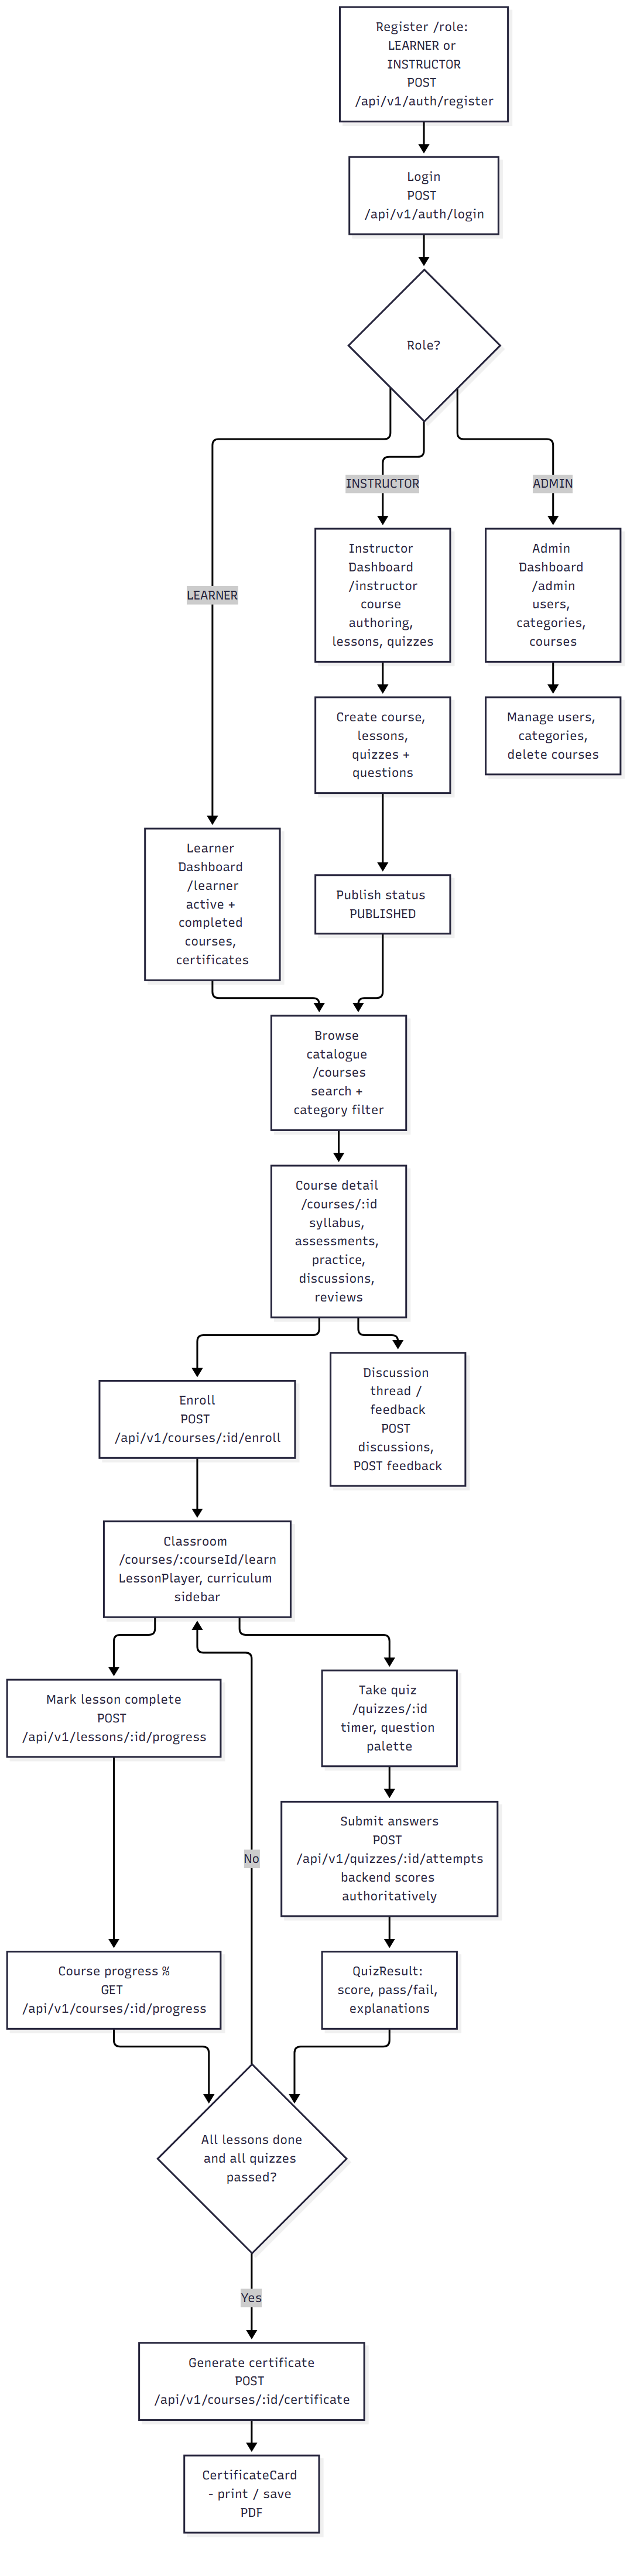
\includegraphics[width=0.86\textwidth]{diagrams/learning-lifecycle.png}
\caption{Learning lifecycle -- registration through certificate}
\label{fig:learning-lifecycle-flows}
\end{figure}

\subsection{Flow details}

\begin{enumerate}
\item \textbf{Registration and login:} \code{/register} $\rightarrow$ \code{POST /api/v1/auth/register} $\rightarrow$ \code{/login} $\rightarrow$ \code{POST /api/v1/auth/login} $\rightarrow$ JWT stored $\rightarrow$ role dashboard.
\item \textbf{Enrollment:} catalogue (\code{/courses}) $\rightarrow$ detail (\code{/courses/:id}) $\rightarrow$ enroll (\code{POST /api/v1/courses/\{courseId\}/enroll}) $\rightarrow$ learn view unlocked. Duplicate enrollment is rejected with 409.
\item \textbf{Learning:} \code{/courses/:courseId/learn} renders \pathref{frontend/src/pages/LearningPage.jsx}; lesson completion posts progress; the dashboard reflects persisted state.
\item \textbf{Assessment:} \code{/quizzes/:id} renders \pathref{frontend/src/pages/QuizTakingPage.jsx}; submission is validated and scored server-side; the result view shows the authoritative score.
\item \textbf{Certificate:} eligibility is verified by \pathref{backend/src/main/java/com/example/lms/service/CertificateService.java}; the learner downloads the certificate from the learner dashboard.
\end{enumerate}

\begin{figure}[H]
\centering
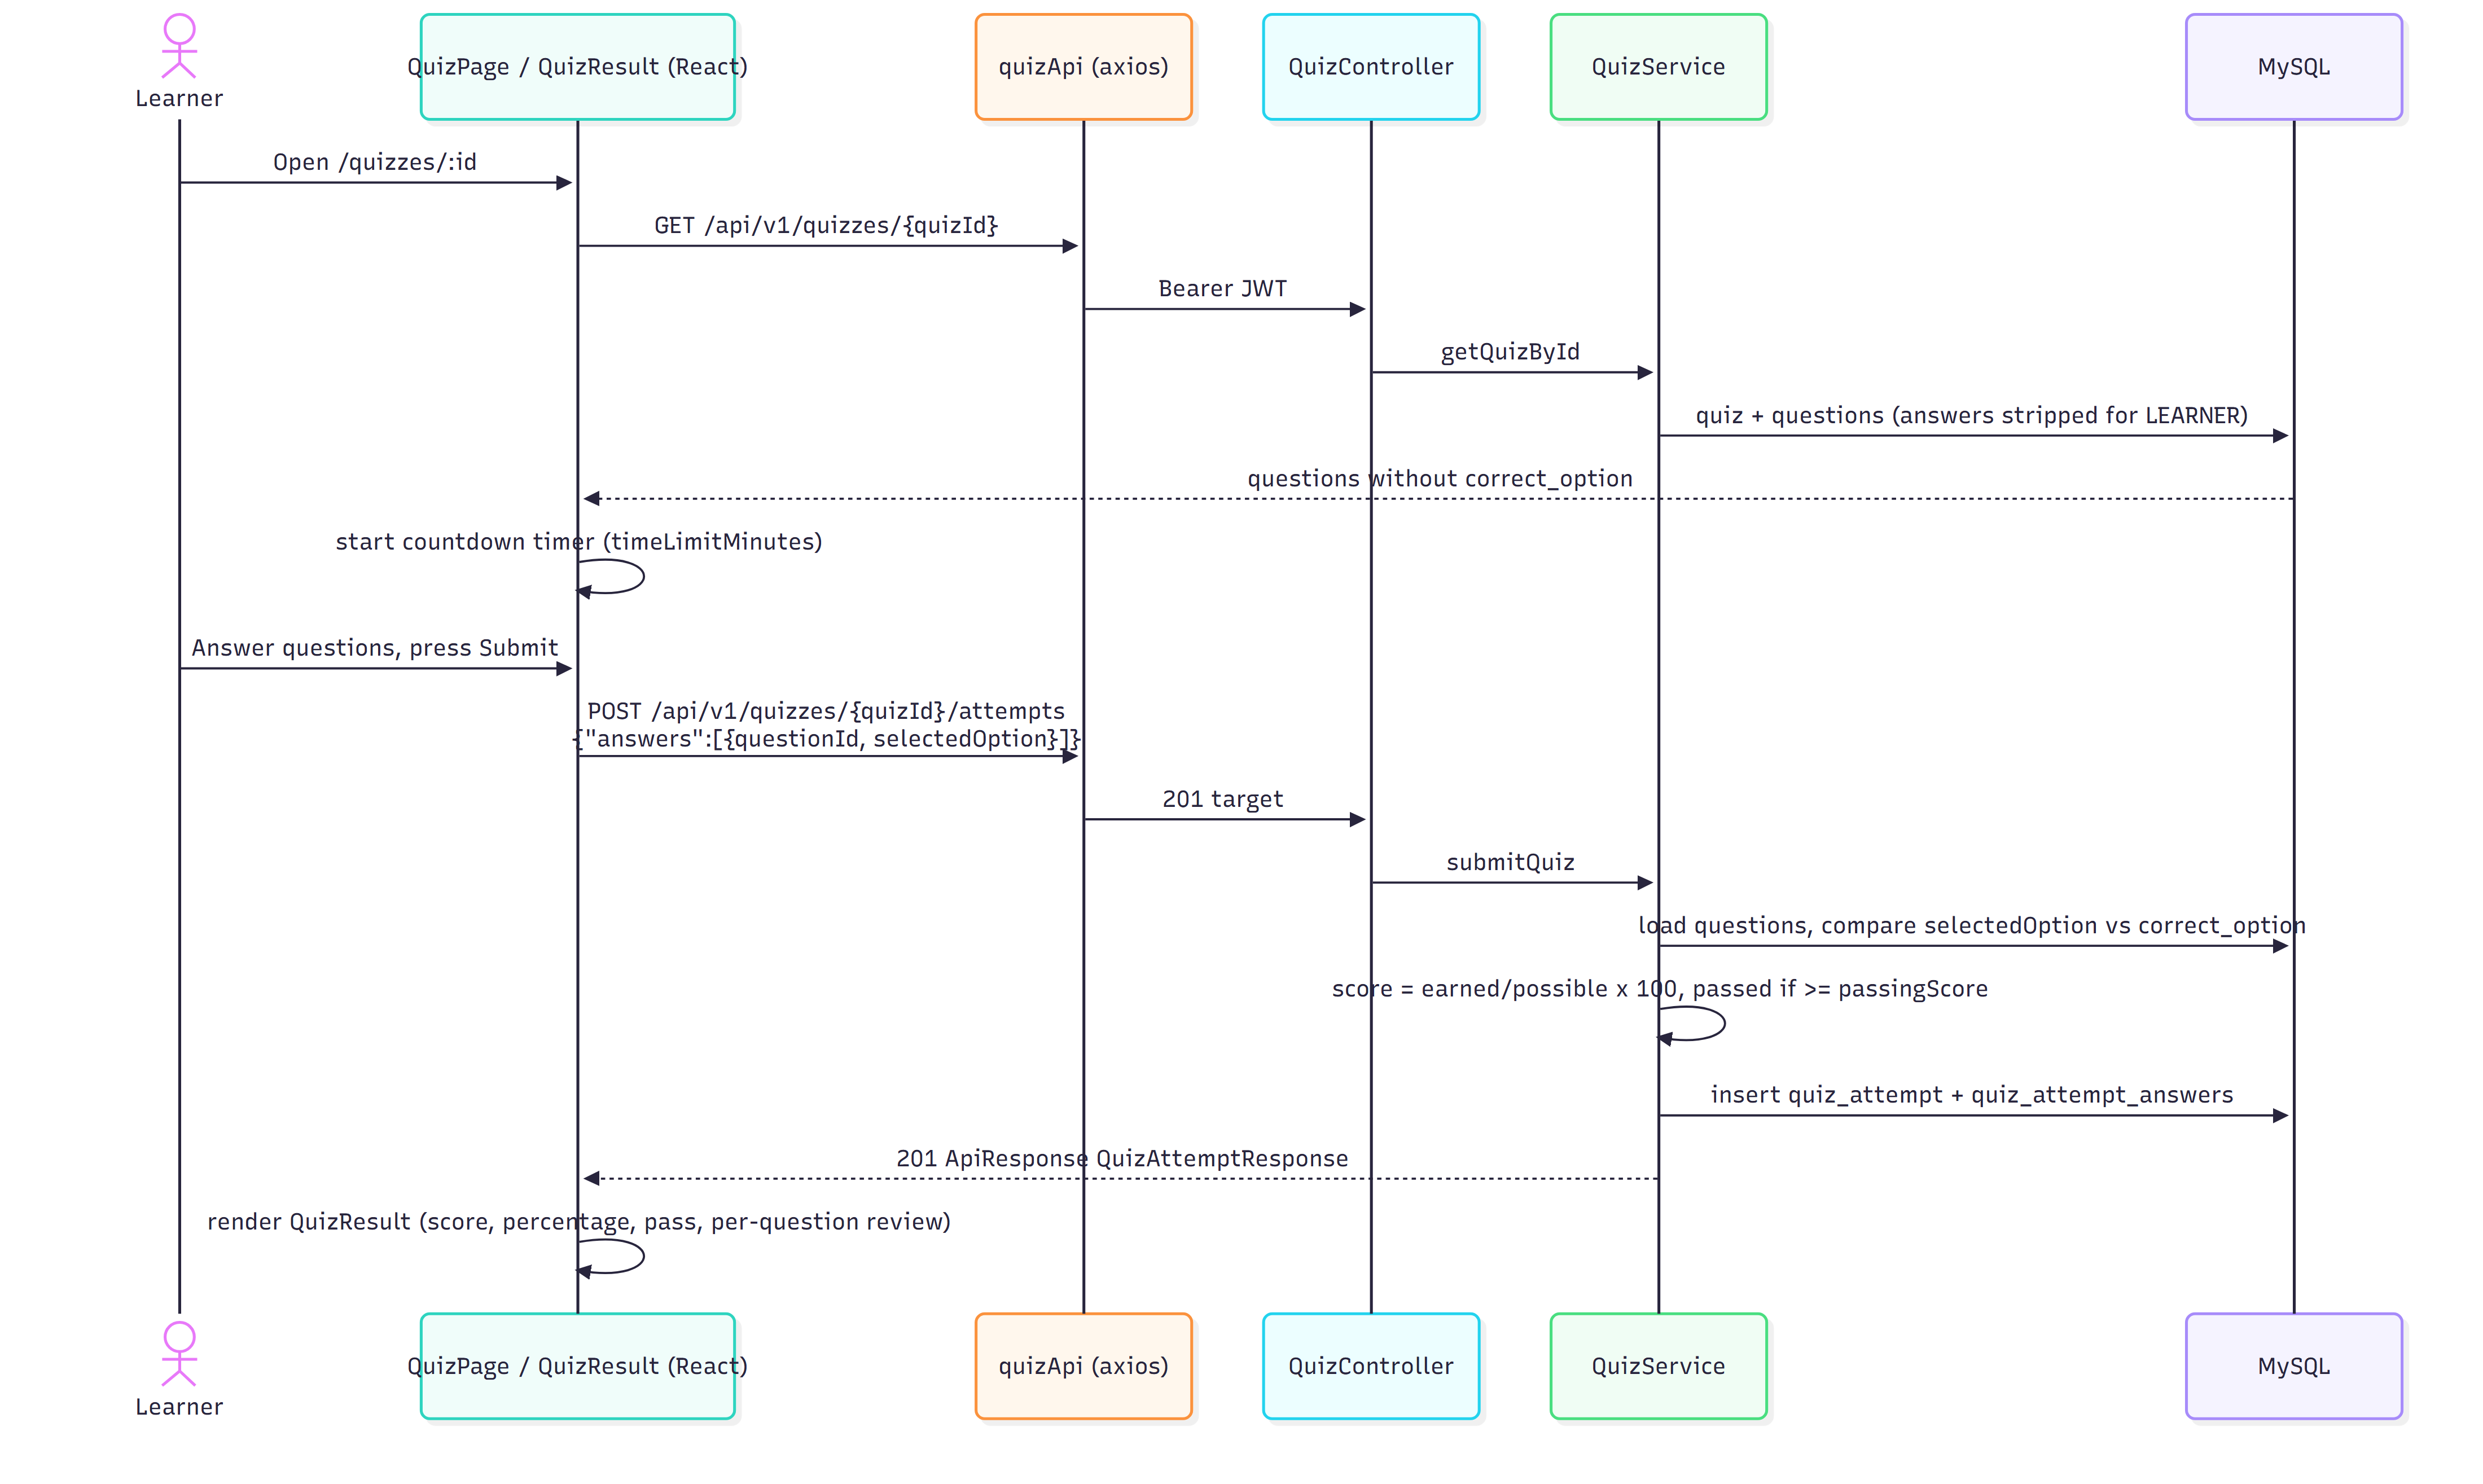
\includegraphics[width=0.95\textwidth]{diagrams/quiz-submission-sequence.png}
\caption{Quiz submission sequence -- client attempt, server validation, persisted result}
\label{fig:quiz-seq}
\end{figure}

\section{Data Flows}
\label{sec:data-flows}

\subsection{Request lifecycle}
\status{IMPLEMENTED}

All interactions are synchronous JSON over HTTP: React component $\rightarrow$ feature API module in \pathref{frontend/src/api/} $\rightarrow$ shared Axios client (\pathref{frontend/src/api/client.js}, base URL from \code{VITE_API_BASE_URL}) $\rightarrow$ Spring Security filter chain $\rightarrow$ controller $\rightarrow$ service (transactional business rules) $\rightarrow$ JPA repository $\rightarrow$ MySQL. Responses return through DTOs; the Axios client unwraps envelopes and maps error codes for display.

\subsection{Key data chains}

\begin{itemize}
\item \textbf{Progress:} lesson completion event $\rightarrow$ \code{POST/PATCH /api/v1/lessons/\{lessonId\}/progress} $\rightarrow$ \pathref{backend/src/main/java/com/example/lms/service/ProgressService.java} $\rightarrow$ \code{progress} table $\rightarrow$ aggregated \pathref{backend/src/main/java/com/example/lms/dto/response/CourseProgressResponse.java}.
\item \textbf{Assessment:} answers $\rightarrow$ \code{POST /api/v1/quizzes/\{quizId\}/attempts} $\rightarrow$ \pathref{backend/src/main/java/com/example/lms/service/QuizService.java} scores server-side $\rightarrow$ attempt/result rows. The frontend is never authoritative for scores.
\item \textbf{Certificate:} completion signal $\rightarrow$ \pathref{backend/src/main/java/com/example/lms/service/CertificateService.java} verifies enrollment, progress and quiz outcome $\rightarrow$ \code{certificates} row $\rightarrow$ download.
\end{itemize}

\begin{figure}[H]
\centering
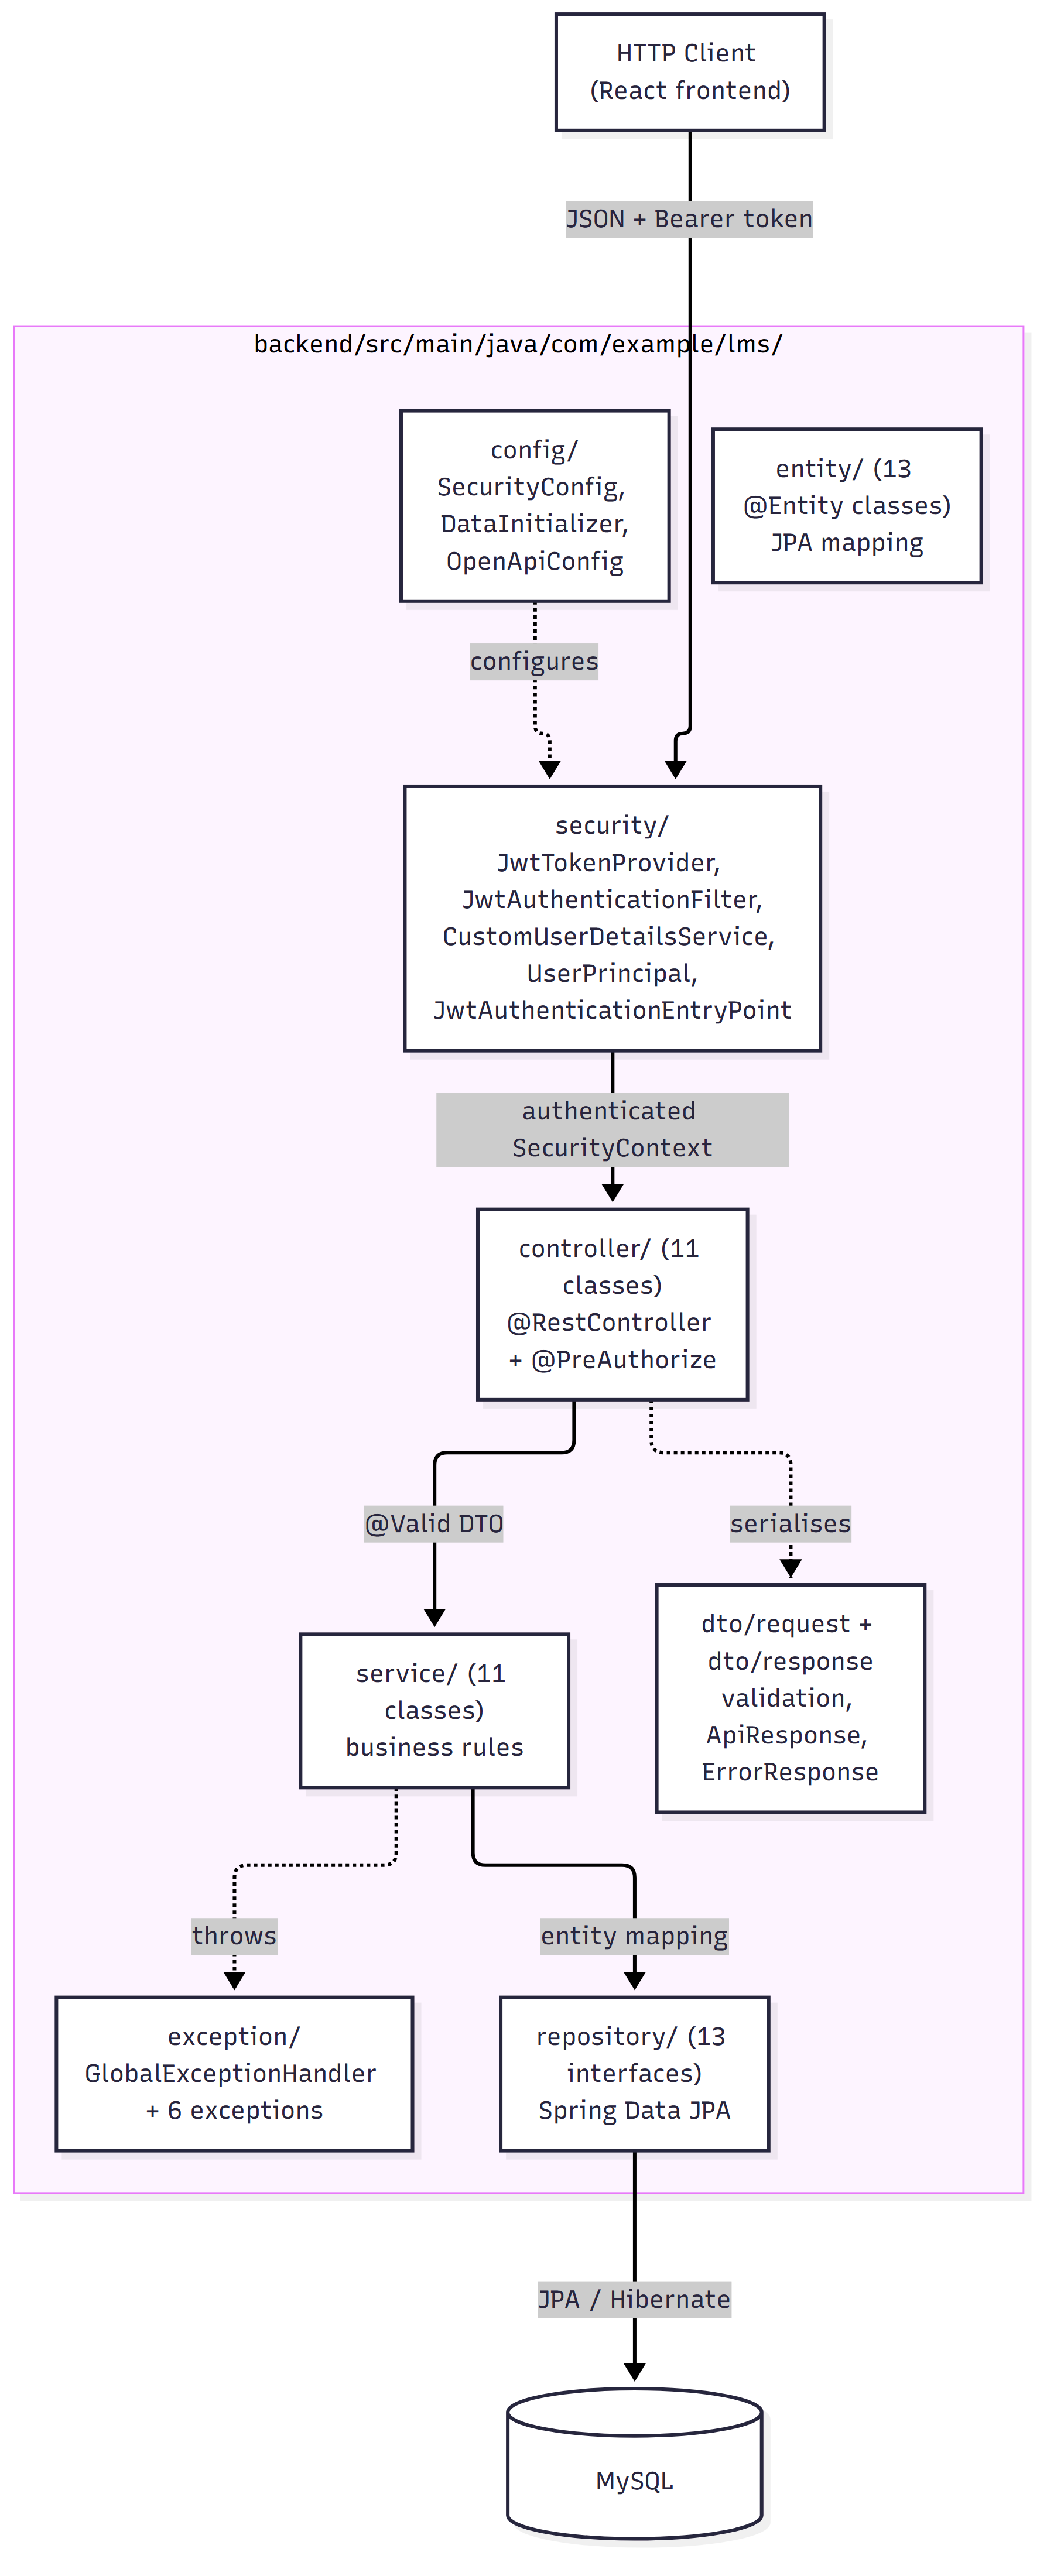
\includegraphics[width=0.92\textwidth]{diagrams/backend-layers.png}
\caption{Backend layering that every data flow traverses -- controller, service, repository}
\label{fig:data-layers}
\end{figure}

\subsection{What does not exist}
\status{IMPLEMENTED (absence verified)}

No event bus, message queue, cache layer, search index, object store, or background worker. No optimistic offline sync: the backend database is the single source of truth.

\section{UI/UX}
\label{sec:ui-ux}

\subsection{Page inventory}
\status{IMPLEMENTED}

Public: \code{/} (\pathref{frontend/src/pages/HomePage.jsx}), \code{/login}, \code{/register}, \code{/courses} (\pathref{frontend/src/pages/CourseCatalogPage.jsx}), \code{/courses/:id} (\pathref{frontend/src/pages/CourseDetailPage.jsx}), \code{/practice} and \code{/courses/:courseId/practice}. Authenticated: \code{/courses/:courseId/learn} (\pathref{frontend/src/pages/LearningPage.jsx}), \code{/quizzes/:id} (\pathref{frontend/src/pages/QuizTakingPage.jsx}), role dashboards (\pathref{frontend/src/components/LearnerDashboard.jsx}, \pathref{frontend/src/components/InstructorDashboard.jsx}, \pathref{frontend/src/components/AdminDashboard.jsx}), \code{/profile}, plus \code{*} fallback (\pathref{frontend/src/pages/NotFoundPage.jsx}).

\subsection{State contract}
\status{IMPLEMENTED}

Per CONTRACT.md section 16 every major page provides loading, success, empty, error and retry states; the frontend must never silently render empty data on API failure. Shared chrome lives in \pathref{frontend/src/components/Navbar.jsx} and \pathref{frontend/src/components/Footer.jsx}; reusable primitives live in \pathref{frontend/src/components/ui/} and \pathref{frontend/src/components/common/}.

\subsection{Responsive and accessible behaviour}
\status{IMPLEMENTED (with gaps)}

Tailwind utilities plus Ant Design components adapt desktop/tablet/mobile; cards must not overflow and forms must remain usable per the contract. \status{RECOMMENDED:} a systematic accessibility pass (focus order, labels, contrast audit against WCAG 2.1) is not evidenced in the repository.

\section{Design System}
\label{sec:design-system}

\subsection{Tokens}
\status{IMPLEMENTED}

The Ant Design theme in \pathref{frontend/src/App.jsx} sets \code{colorPrimary: \#000000}, 4px radius and 40px control height with component overrides; Tailwind tokens live in \pathref{frontend/tailwind.config.js}. Brand accents observed in code: gradient \code{linear-gradient(90deg, \#fc4c02, \#ef2cc1, \#bdbbff)} (\pathref{frontend/src/components/ui/GradientRibbon.jsx}), mint \code{\#c8f6f9}, dark canvas \code{\#010120}. Product brand is Edvanta (\pathref{frontend/index.html}, \pathref{frontend/src/components/Footer.jsx}).

\subsection{Component library}
\status{IMPLEMENTED}

Ant Design 5.22.2 provides tables, modals, forms, tabs and message toasts; project primitives in \pathref{frontend/src/components/ui/} (including \code{GradientRibbon.jsx}) and \pathref{frontend/src/components/common/} wrap them. Icons come from \code{@ant-design/icons} 5.5.2.

\subsection{Usage rule}
\status{RECOMMENDED}

New screens should reuse the App-level theme and Tailwind tokens rather than hardcoding colours or spacing, keeping the black-first Edvanta identity consistent.

\section{Security}
\label{sec:security}

\subsection{Implemented controls}
\status{IMPLEMENTED}

BCrypt password hashing, stateless JWT authentication with expiry (\pathref{backend/src/main/java/com/example/lms/config/SecurityConfig.java}), Bean Validation on DTOs, server-side role enforcement, consistent error envelopes that never leak stack traces or credentials, and JPA parameter binding (no string-concatenated SQL). Secrets are externalised through \pathref{.env.example} (\code{DB_URL}, \code{DB_USERNAME}, \code{DB_PASSWORD}, \code{JWT_SECRET}, \code{JWT_EXPIRATION}).

\subsection{Findings}
\status{IMPLEMENTED (gaps recorded, not invented)}

\begin{table}[H]
\centering
\caption{Security findings grounded in repository evidence}
\label{tab:sec-findings}
\begin{tabular}{@{}L{2.2cm}L{5.4cm}L{6.6cm}@{}}
\toprule
\textbf{ID} & \textbf{Finding} & \textbf{Evidence} \\
\midrule
S-01 & JWT in \code{localStorage}; no revocation or rotation & \pathref{frontend/src/context/AuthContext.jsx}; no refresh/token-blocklist code \\
S-02 & \code{DataInitializer} seeds demo users with hardcoded BCrypt passwords and no profile guard & \pathref{backend/src/main/java/com/example/lms/config/DataInitializer.java} \\
S-03 & Example \code{JWT_SECRET} committed in \pathref{.env.example}; must be rotated in production & File contents; no vault integration \\
S-04 & No rate limiting, lockout, password recovery, or email verification & Absence verified in controllers and config \\
S-05 & \code{ddl-auto: update} in configuration; schema history untracked & Backend application config \\
\bottomrule
\end{tabular}
\end{table}

\subsection{Production requirements}
\status{RECOMMENDED}

HTTPS, rotated secrets via a manager, CORS allow-list review, rate limiting on auth endpoints, security headers, audit logging, and removal or guarding of seed data before release. See OWASP Top Ten~\cite{owasp} and the JWT cheat sheet~\cite{owaspjwt}.

\section{Performance}
\label{sec:performance}

\subsection{Observed characteristics}
\status{INFERRED}

The application is a synchronous monolith with no cache, CDN, pagination contract, or query hints evidenced in the repository. Every list view is a direct JPA query; every interaction is a full HTTP round trip. No load-test results, budgets, or APM wiring exist in the repository (\status{UNKNOWN} for all numeric targets).

\subsection{Bottleneck risks}
\status{INFERRED}

Unbounded course/lesson/discussion listings, N+1-prone entity graphs, and server-side scoring loops are the most likely hotspots. The Vite production bundle (\code{npm run build} into \pathref{frontend/dist/}) is the only evidenced optimisation.

\subsection{Recommendations}
\status{RECOMMENDED}

Add pagination to list endpoints, index-verify slow queries against MySQL 8~\cite{mysql}, introduce response caching only after measurement, set performance budgets (e.g.\ catalogue p95), and instrument before scaling claims are made.

\section{Scalability}
\label{sec:scalability}

\subsection{Current posture}
\status{INFERRED}

The stateless JWT design allows horizontal scaling of the Spring Boot tier, but the single MySQL instance, file-less local state, and absence of caching, read replicas, or async processing bound vertical growth. No horizontal-scaling configuration (compose file, replica policy, migration runner) exists in the repository.

\begin{figure}[H]
\centering
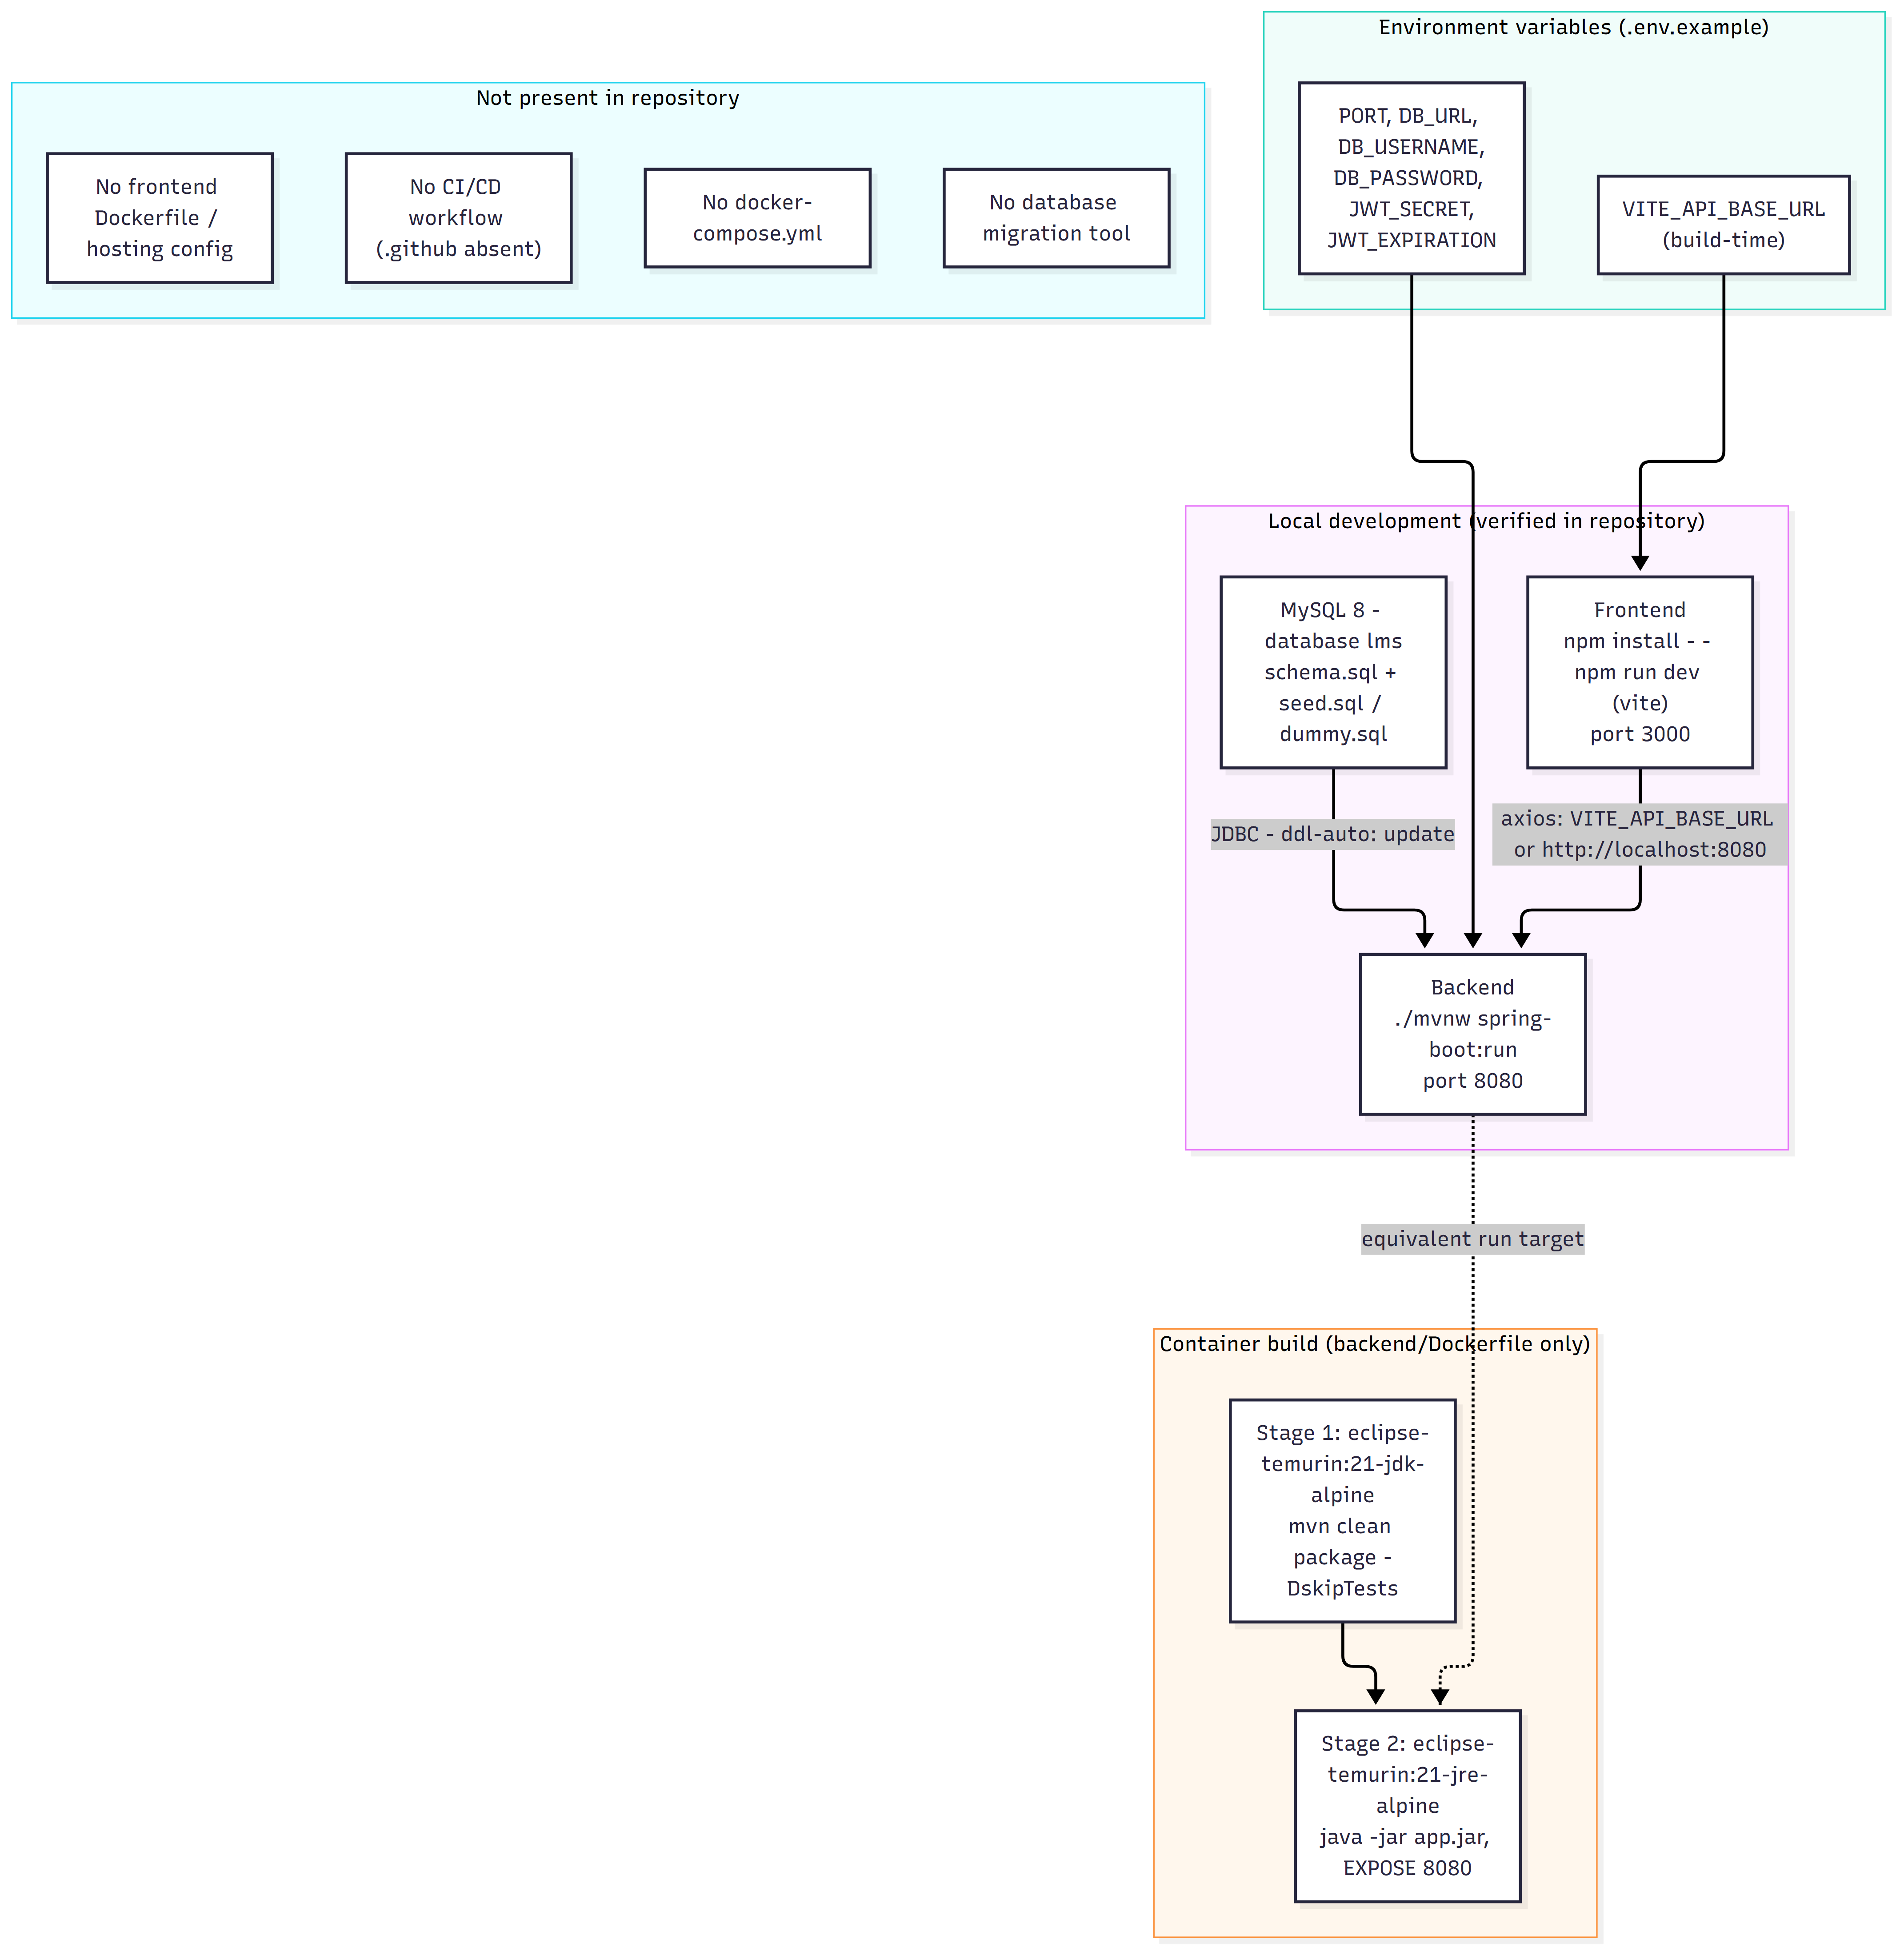
\includegraphics[width=0.9\textwidth]{diagrams/deployment.png}
\caption{Deployment view -- the only containerised component is the backend JAR}
\label{fig:deployment}
\end{figure}

\subsection{Scaling path}
\status{RECOMMENDED}

Containerise the frontend static bundle, add a compose or orchestrator topology, externalise sessions only if introduced, adopt versioned migrations before multi-instance deploys, then consider read replicas, caching, and CDN for static assets. Do not claim elastic scalability until the database and migration story are hardened.

\section{Testing}
\label{sec:testing}

\subsection{Backend tests}
\status{IMPLEMENTED}

22 test methods across 10 classes under \pathref{backend/src/test/}, including the end-to-end \pathref{backend/src/test/java/com/example/lms/integration/LmsIntegrationTest.java} (register, course, lessons, quiz, enroll, progress, certificate, discussion, feedback) with H2 as the test database. Run with \code{./mvnw test} from \pathref{backend/}.

\subsection{Frontend tests}
\status{IMPLEMENTED}

39 test methods across 8 files under \pathref{frontend/src/test/} using Vitest 2.1.8 with Testing Library and jsdom. Run with \code{npm test} (i.e.\ \code{vitest run}) from \pathref{frontend/}.

\subsection{Coverage contract}
\status{IMPLEMENTED (per CONTRACT.md sections 18--19)}

Backend must cover registration, login, invalid login, JWT validation, role authorization, course CRUD, enrollment including duplicates, progress, quiz submission and scoring, discussions, feedback, certificates, and invalid/unauthorized/forbidden/validation cases. Frontend must cover auth forms, route protection, catalogue, details, enrollment, lesson navigation, progress display, quiz interaction, results, discussions, feedback, certificates, dashboards, and loading/empty/error/responsive states. Five integration scenarios (register/login, enrollment, progress, assessment, certificate) must pass end to end.

\section{Deployment}
\label{sec:deployment}

\subsection{Verified development topology}
\status{IMPLEMENTED}

MySQL 8 on \code{localhost:3306} (schema from \pathref{database/schema.sql}) plus \code{./mvnw spring-boot:run} on :8080 plus Vite on :3000 with an \code{/api} proxy (\pathref{frontend/vite.config.js}). Backend base URL is configured once via \code{VITE_API_BASE_URL} (\pathref{.env.example}) and consumed through \pathref{frontend/src/api/client.js}.

\subsection{Containerisation}
\status{PARTIAL}

\pathref{backend/Dockerfile} is a multi-stage build (Maven on JDK 21 alpine, runtime on JRE 21 alpine, \code{EXPOSE 8080}). There is no frontend Dockerfile and no \pathref{docker-compose.yml}; production topology, TLS termination, backups, log shipping and health-check wiring are undefined.

\subsection{Production checklist}
\status{RECOMMENDED}

HTTPS, rotated secrets, managed MySQL with backups, versioned migrations, CORS allow-list, production JWT secret, structured logging, monitoring, and a defined rollback procedure. See also Sections~\ref{sec:cicd} and \ref{sec:configuration}.

\section{CI/CD}
\label{sec:cicd}

\subsection{Current state}
\status{IMPLEMENTED (absence verified)}

No \pathref{.github/} workflows, no pipeline configuration, and no automated gates exist in the repository. Builds and tests are manual: \code{./mvnw test} and \code{npm test} / \code{npm run build}.

\subsection{Recommended pipeline}
\status{RECOMMENDED (not implemented)}

On pull request: backend build plus tests, frontend install plus lint/typecheck plus tests plus production build, and a docs-link check. On merge to \code{main}: image build, migration dry-run, and staged deploy. Branch protections should enforce the CONTRACT.md review rules for shared files. No pipeline must be presented as existing.

\section{Integrations}
\label{sec:integrations}

\subsection{Embedded practice editor}
\status{IMPLEMENTED}

Course-attached coding practice embeds OneCompiler (\pathref{frontend/src/pages/practice/PracticePage.jsx}, \pathref{frontend/src/pages/practice/CoursePracticePage.jsx}, data in \pathref{frontend/src/data/}) via iframe with \code{postMessage} starter-code injection~\cite{onecompiler}. It is an isolated frontend dataset with no backend dependency by explicit design.

\subsection{External origins}
\status{IMPLEMENTED}

YouTube (lesson video references), Google Fonts, and Unsplash imagery are loaded as third-party origins outside the trust boundary and receive no user secrets.

\subsection{Not integrated}
\status{NOT APPLICABLE}

No payment gateway, email provider, SSO, analytics, or object storage is wired in v1.0 (explicitly excluded by CONTRACT.md section 5.2).

\section{Configuration}
\label{sec:configuration}

\subsection{Backend configuration}
\status{IMPLEMENTED}

Centralised Spring configuration (\code{application.yml} or equivalent) with sensitive values loaded from environment: \code{DB_URL}, \code{DB_USERNAME}, \code{DB_PASSWORD}, \code{JWT_SECRET}, \code{JWT_EXPIRATION}, \code{PORT} -- all documented in \pathref{.env.example}. Never commit real credentials; production must inject them through the environment or a secret manager.

\subsection{Frontend configuration}
\status{IMPLEMENTED}

The backend base URL is configured once as \code{VITE_API_BASE_URL} and referenced by every module in \pathref{frontend/src/api/} through the shared client. No component may hardcode \code{http://localhost:8080/api/...} (CONTRACT.md section 21).

\subsection{Database bootstrap}
\status{IMPLEMENTED}

\pathref{database/schema.sql} (13 tables), \pathref{database/seed.sql}, and \pathref{database/dummy.sql} define the hand-written schema; the runtime uses Hibernate \code{ddl-auto: update}. The drift risk between the two is recorded in Section~\ref{sec:technical-debt}.

\section{SEO}
\label{sec:seo}

\subsection{Current state}
\status{PARTIAL}

The SPA shell (\pathref{frontend/index.html}, Vite build into \pathref{frontend/dist/}) carries literal Edvanta metadata supporting ``LMS'', ``structured courses'', ``assessments'' and ``certificates''. Client-side rendering means crawlers see a thin shell; no sitemap, robots policy, canonical URLs, structured data, or prerendering is evidenced.

\subsection{Recommendations}
\status{RECOMMENDED}

Add unique titles/descriptions per public route (\code{/}, \code{/courses}, \code{/courses/:id}), semantic HTML, canonical links, a sitemap, and server-side rendering or prerendering for the catalogue if organic acquisition matters. Do not claim search visibility that has not been measured.

\section{AEO (Answer-Engine Optimisation)}
\label{sec:aeo}

\subsection{Current state}
\status{PARTIAL}

Course titles, descriptions and lesson text in MySQL are quotable answer sources, but no Q\&A schema, FAQ blocks, or extractable how-to summaries are provided for answer engines.

\subsection{Recommendations}
\status{RECOMMENDED}

Expose concise question/answer summaries per course (prerequisites, outcomes, duration), add FAQ structured data on public course pages, and keep factual claims (durations, levels, certificates) consistent between the UI and the API so assistants quote correct information.

\section{GEO (Generative-Engine Optimisation)}
\label{sec:geo}

\subsection{Current state}
\status{PARTIAL}

The same course/lesson corpus that serves learners is the only corpus generative engines could cite; no \code{llms.txt}, AI-use policy, or structured catalogue feed exists.

\subsection{Recommendations}
\status{RECOMMENDED}

Publish a machine-readable course catalogue summary, keep public descriptions factual and up to date, and define which content may be summarised or quoted by third-party assistants. No GEO capability is implemented until these artefacts exist.

\section{Known Issues}
\label{sec:known-issues}

\subsection{Recorded defects and inconsistencies}
\status{IMPLEMENTED (observations, not inventions)}

\begin{table}[H]
\centering
\caption{Known issues with repository evidence}
\label{tab:known-issues}
\begin{tabular}{@{}L{2.2cm}L{6.0cm}L{6.0cm}@{}}
\toprule
\textbf{ID} & \textbf{Issue} & \textbf{Evidence / impact} \\
\midrule
K-01 & \code{CertificateService} writes grade \code{DISTINCTION} while the column default is \code{PASS} & Cosmetic inconsistency in \code{certificates} rows \\
K-02 & Quiz percentage ignores unanswered questions (denominator only counts submitted questions) & Behaviour in quiz scoring service; inflates partial attempts \\
K-03 & README roadmap lists discussions/feedback as future work although both are implemented & \pathref{README.md} Phase~2 vs.\ discussion/feedback controllers \\
K-04 & Seed users with hardcoded passwords run on any empty database (no profile guard) & \pathref{backend/src/main/java/com/example/lms/config/DataInitializer.java} \\
K-05 & Hand-written \pathref{database/schema.sql} can drift from JPA entities under \code{ddl-auto: update} & No migration tooling; untested in CI \\
\bottomrule
\end{tabular}
\end{table}

\noindent Each item above is observable in the checked-in sources. Fixes belong on the roadmap (Section~\ref{sec:roadmap}) and must update the affected docs.

\section{Technical Debt}
\label{sec:technical-debt}

\subsection{Debt register}
\status{INFERRED (each item traces to repository evidence)}

\begin{table}[H]
\centering
\caption{Technical debt register}
\label{tab:tech-debt}
\begin{tabular}{@{}L{2.2cm}L{5.6cm}L{6.4cm}@{}}
\toprule
\textbf{ID} & \textbf{Debt} & \textbf{Consequence / remedy} \\
\midrule
TD-01 & No versioned migrations; \code{ddl-auto: update} & Schema history untracked; adopt Flyway/Liquibase \\
TD-02 & No CI/CD pipeline & Regressions undetected; add build/test gates \\
TD-03 & Seed data unguarded by profile & Demo accounts in prod risk; add profile guard \\
TD-04 & JWT without revocation/rotation & Cannot revoke sessions; add refresh + blocklist \\
TD-05 & Unbounded list endpoints | N+1 risk & Catalogue scale risk; add pagination, fetch plans \\
TD-06 & Frontend/backend contract only in prose & Drift risk; add OpenAPI diff check in CI \\
TD-07 & README roadmap drifted from code | missing LICENSE | no compose file & Onboarding friction; reconcile docs, add licence \\
\bottomrule
\end{tabular}
\end{table}

\section{Roadmap}
\label{sec:roadmap}

\subsection{Reconciled position}
\status{INFERRED}

\pathref{README.md} marks Phase~1 (core LMS) complete and Phases~2--4 unchecked, yet discussions and feedback are already implemented -- the README has drifted (K-03). The reconciled position: the core learning lifecycle is implemented and covered by an integration test; engagement, instructor-platform and advanced-platform items remain a mix of present and absent.

\subsection{Phased plan}
\status{RECOMMENDED (not committed scope)}

\textbf{Next (hardening):} fix K-01/K-02 scoring and grade consistency, guard seed data, adopt versioned migrations, add CI gates, rotate secrets, reconcile README. \textbf{Engagement:} notifications, learning analytics, improved learner dashboard. \textbf{Instructor platform:} authoring UX, lesson management, performance analytics. \textbf{Advanced:} certificate verification, search/filtering, recommendations, password recovery, monitoring, scalable deployment. CONTRACT.md section 5.2 exclusions (payments, live classes, mobile, AI tutoring, SSO, multi-tenancy) require formal agreement before work begins.

\begin{figure}[H]
\centering
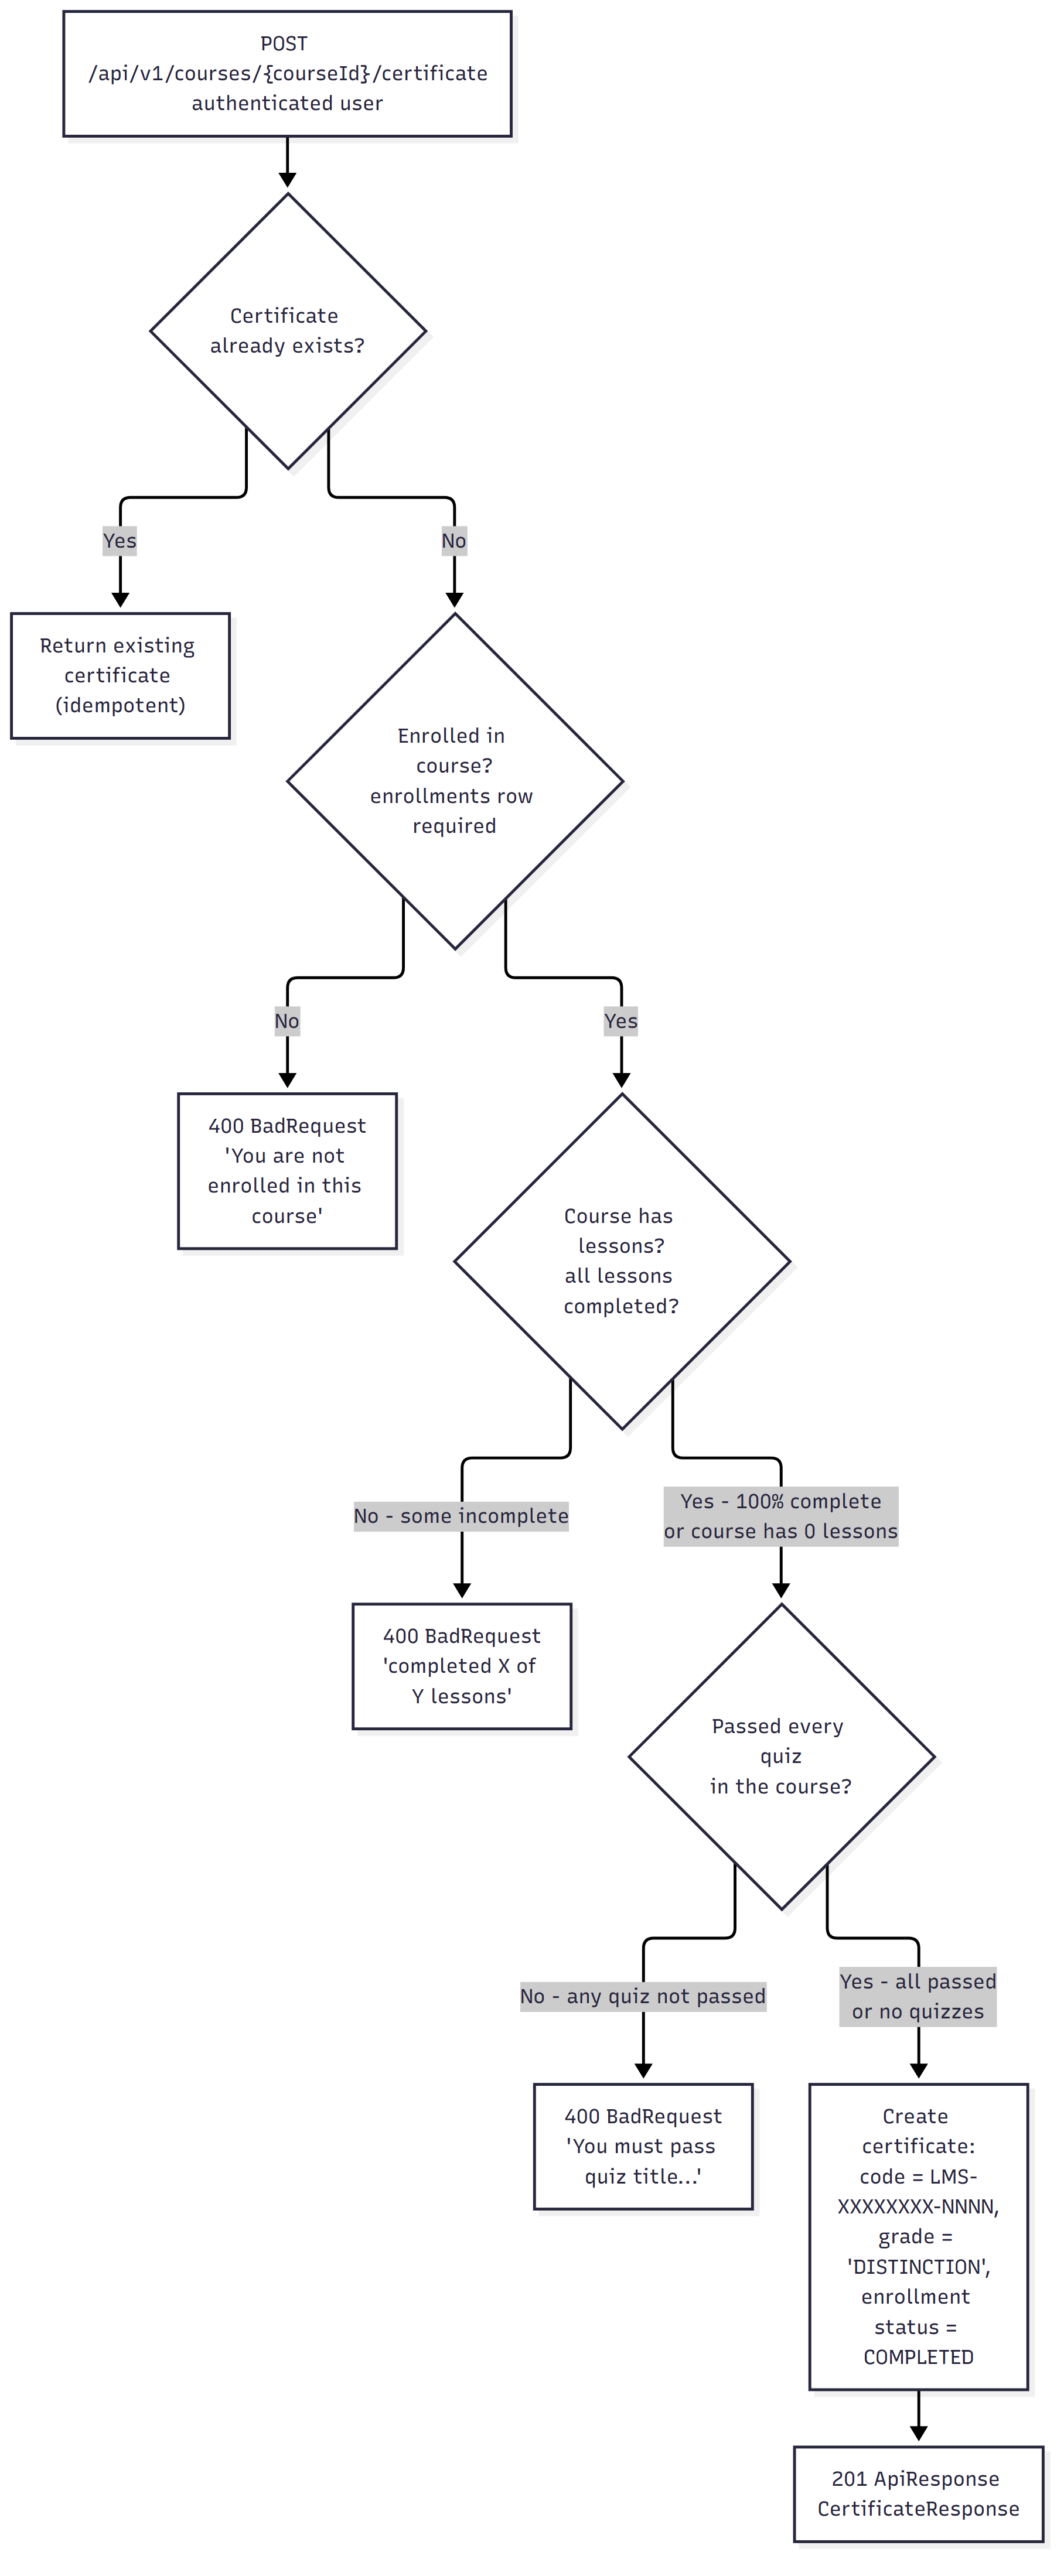
\includegraphics[width=0.9\textwidth]{diagrams/certificate-eligibility.png}
\caption{Certificate eligibility -- the gate all roadmap completion work must preserve}
\label{fig:cert-elig}
\end{figure}

\section{Development Guidelines}
\label{sec:development-guidelines}

\subsection{Layer discipline}
\status{IMPLEMENTED (per CONTRACT.md)}

Backend: controller (HTTP + validation) $\rightarrow$ service (business rules, transactions) $\rightarrow$ repository (persistence) $\rightarrow$ database; entities in \pathref{backend/src/main/java/com/example/lms/entity/}, contracts in \pathref{backend/src/main/java/com/example/lms/dto/}. Never place queries in controllers or business rules in DTOs. Frontend: pages in \pathref{frontend/src/pages/}, reusable UI in \pathref{frontend/src/components/}, backend communication only through \pathref{frontend/src/api/}, shared logic in \pathref{frontend/src/hooks/}, shared state in \pathref{frontend/src/context/}.

\subsection{Working rules}
\status{IMPLEMENTED}

Respect workstream ownership (\pathref{frontend/**} vs.\ \pathref{backend/**} + \pathref{database/**}); API and schema changes require agreement before integration; keep commits focused (\code{feat(frontend): ...}, \code{fix(backend): ...}); run \code{./mvnw test} and \code{npm test} before every PR; never commit secrets.

\section{Contribution Guide}
\label{sec:contribution-guide}

\subsection{Workflow}
\status{IMPLEMENTED (per CONTRACT.md sections 22--25)}

Develop on workstream branches (\code{frontend/...}, \code{backend/...}), never directly on \code{main}. Every PR states summary, changes, files, tests run, expected behaviour and known issues. Shared files (\pathref{README.md}, \pathref{CONTRACT.md}, \pathref{.env.example}, API and schema contracts, auth rules, major dependencies) require cross-workstream review. AI-assisted contributors must read \pathref{CONTRACT.md} and \pathref{README.md} first, stay inside the assigned workstream, follow canonical naming, and report failures honestly.

\subsection{Definition of Done (abridged)}
\status{IMPLEMENTED}

Feature, auth, course, enrollment, learning, assessment, discussion/feedback, certificate, frontend, backend and integration checklists in CONTRACT.md section 32 must all pass -- including real-backend integration with no required mock data and verified end-to-end flows.

\section{Glossary}
\label{sec:glossary}

\begin{table}[H]
\centering
\caption{Project glossary -- terms as used in this repository}
\label{tab:glossary}
\begin{tabular}{@{}L{3.6cm}L{10.6cm}@{}}
\toprule
\textbf{Term} & \textbf{Meaning} \\
\midrule
Edvanta & Product UI brand (title in \pathref{frontend/index.html}, footer in \pathref{frontend/src/components/Footer.jsx}) \\
Learner / Instructor / Admin & The three \code{users.role} values enforced by Spring Security and route guards \\
Course / Lesson & A course (\pathref{database/schema.sql} \code{courses}) owns ordered lessons (\code{lessons}, \code{order_index}) \\
Enrollment & Link between a learner and a course (\code{enrollments}, unique per user+course) \\
Progress & Per-lesson completion state aggregated to course percentage \\
Quiz / Question / Attempt / Result & Assessment chain: quiz owns questions; a submission creates an attempt scored server-side into a result \\
Discussion / Feedback & Course-scoped threads/replies and learner ratings \\
Certificate & Completion credential issued after server-side eligibility verification \\
DTO & Data-transfer object in \pathref{backend/src/main/java/com/example/lms/dto/} defining the API contract \\
JWT & Stateless signed token (JJWT 0.12.6) authorising API calls \\
springdoc & OpenAPI/Swagger generator serving \code{/v3/api-docs} and Swagger UI \\
Vite & Frontend build/dev server (port 3000, proxies \code{/api}) \\
\bottomrule
\end{tabular}
\end{table}


% ------------------------------------------------------------
% Appendix - references (external standards and official docs)
% ------------------------------------------------------------
\appendix
\section{References}
\label{sec:references}

The following external standards, specifications and official documentation were consulted for the technologies actually used in this repository. No fictitious citations are included.

\begin{thebibliography}{99}

\bibitem{springboot}
Spring Documentation.
\emph{Spring Boot Reference Documentation} (3.3.x).
\url{https://docs.spring.io/spring-boot/reference/}

\bibitem{springsecurity}
Spring Security Documentation.
\emph{Spring Security Reference}.
\url{https://docs.spring.io/spring-security/reference/}

\bibitem{springdatajpa}
Spring Data JPA Documentation.
\url{https://docs.spring.io/spring-data/jpa/reference/}

\bibitem{jjwt}
JJWT (JSON Web Token for Java).
\emph{JJWT 0.12.x Documentation}.
\url{https://github.com/jwtk/jjwt}

\bibitem{rfc7519}
IETF RFC 7519.
\emph{JSON Web Token (JWT)}.
\url{https://datatracker.ietf.org/doc/html/rfc7519}

\bibitem{rfc7517}
IETF RFC 7517.
\emph{JSON Web Key (JWK)}.
\url{https://datatracker.ietf.org/doc/html/rfc7517}

\bibitem{springdoc}
springdoc-openapi.
\emph{OpenAPI 3 for Spring Boot} (2.6.0).
\url{https://springdoc.org/}

\bibitem{openapi}
OpenAPI Initiative.
\emph{OpenAPI Specification 3.1}.
\url{https://spec.openapis.org/oas/latest.html}

\bibitem{react}
React Documentation.
\emph{React 18 -- Getting Started}.
\url{https://react.dev/}

\bibitem{reactrouter}
React Router Documentation (v6).
\url{https://reactrouter.com/}

\bibitem{vite}
Vite Documentation.
\url{https://vite.dev/}

\bibitem{vitest}
Vitest Documentation.
\url{https://vitest.dev/}

\bibitem{antd}
Ant Design 5 Documentation.
\url{https://ant.design/docs/react/introduce}

\bibitem{tailwind}
Tailwind CSS Documentation (v3).
\url{https://tailwindcss.com/docs}

\bibitem{axios}
Axios Documentation.
\url{https://axios-http.com/}

\bibitem{mysql}
MySQL Reference Manual (8.0).
\url{https://dev.mysql.com/doc/refman/8.0/en/}

\bibitem{hibernate}
Hibernate ORM Documentation.
\url{https://docs.jboss.org/hibernate/orm/current/reference/en/html_single/}

\bibitem{bcrypt}
\emph{The Bcrypt Password Hashing Function}, RFC 7914.
\url{https://datatracker.ietf.org/doc/html/rfc7914}

\bibitem{owasp}
OWASP Foundation.
\emph{OWASP Top Ten}.
\url{https://owasp.org/www-project-top-ten/}

\bibitem{owaspjwt}
OWASP Foundation.
\emph{JSON Web Token Cheat Sheet for Java}.
\url{https://cheatsheetseries.owasp.org/cheatsheets/JSON_Web_Token_for_Java_Cheat_Sheet.html}

\bibitem{webaim}
WebAIM.
\emph{Web Content Accessibility Guidelines (WCAG) 2.1 Overview}.
\url{https://www.w3.org/WAI/standards-guidelines/wcag/}

\bibitem{onecompiler}
OneCompiler.
\emph{Embed Code Editor}.
\url{https://onecompiler.com/embed}

\bibitem{pandoc}
Pandoc.
\emph{Pandoc User's Manual} (for optional DOCX conversion).
\url{https://pandoc.org/MANUAL.html}

\bibitem{mmdc}
Mermaid Live Editor / mermaid-cli.
\url{https://mermaid.js.org/}

\end{thebibliography}

\end{document}
